\documentclass[a4paper, 14pt]{extreport}
\usepackage[utf8x]{inputenc}
\usepackage[russian]{babel}
\usepackage{graphicx}
\usepackage{amsmath}
\usepackage{import}
\usepackage{xifthen}
\usepackage{pdfpages}
\usepackage{transparent}
\usepackage{xcolor}
\usepackage{calc}
\usepackage{setspace}
\usepackage{geometry}
\usepackage{titlesec}
\usepackage{listings}
\usepackage{color}
\usepackage{verbatim}
\usepackage[unicode, pdftex]{hyperref}
\geometry{a4paper, portrait, margin=15mm, bmargin=15mm, tmargin=20mm}
\graphicspath{ {./figure/} }

\hypersetup{
        colorlinks=true,
        linkcolor=black,
        filecolor=magenta,
        urlcolor=cyan,
        citecolor=black
}

\titleformat{\section}[block]{\normalfont\Large\bfseries\centering}{\thesection}{1ex}{}

\newcommand{\incfig}[1]{%
    \def\svgheight{\swgwidth}
    \import{./figure/}{#1.pdf_tex}
}

\newcommand{\anonchapter}[1]{\chapter*{#1}
\addcontentsline{toc}{chapter}{#1}
}

\definecolor{dkgreen}{rgb}{0,0.6,0}
\definecolor{gray}{rgb}{0.5,0.5,0.5}
\definecolor{mauve}{rgb}{0.58,0,0.82}
\definecolor{gray}{rgb}{0.4,0.4,0.4}
\definecolor{darkblue}{rgb}{0.0,0.0,0.6}
\definecolor{lightblue}{rgb}{0.0,0.0,0.9}
\definecolor{cyan}{rgb}{0.0,0.6,0.6}
\definecolor{darkred}{rgb}{0.6,0.0,0.0}


\lstset{
  basicstyle=\ttfamily\footnotesize,
  columns=fullflexible,
  showstringspaces=false,
  numbers=left,                   % where to put the line-numbers
  numberstyle=\tiny\color{gray},  % the style that is used for the line-numbers
  stepnumber=1,
  numbersep=5pt,                  % how far the line-numbers are from the code
  backgroundcolor=\color{white},      % choose the background color. You must add \usepackage{color}
  showspaces=false,               % show spaces adding particular underscores
  showstringspaces=false,         % underline spaces within strings
  showtabs=false,                 % show tabs within strings adding particular underscores
  frame=none,                   % adds a frame around the code
  rulecolor=\color{black},        % if not set, the frame-color may be changed on line-breaks within not-black text (e.g. commens (green here))
  tabsize=2,                      % sets default tabsize to 2 spaces
  captionpos=b,                   % sets the caption-position to bottom
  breaklines=true,                % sets automatic line breaking
  breakatwhitespace=false,        % sets if automatic breaks should only happen at whitespace
  title=\lstname,                   % show the filename of files included with \lstinputlisting;
                                  % also try caption instead of title  
  commentstyle=\color{gray}\upshape
  upquote=false, % Исправляет кавычки
}


\lstdefinelanguage{XML}
{
  morestring=[s][\color{mauve}]{"}{"},
  morestring=[s][\color{black}]{>}{<},
  moredelim=[s]{<?}{?>},
  morecomment=[s][\color{dkgreen}]{<!--}{-->},
  stringstyle=\color{black},
  identifierstyle=\color{lightblue},
  keywordstyle=\color{red},
  morekeywords={xmlns,xsi,noNamespaceSchemaLocation,type,id,x,y,source,target,tool,transRef,roleRef,objective,eventually}% list your attributes here
}

\definecolor{cmakegreen}{rgb}{0.0,0.5,0.0}
\definecolor{cmakemauve}{rgb}{0.58,0,0.82}

\lstdefinelanguage{CMake}{
    basicstyle=\ttfamily\small,
    keywords={project,cmake_minimum_required,add_executable,add_library,
              target_link_libraries,find_package,set,message,option,
              if,else,elseif,endif,foreach,endforeach,function,endfunction,add_compile_options,include_directories,
              ament_target_dependencies,install,ament_package},
    keywordstyle=\color{blue},
    comment=[l][\color{cmakegreen}]\#,
    stringstyle=\color{lightblue},
    morestring=[b]",
    morestring=[b]',
    sensitive=true,
    moredelim=[is][\textcolor{red}]{@}{@},
    moredelim=[s][\color{lightblue}]{\$\{}{\}},
    deletekeywords={VERSION,STATUS}, % Убираем лишние ключевые слова
    alsoletter={\$}, % Разрешаем $ в идентификаторах
}

\definecolor{keywordcolor}{RGB}{20,105,176} % Синий для ключевых слов
\definecolor{commentcolor}{RGB}{128,128,128} % Серый для комментариев
\definecolor{stringcolor}{RGB}{0,128,0} % Зелёный для строк
\definecolor{backgroundcolor}{RGB}{240,240,240} % Светло-серый фон

% Определение языка Dockerfile
\lstdefinelanguage{Dockerfile}{
  morekeywords={
    FROM, RUN, CMD, LABEL, MAINTAINER, EXPOSE, ENV, ADD, COPY,
    ENTRYPOINT, VOLUME, USER, WORKDIR, ARG, ONBUILD, STOPSIGNAL,
    HEALTHCHECK, SHELL
  },
  sensitive=true,
  morecomment=[l]{\#},
  morestring=[b]",
  morestring=[b]',
  keywordstyle=\color{neonpurple},
  commentstyle=\color{commentcolor},
  identifierstyle=\color{keywordcolor}
}

\definecolor{neonpurple}{RGB}{196, 21, 167}
\definecolor{deepred}{rgb}{0.6,0,0}
\definecolor{neongreen}{RGB}{34, 139, 34}
\definecolor{marsorange}{RGB}{183, 110, 46}
\definecolor{commentgreen}{RGB}{106, 153, 85}

\DeclareFixedFont{\ttb}{T1}{txtt}{bx}{n}{12} % for bold
\DeclareFixedFont{\ttm}{T1}{txtt}{m}{n}{12}  % for normal

% Определение стиля lstlisting для Python
\lstdefinestyle{customPython}{
  language=Python,
  morekeywords={self},              % Add keywords here
  keywordstyle=\color{neonpurple},
  comment=[l][\color{commentgreen}]\#,
  identifierstyle=\color{neongreen},
  emph={MyClass,__init__},          % Custom highlighting
  emphstyle=\color{deepred},    % Custom highlighting style
  stringstyle=\color{marsorange},
  frame=tb,                         % Any extra options here
  showstringspaces=false
}

\begin{document}
\begin{center}
        \textbf{Аннотация}
\end{center}
\par
\vspace{1cm}
\par В данной работе была рассмотрена разработка сетевого сервиса, для картографирования и локализации роботов. Сервис расширяет возможности бортового компьютера
 робота за счет взаимодействия с сетевым сервисом.
\par Основная задача работы: создать и продемонстрировать работу простейшего облачного сервиса, с возможностью удаленной настройки,
 наличием графического интерфейса пользователя и удобным получением информации с данного сервиса в формате данных ROS2 топика.
 В процессе разработки были рассмотрены:
\begin{itemize}
        \item Программные продукты, реализующие методы одновременного картографирования и локализации.
        \item Технологии дистрибуции сообщений, в частности FastDDS Discovery Server.
        \item Технологии контейнеризации, в частности Docker.
        \item Реализация графического интерфейса с использованием программной платформы Qt5.
        \item ROS2 экосистема и ее возможности для создания вычислительной сети.
\end{itemize}
\par\noindent Все алгоритмы в данной работе реализованны на языке C++, конфигурирование ROS2 файлов запуска пакетов на языке Python, создание микросервисов на языке
Dockerfile.
\tableofcontents
\anonchapter{Введение}
\textbf{Актуальность темы}
\vspace{5mm}
\par Сетевые технологии и сервисы широко используются для обеспечени многих критически важных инфраструктур в современном мире.
 Жизнь человека в 21 веке тесно связана с ними, у большинства людей при себе постоянно находится полная по Тьюрингу вычислительная 
 машина с выходом в глобальную сеть. Среди большого числа технологий и устройств, есть те, которые переросли единичное употребление
 и стали вектором развития для целой серии других открытий. Одна из подобных технологий, Internet of Things (IoT)\cite{iotBrief}\cite{iotPrep}, послужила основой
 для данной работы. 
\par Термин IoT, или Интернет вещей, обозначает некоторую инфраструктуру созданную между устройствами и сетевыми сервисами, часто принимающую вид
 некой вычислительной сети. Благодаря появлению недорогих компьютерных компонентов, 
 оптоволоконных технологий с высокой пропускной 
 способностью и других сетевых устройств, технология IoT стала набирать популярность. Появилось большое множество устройств, подключенных
 к Интернету и использующих возможности обработки данных сетевыми сервисами. Для компаний и людей, рынок умных товаров координально
 поменялся. Устройства, которыми люди пользуются повседневно, такие как зубные щетки, пылесосы, автомобили и автоматические установки,
 перестали нуждаться в громздких
 программах и вычислителях на борту. Для обеспечения собственной функциональности стало достаточно иметь необходимые датчики, доступ к глобальной сети
 и несколько мощных серверов для корректной работы устройств.
\par В связи с развитием технологии, многие робототехнические компании заинтересовались применением
 IoT в робототехнике. В результате, синергия классической робототехники и технологии IoT показала хорошие показатели. Дальнейшее изучение
 вопроса, создало новое направление в робототехнике - Облачная робототехника\cite{cloudRobotics}\cite{cloudPaper}.
\par Облачная робототехника - передний край исследований в области робототехники. В разработке Программного Обеспечения (ПО) по данной
 теме есть как устаявшиеся практики, так и пространство для новых. В данной работе, будет исследованы существующие решения
 и создано собственное Программное Обеспечение (ПО), поддерживающее технологию IoT.
\par В ходе предварительного анализа источников, был проведен сравнительный анализ роботов, использующих стандартную схему взаимодействия
 программных компонентов (на одном вычислителе) и роботов, использующих клиент/серверную или подобную архитектуру, для разделения задач
 между программными компонентами. В результате, роботы использующие разделение задач показывали значительный выйгрыш по ключевым показателям:
\begin{itemize}
        \item Загруженность CPU/GPU на бортовом компьютере робота. Необходимость объемных вычислений, как например, в алгоритмах одновременного
              картографирования и локализации, заставляет иметь мощный вычислитель, который повышает себестоимость робота и уменьшает время работы без подзарядки.
        \item Потребление заряда батареи. Роботы, использующие собственные вычислители потребляют больший ток на обеспечение их работы,
              к тому же, наличие батареи сильно увеличивает вес робота. В некоторых случаях больший вес, заставляет делать механику платформы в разы более сложной,
              что также требует дополнительных расходов как на инженерные работы, так и на конструкторские.
        \item Стоимость. За разработку сетевого сервиса и создание инфраструктуры из серверов платиться единоразовая плата, в то время как создание
              серии роботов, с мощными вычислителями на борту, заставляет платить за вычислитель каждый раз.
\end{itemize}
\par Выбор темы диссертации связан с актуальностью направления облачной робототехники, которая предлагает новые вызовые инженерам и программистам по всему миру.
 Также, тема связана с работами в области инфраструктурных задач в робототехнике, которые относятся к одному из направлений в области облачной робототехники.
\vspace{2mm}
\par\noindent\textbf{Цели и задачи}
\vspace{2mm}
\par Цель данной работы - разработка и реализация сетевого сервиса, который обеспечивал бы эффективное управление и запуск алгоритмов
 одновременного картографирования и локализации в контейнеризированной среде с использованием ROS2\cite{rosMain} и Docker\cite{dockerCommon}\cite{dockerPrep},
 а также создания графического пользовательского интерфейса для взаимодействия с данным сервисом на основе фреймворка Qt5\cite{qt5Book}\cite{qt5API}.
\par\noindent Среди задач данного исследования можно выделить следующие:
\begin{enumerate}
        \item Анализ существующих решений. Изучение современных методов использующихся при разрабоке сетевых сервисов, графических 
              интерфейсов пользователя, а также рассмотрение технологий для обеспечения сетевого взаимодействия и контейнеризации.
        \item Проектирование архитектуры системы. Выработка подхода для создания сетевого сервиса, графического интерфейса пользователя,
              создания сетевого взаимодействия, обеспечение платформенной независимости.
        \item Реализация сетевого взаимодействия.
        \item Реализация графического интерфейса пользователя.
        \item Тестирование сетевого сервиса. Проверка корректности работы, производительности и оценка эффективности взаимодействия.
        \item Анализ результатов. Проанализировать результаты тестирования, выявить преимущества и недостатки, обозначить вектор для
              дальнейших исследований и разработок.
\end{enumerate}
\vspace{2mm}
\par\noindent\textbf{Объект и предмет исследования}
\par Объектом исследования выступает информационно-техническая система - сетевой сервис, для управления алгоритмами одновременного
 картографирования и локализации в контейнеризированной среде.
\par Предметом исследований является методы и средства необходимые для разработки сетевого сервиса, обеспечивающего управление алгоритмами
 одновременного картографирования и локализации в контейнеризированной среде с использованием технологий ROS2 и Docker.
\vspace{2mm}
\par\noindent\textbf{Методы исследования}
\vspace{2mm}
\par Необходимо также указать основные методы исследования, которые были использованы в работе, среди них можно выделить теоретические и 
практические. Теоретические методы:
\begin{enumerate}
        \item Анализ и синтез. Данные методы используются для изучения существующих алгоритмов одновременного картографирования и
              локализации, сетевых протоколов, архитектурных решений и технологий, таких как ROS2, Docker, Qt5, Boost.Asio\cite{asioBook}\cite{asioPap} и т.п.
              Анализ позволяет разложить сложные системы на составляющие, а синтез - объединить полученные знания для разработки 
              собственной системы.
        \item Моделирование. Создание моделей, позволяет отразить структуру и возможные взаимодействия системы до ее реализации.
        \item Классификация и систематизация. Упорядочивание информации способствует более глубокому пониманию предметной области.
\end{enumerate}
\par\noindent В свою очередь эмпирические методы:
\begin{enumerate}
        \item Эксперемент. Проведение эксперемента поможет оценить успех выполненной работы.
        \item Наблюдение. Слежка за состоянием системы в различных сценарих работы является действенным способом для выявления
              возможных сбоев и анализа отклика системы.
        \item Измерение. Количественная оценка производительности системы, таких как время отклика, потребление ресурсов вычислительной
              машины, помогает сделать выводы о ценности данной системы для других.
        \item Сравнительный анализ - позволяет оценить преимущества и недостатки данного решения от подобных, выявить возможные пути 
              для улучшения и подтвердить или опровергнуть эффективность предложенного подхода.
\end{enumerate}
\vspace{2mm}
\par\noindent\textbf{Содержание и структура работы}
\vspace{2mm}
\par В данной работе реализован функционал сетевого сервиса для управления ROS2 узлами на удаленных серверах, применительно к
 задачам картографирования и локализации.
\par \textbf{Анализ существующих решений}. Современные архитектурные подходы к созданию сетевых сервисов, такие как микросервисная
 архитектура\cite{microServiceBook}\cite{microServiceBook1}, сервис-ориетированная архитектура (SOA)\cite{soaBook}\cite{soaBook1},
 бессервисная архитектура\cite{serverlessBook}\cite{serverlessBook1}\cite{serverlessArt1} и архитектура, управляемая событиями (EDA)\cite{edaBook}, предлагают 
 решения для обеспечения масштабируемости, гибкости о эффективности систем на их основе. Необходимо принять решение о выборе будущей архитектуры на основе 
 сильных и слабых сторон существующих архитектур. Также существует возможность использования комбинации различных архитектур для обеспечения требуемых 
 результатов. Наиболее распространенной архитектурой, на данный момент, является микросервисная архитектура, сочитающая в себе удобство масштабирования
 и гибкости, однако имеющая повышеные накладные расходы на запуск и поддержание микросервиса в случае большого количества одновременно запущенных сервисов.
 Важным моментом
 в создании решения является не только создание архитектуры сетевого сервиса, но и вопрос сетевого взаимодействия. Существует несколько
 основных протоколов\cite{protocolBook}\cite{protocolArt1} и технологий, использующих их для работы. Среди основных протоколов можно выделить протоколы: 
 \begin{itemize}
        \item HTTP - протокол, прикладного уровня, позволяющий работать со сложными программными сущностями (JSON, HTML, XML файлы и т.д.), обеспечивать шифрование и т.п.
        \item  WebSocket - проткол, позволяющий обеспечить постоянное двустороннее соединение между клиентом и сервисом.
\end{itemize}
 Немаловажной частью является рассмотрение существующих 
 решений в области построения графических пользовательских интерфейсов\cite{guiBrief}\cite{guiArt1}, где несомненным лидером является фреймворк Qt, позволяющий 
 строить эффективные, кросплатформенные интерфейсы на своей основе.
\par\textbf{Проектирование архитектуры системы}. Сетевой сервис должен обладать легким и понятным графическим пользовательским интерфейсом,
 эффективной работой с сетью и траффиком, а также быстро обрабатывать запросы пользователя. Для создания подобного решения необходимо использовать язык
 программирования 
 использования компилируемого языка программирования\cite{compLangArt}\cite{compLangBook}, который эффективно работает с памятью и
 процессором вычислительной машины за счет 
 низкой абстракции его команд, таким языком программирования является C++\cite{cppBook}\cite{cppArt1}. Многие крупные компании используют этот язык для написания 
 критически важных секций, т.к. данный язык имеет одну из самых близких к памяти и процессору их абстракций. Основной архитектурой 
 решения, будет выступать микросервисная архитектура с некоторыми дополнениями из клиент-серверной архитектуры, в качестве сервисов 
 будут выступать вычислительные машиные (далее сервера), которые будут запускать собственную серверную часть решения. В основе сетевого
 взаимодействия лежит асинхронные задачи связи созданные с помощью библиотеки Boost.Asio, позволяющей создавать TCP/UPD подключение между
 машинами в сети. Библиотека Boost в целом имеет нативную интеграцию с языком C++, множество решений из этой библиотеки были приняты 
 коммитетом по стандартизации языка C++, поддержка этих решений были включены в новые стандарты C++. Boost.Asio библиотека, которая 
 является дефакто стандартом для создания низкоуровневых абстракции сетевого взаимодействия является отличным решением для создания 
 инфраструктуры сетевого сервиса, однако, так как прямое соединение клиента и микросервисов напрямую возможно лишь в том случае, если
 микросервисы обладают так называемыми белыми ip адресами, то для тестирования решения будет использоваться локальный
 интерфейс связи, так называемый loopback, который позволяет тестировать решения не прибегая к созданию серверов с белыми ip адресами.
 Механизм связи при этом никак не изменится, потому что интерфейс loopback создает подобие локальной сети на компьютере и вполне может
 использоваться для создания условий в которых должен работать сетевой сервис. Проектирование графического интерфейса пользователя 
 позволяет создать удобный механизм для людей, уровня пользователей ПК, который даст им возможность пользоватся сетевым сервисом не 
 прибегая к изучению командной оболочки и документации к CLI для взаимодействия. Для создания графического интерфейса лучшим выбором 
 будет использования экосистемы Qt5, которая позволяет создавать удобные приложения на своей основе. Работу серверная сторона будет 
 вести над группой контейнеров, которые способны абстрагировать на заданом уровне процессы запущенные в них. Лучше всего для этого 
 подходит решение от компании Docker.inc, с одноименным названием. Контейнера смогут разделить задачи одновременного картографирования 
 и локализации по процессам в контейнерах, а связь между ними обеспечат механизмы взаимодействия ROS2 платформы. Таким образом будет
 создана гибкая, масштабируемая система из микросервисов, которые будут способны поддерживать выполнение алгоритмов одновременного 
 картографирования и локализации.   
% \par Анализ уже имеющихся в открытом доступе решений, показывает, что зачастую в подобных задачах используется клиент/серверная
%  архитектура, которая позволяет удаленным клиентам взаимодействовать с удаленными серверами. В данной работе, клиент/серверная архитектура
%  будет реализована для целей настройки облачной платформы. Для создания сетевого взаимодействия робота и платформы, так же будет
%  использоваться клиент/серверная архитектура, однако решение будет стандартное - использование FastDDS Discovery Server. Клиент/серверная
%  архитектура ключевой момент в создании всех современных веб-сервисов. Так же, из найденных данных становится ясным следующая, не менее
%  важная деталь - взаимодействие компонентов на облачном сервисе, или по-другому - топология. Многие использую для создании топологии
%  - программный каркас (фреймворк) Apache Storm, однако, для целей данной работы данный инструмент излишен, поэтому топология будет
%  построена с использованием технологий контейнеризации. В качестве инструмента контейнеризации будет использоваться Docker. Docker — это
%  программная платформа с открытым исходным кодом, предназначенная для управления приложениями в изолированных средах. Так же, многие
%  решения имею графический интерфейс пользователя, позволяющий клиентам, не имеющих специальных знаний в оболочках операционных
%  систем, использовать возможности без объемного инструктажа.
% \par Исходя из вышеизложенного, можно обобщить ключевые моменты, необходимые для создания Программного Обеспечения (ПО):
% \begin{enumerate}
%         \item Реализация клиент/серверной архитектуры, для задач удаленной настройки платформы.
%         \item Реализация клиент/серверной архитектуры, для задач сетевого взаимодействия робота и платформы. 
%         \item Реализация топологии.
%         \item Реализация графического интерфейса.
% \end{enumerate}
\vspace{2mm}
\par\noindent\textbf{Структура работы}
\vspace{2mm}
\par Работа состоит из введения, четырех глав и заключения.
\par Первая глава носит вводный характер и содержит основные понятия, методики работы, обозначения, механизмы взаимодействия и анализ 
существующих решений, которые позволяют создать необходимую инфраструктуру для сетевого сервиса и некоторые архитектурные моменты.
\par Вторая глава посвящена архитектуре сетевого сервиса для алгоритмов одновременного картографирования и локализации. В ней раскрыты
моменты анализа к требованиям системы, архитектура системы и проектирование графического интерфейса пользователя.
\par Третья глава посвящена деталям реализации сетевого сервиса для алгоритмов одновременного картографирования и локализации, показаны
ключевые моменты реализации, возможности библиотек, применительно к созданию и примеры использования.
\par Четвертая глава посвящена тестированию и оценке эффективности. Проведено сравнение с существующими решениями и приведены результаты
тестирования.
\vspace{2mm}
\par\noindent\textbf{Обзор литературы}
\vspace{2mm}
\par Был проведен поиск публикаций по теме. Далее будет перечислен список статей:
\begin{itemize}
        \item Supun Kamburugamuve, Leif Christiansen, Geoffrey Fox. - A Framework for Real Time Processing of Sensor Data in Cloud. - Indiana University:April 2015. - 12 p.
        \item Supun Kamburugamuve, Hegjing He, Geoffrey Fox. - Cloud-based Parallel \linebreak Implementation of SLAM for Mobile Robots. - Indiana University:December 2017. - 8 p.
        \item Chanda Monga, Minakshi Sharma, Sakshi Kalra. - Cloud Robotics. - Ferozepur City:March 2017. - 5 p.
        \item Rajesh Doriya, Paresh Payal, Vibhav Anand, Pavan Chakraborty. - A review on cloud robotics based frameworks to solve simultaneous localization and mapping (slam) problem. - National Institute of Technology:February 2015. - 6 p.
        \item Weinan Chen, Shilang Chen, Jiewu Leng, Jiankun Wang. - A Review of Cloud-Edge SLAM: Toward Asynchronous Collaboration and Implicit Representation Transmission. - IEEE Transactions on Intelligent Transportation Systems:November 2024. - 17 p. 
        \item Pengfei Zhang, Huaimin Wang, Bo Ding, Suning Shang. - Cloud-Based Framework for Scalable and Real-Time Multi-Robot Slam. - IEEE International Conference on Web Services (ICWS):July 2018. - 8 p.
        \item Supun Kamburugamuve, Hengjing He, Geoffrey Fox, David Crandall. - Cloud-based Parallel Implementation of SLAM for Mobile Robots. - ICC16:Proceedings of the International Conference on Internet of things and Cloud Computing. - 8 p.
        \item Taizhi Lv, Juan Zhang, Yong Chen. - A SLAM Algorithm Based on Edge-Cloud Collaborative Computing. - Hindawi Journal of Sensors:April 2022. - 17 p.
        \item Yanli Liu, Heng Zhang, Chao Huang. - A Novel RGB-D SLAM Algorithm Based on Cloud Robotics. - Microsoft Kinect Sensors: Innovative Solutions, Applications, and Validations:2019. - 28 p.
\end{itemize}
\par\noindent В статье "Cloud Robotics: A Survey" авторы предоставляют обзор технологий облачной робототехники. Они выделяют следующие основные преимущества облачной робототехники:
\begin{itemize}
        \item Масштабируемость: Облачная робототехника позволяет легко масштабировать роботизированные операции, добавляя или удаляя роботов по мере необходимости.
        \item Снижение затрат: Облачная робототехника может снизить затраты на роботизированные операции, поскольку предприятия могут использовать инфраструктуру и ресурсы облака вместо того, чтобы приобретать и поддерживать собственную инфраструктуру.
        \item Улучшенная безопасность: Облачная робототехника может улучшить безопасность роботизированных операций, поскольку данные и код могут быть централизованы и защищены в облаке.
\end{itemize}
\par\noindent Авторы также выделяют следующие основные недостатки облачной робототехники: 
\begin{itemize}
        \item Задержка: использование решений из области облачной робототехники могут привести к задержкам в роботизированных операциях, поскольку данные и команды должны передаваться через сеть.
        \item Безопасность: решения из области облачной робототехники могут представлять новые угрозы безопасности, поскольку зачастую данные предаются в незашифрованном виде, либо зашифрованными недостаточно.
        \item Сложность: решения из области облачной робототехники могут быть сложными для внедрения и использования, поскольку предприятия должны интегрировать в свои кодовые базы возможности взаимодействия систем робота с облачными сервисами.
\end{itemize}
\par Эти статьи описывают типичные подходы для решения задачи одновременного картографирования и локализации в облаке.
\chapter{Анализ предметной области}
\section{ROS2}
\par\noindent ​Robot Operating System 2 (ROS 2)\cite{rosMain}\cite{rosPrep} — это современная, модульная и масштабируемая платформа для разработки программного
 обеспечения в области робототехники и не только. Цифра 2 в названни означает версию данной платформы, данная версия пришла на смену
 традиционному ROS первой версии, устраняя его недостатки, в частности, недостаток настройки взаимодействия узлов в системе, однако
 ROS первой версии и ROS2 имеют много общего. Так, для конечного пользователя - программиста, ничего при роботе сильно не поменялось,
 только если некоторые инструменты сменили название и стали более эффективными, поэтому в дальнейшем, названия ROS и ROS2 будут 
 взаимозаменяемыми, в случае, если это не влияет на правильность повествования.
 ROS, был создан в 2007 году в Лаборатории Искусственного Интелекта Стэнфордского Университета и с тех пор стала одной из
 самых популярных платформ для созданиия Программного Обеспечения (ПО) в области робототехники. Данная платформа, активно
 поддерживается сторонниками открытого программного обеспечения, которые быстро исправляют различные ошибки обнаруженные 
 при работе с ROS и дополняют экосистему новыми инструментами. 
\par\noindent ROS, как и ROS2, предоставляет набор инструментов и библиотек для разработки Программного Обеспечения (ПО) для 
 целей робототехники. ROS2 использует микросервисную архитектуру, которая хорошо подходит для создания многокомпонентой,
 быстро изменяющейся системы. Одним из главных достоинств данной платформы для целей робототехники, является ее, относительно
 низкий, порог входа, от момента начала изучения до момента написания первого ROS2 узла проходит немного времени, т.к. ROS
 реализует многие абстракции самостоятельно, например, предоставляя реализацию сериализации данных с датчиков.
\par\noindent Основные возможности ROS 2, которые помогают в создании Программного обеспечения (ПО) для робототехники:​
\begin{itemize}
        \item Поддержки реального времени: так как, ядро ROS2 написано на C++, используя вычисления на этапе компиляции и 
         другие передовые практики при создании ПО обеспечивается низкие накладные расходы на использование.
        \item Масштабируемости: Использование сетевых возможностей, легко поддерживается работа в распределённых и многокомпонентных системах.
        \item Безопасности: Использование встроенных механизмов аутентификации и шифрования.
        \item Кросплатформеность: поддержка различных операционных систем и архитектур процессоров.
\end{itemize}.
\par В основе ROS2 находится Data Distribution Service (DDS)\cite{ddsMain}\cite{ddsBook} — стандартизированном протоколе обмена сообщениями, обеспечивающем
 надёжную и масштабируемую коммуникацию между компонентами системы. Этот протокол является приемником протокола первой версии ROS,
 который не только значительно расширил возможности к настройке взаимодействия компонент, но и так же, первый протокол, который 
 не был придуман разработчиками ROS, а просто был взят в качестве базы для ROS2.
\par\noindent Основные элементы архитектуры:
\begin{itemize}
        \item ROS2 демон (ROS2 daemon) - программа-демон, обеспечивающая работу всех механизмов.
        \item Узелы (Nodes): минимальные единицы компонентой системы, выполняющие определённые задачи.
        \item Топик (Topic): механизм обеспечивающий передачу сообщений между узлами.
        \item Сервис (Service): механизм синхронного взаимодействия между узлами, по аналогии с запросами и ответами в
         клиент/сервисной архитектуре.
        \item Действия (Actions): механизм поддержки длительных операций с возможностью отслеживания прогресса.
        \item Файлы запуска (Launches): механизм запуска группы узлов, позволяющий управлять временем и последовательностью
         запуска. Позволяет строить сложные последовательности запуска компонентой системы.
        \item Сервер параметров (Parameters Server): хранилище настроек каждого узла запущенного в системе. Позволяет изменять
         поведение узлов в процессе работы, а также отлаживать узлы при определенных настройках.
        \item Коммуникационный граф (Communication Graph) - абстракция взаимодействия узлов посредства​м топиков, сервисов и т.п.
\end{itemize}.
\par\noindent \textsl{\textbf{Замечание 1:} Демоном называется процесс, работающий в фоновом режиме без прямого взаимодействия с
 пользователем }
\par\noindent Эта архитектура обеспечивает гибкость и модульность, позволяя создавать сложные и надёжные робототехнические системы.
\subsection{Основы ROS2}
\par\noindent При первом использовании ROS2 становится заметной большая разница в работе, если раньше для обеспечения работы 
 механизмов требовался запуск ROS Master сервера - подобия сервера, через которого идет связь, то сейчас запуск компонентов
 можно осуществлять без него. Дело в том, что сейчас в основе ROS2 лежит Data Distribution Service (DDS), который использует
 автоматическое обнаружение других компонент, поэтому необходимость в сервере для обработки отпала, однако, в системе существует
 ROS2 daemon, который автоматически запускается вместе с компонентом, но вместо функции сервера для связи, он исполняет функции
 сервера для кэширования, позволяя ускорить процесс поиска других компонентов там, где это возможно.
\par\noindent \textsl{\textbf{Замечание 2:} Кэшированием называется хранение важные данных в высокоскоростной памяти, так 
кэшэ}
\begin{figure}[ht]
\begin{center}
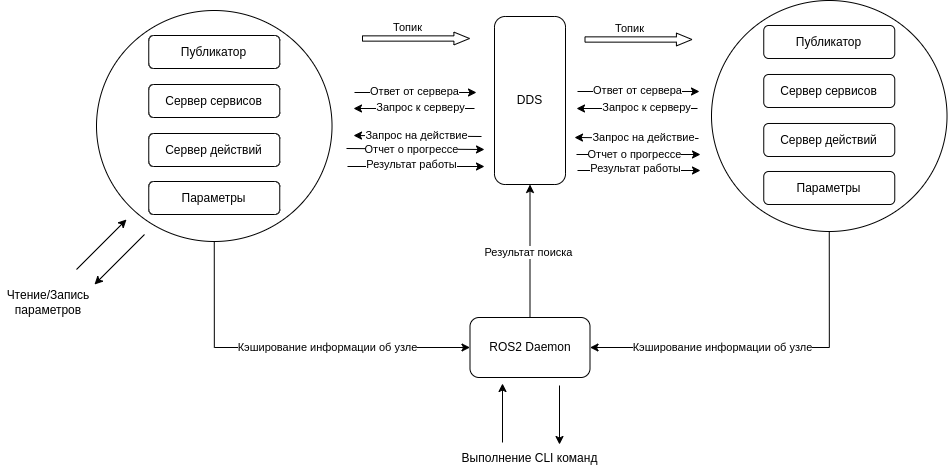
\includegraphics[scale = 0.5]{./figure/ros2_overview_schema}
\caption{Взаимодействие структурных частей}
\label{fig:manip_photo}
\end{center}
\end{figure}
\par\noindent После запуска хотя бы одной из компонент системы, при условии, что она публикует какие-то данные, используя топики, 
 можно увидеть список всех топиков в системе, для этого в новом окне оболочки системы следует запустить команду:
\begin{center}
        \par \textsl{ros2 topic list}
\end{center}
\par\noindent Каждый топик здесь, это отдельный от остальных, поток данных имеющий определенную структуру и тип. Используя ключ -v, 
 где v - от англ. verbosity, можно увидеть отображение имени топика на его тип, подробнее о типе можно узнать посмотрев соответствующую
 документацию. Для того, чтобы дублировать поток данных в оболочку существует команда:
\begin{center}
        \par \textsl{ros2 topic echo $\left[topic\_name\right]$}
\end{center}
\par\noindent где \(\left[topic\_name\right]\) - имя необходимого топика.
\par\noindent Существует несколько способов запуска ROS2 компонент, используя запуск единичного компонента и используя launch файлы,
 который запускают несколько компонент
\par\noindent Запуск единичного узла осуществляется с помощью команды:
\begin{center}
        \par \textsl{ros2 run $\left[pkg\_name\right]$ $\left[exe\_name\right]$}
\end{center}
\par\noindent Запуск launch файла осуществляется командой:
\begin{center}
        \par \textsl{ros2 launch $\left[pkg\_name\right]$ $\left[launch\_name\right]$}
\end{center}
\par\noindent где \(\left[pkg\_name\right]\) - имя необходимого пакета, \(\left[exe\_name\right]\) - имя исполняемого узла (ноды),
 \(\left[launch\_name\right]\) - имя launch файла. Пакетом , в данном случае, называется отдельный от других набор исходного кода,
 единой направленности.
\par\noindent Команды приведенные выше, являются основной частью Command Line Interface для ROS2 экосистемы, которые помогают 
 управлять работой и ускорять отладкой узлов. Command Line Interface содержит еще много команд, которые представляют интерес
 для разработчиков, подробнее о этой теме можно узнать по \href{https://docs.ros.org/en/humble/Tutorials/Beginner-CLI-Tools.html}{ссылке}
\subsection{Пакеты ROS2}
\par\noindent Пакетом в системе ROS2 называется некоторое множество кода единой направленности, которая удовлетворяет следующим
 критериям:
\begin{itemize}
        \item Адресуемость в окружении: кроме того, что пакет должен хранится на диске, чтобы с ним можно было взаимодействовать
              необходимо так же хранить его в определенной области, обычно папке, которая называется окружением. В данном окружении
              в дальнейшем, ROS будет искать компоненты для запуска и проводить сборку пакетов.
        \item Структура: файлы в пакете должны хранится согласно описаной в документации структуре, чтобы с ним можно было взаимодействовать.
        \item Наличие файла сборки: для сборки пакета и трансформации исходного кода в исполняемые файлы (компоненты) необходимо
              использовать файл, которые хранил бы в себе инструкции о том, каким образом компилировать и линковать файлы пакета
        \item Наличие файла метаинформации о пакете: для определения пакета ROS2 окружением, необходимо заполнить файл с метаинформацией.
              Эта информация помогает системе сборки корректно определять синтаксис файла сборки, зависимости от друих пакетов и т.п. 
\end{itemize}
\par\noindent Каждый из критериев следует расширить, для более полного понимания. Говоря о адресуемости, следует заметить, что 
окружение, обычно папка на компьютере, является местом хранения множества пакетов, которые, строго говоря, должны хранится в 
подпапке src окружения в отдельных папках, которые емко отражают направленность пакета. Например, название папки nav2, которая хранит
исходные коды пакета, явно указывает на то, что данный пакет реализует компоненты системы навигации. Переходя к следующему критерию -
структуре, необходимо добавить, что главное правило, которое необходимо соблюдать - наличие файла сборки, дальнейшие указания,
носят лишь рекомендательный характер. Файл сборки должен быть написан с использованием одного из языков систем сборки CMake\cite{cmakeBook}\cite{cmakeArt},
Python setuptools, Gargo и т.д. и ,соответсвенно, должны соблюдать и синтаксические правила этих языков. В данной работе, будет
использован язык системы сборки CMake, так как именно с помощью этого языка составляются файлы сборки пакетов написанных на языке
C++. Кроме того, ROS2 несколько расширяет функциональность стандартного CMake добавляя собственные функции, которые можно использовать
при сборке с использованием системы сборки colcon. Файл с метаинформацией о пакете, позволяет сделать пакет видимым для системы 
сборки colcon. В нем находится как информация о конфигурации файла сборки пакета, его зависимостях от других пакетов, экспортируемых
в оболочку переменных окружения, так и информация о разработчиках пакета, сайте проекта и т.п., но раскрытие данной информации 
происходит исключительно по желанию самих разработчиков. 
\begin{figure}[ht]
\begin{center}
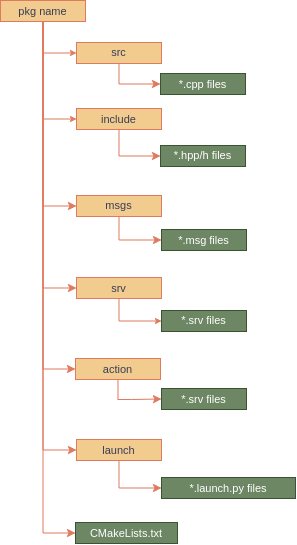
\includegraphics[scale = 0.5]{./figure/folder_schema}
\caption{Рекомендуемая структура пакета}
\label{fig:manip_photo}
\end{center}
\end{figure}
\par\noindent Немаловажной деталью темы пакетов является система сборки\cite{buildSystBook}\cite{buildSystArt}. В ROS2 системой сборки по-умолчанию является colcon. Colcon -
система сборки, используящая другие системы сборки, унифицируя их интерфейс для пользователя. Colcon поддерживает файлы сборки написанные
на языках CMake, Python setuptools и т.д. Colcon предоставляет Command Line Interface (CLI)\cite{cliBook}\cite{cliPrep} пользователям, с помощью которого можно
удобно и быстро собирать и тестировать пакеты. Местом, в котором система сборки и пакеты непосредственно соприкасаются и взаимодействуют,
называется окружением. Окружений может быть любое количество, однако, подобное зачастую не имеет смысла, так как, окружения существуют
для удобного размещения пакетов и уже собранных компонент пакетов. Окружение, как и пакет, имеет структуру, однако в отличии от пакета,
структура окружения задана в более строгой форме. Каждое окружение должно иметь подпапки src - подпапка в которой храняться пакеты,
install - подпапка в которой хранятся символьные ссылки на некоторые файлы из src, build - подпапка в которой храняться файлы необходимые
для сборки и log - подпапка в которой храняться файлы с информацией о запусках, сборках и т.п. Если подпапку src, пользователь
должен создавать сам, то остальные папки автоматически создаются системой сборки colcon во время первой сборки пакета в данном окружении.
\begin{figure}[ht]
\begin{center}
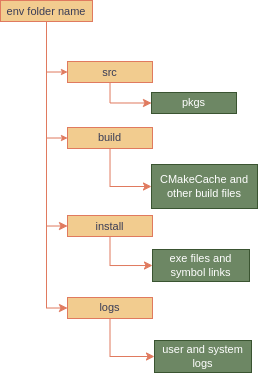
\includegraphics[scale = 0.5]{./figure/env_folder_schema}
\caption{Cтруктура окружения}
\label{fig:manip_photo}
\end{center}
\end{figure}
\par\noindent Сборка с помощью colcon осуществляется в корневой папке окружения с помощью команды:
\begin{center}
        \par \textsl{colcon build}
\end{center}
\par\noindent С помощью ключа -h (сокращение от help), можно вывести краткую справку по остальным ключам, среди наиболее полезных и 
 частоиспользуемых ключей находится ключи --symlink-install и --packages-select. Ключ --symlink-install позволяет создавать символьные
 ссылки на исходный код, который не нуждается в постоянной пересборке, например python исходный код, так как он является интропретируемым,
 а не компилируемым, следовательно, после его изменения не требуется его пересборка, это позволяет экономить время на сборку всего пакета,
 т.к. ссылка устанавливается один раз, а далее не требует обслуживания. Ключ --packages-select позволяет выбрать один или несколько
 пакетов, которые необходимо собрать, позволяя не собирать все пакеты, находящиеся в подпапке src окружения.
\par\noindent Рассмотрим процесс написания файла сборки на следующем примере:
\lstinputlisting[language=CMake,
                 firstline=1,
                 lastline=49,
                 frame=single,
                 xleftmargin=15pt,
                 caption={Файл сборки пакета eureka\_odometry},
                 label=DescriptiveLabel] {code/CMakeLists.txt} 
\par\noindent Данный файл сборки принадлежит пакету eureka\_odometry. Структура файла является стандартной для сборки небольших 
 C++ проектов, однако есть и некоторые новые функции, которые отличают этот файл сборки от подобных, предназначенных для сборки
 обычных проектов, без использования ROS2. Во-первых, разработчики создали инфраструктуру на CMake, которая позволяет находить
 другие пакеты, необходимые для сборки, используя стандартную функцию поиска find\_package, т.е. разрабочику больше не нужно
 писать собственные субпрограммы на языке CMake для поиска необходимых для сборки пакетов. Во-вторых, добавлены новые функции,
 которые упрощают процесс линковки библиотек из других пакетов, например, функция ament\_target\_dependencies(...), которая первым
 аргументом принимает цель, с которой нужно слинковать библиотеки, а следующими аргументами - имена пакетов из которых будут 
 выделены библиотеки.В-третьих, для обеспечения корректной работы системы сборки, необходимо наличие функции ament\_package(...),
 которая должна быть завершающей функцией в каждом файле сборки ROS2 пакета. Она позволяет, colcon проверять информацию о пакетах
 находящихся в файле с метаинформацией, создать скрипты оболочки позволяющие обнаруживать пакеты на компьютере с помощью ROS2 CLI
 комманд (CLI - Command Line Interface) и т.п.
\par\noindent \textsl{\textbf{Замечание 1:} Линковкой называют процесс связывания скомпилированных динамических библиотек в исполняемый файл. Является одним из этапов
 создания компилятором исполняемого файла из исходного кода в компилируемых языках программирования}
\par\noindent \textsl{\textbf{Замечание 2:} Динамической библиотекой называется скомпилированный особым способом исходный код, который связывается (линкуется) с пользовательской программой во время ее сборки}
\par\noindent Файл с метаинформацией о пакете, является не менее важной частью в процессе создания и регистрации пакета, поэтому ниже
 также будет расмотрен процесс создания на следующем примере:
\lstinputlisting[language=XML,
 frame=single,
 xleftmargin=15pt,
 caption={Файл метаинформации пакета eureka\_odometry},
 label=DescriptiveLabel] {code/package.xml} 
\par\noindent Рассмотрим ключевую информацию, необходимую для создания файла метаинформации. Во-первых, парный тэг <name>...</name>,
 в котором необходимо указывать имя пакета, аналогичное имя необходимо указывать в файле сборки внутри функции project(...).
 Во-вторых, парные тэги типа сборки - <buildtool\_depend>...</buildtool\_depend> и <build\_type>...</build\_type>, которые сообщают системе
 сборки об особенностях выбора подсистемы сборки, например, ament\_cmake, сообщает colcon о том, что для сборки будет
 использоваться система CMake и файла сборки написан с использованием языка CMake. В-третьих, парные тэги семейства depend, есть небольшое
 множестов тэгов этого семейства, среди которых <depend>...</depend>, <build\_depend>...</build\_depend>, <test\_depend>...</test\_depend>
 и <exec\_depend>...</exec\_depend>. Парный тэг <depend>...</depend> отдает управление зависимостью colcon, который должен определить
 к какому конкретному типу пренадлежит зависимость, другие тэги из семества определяют зависимость как зависимость сборки, тестирования,
 запуска соответственно. Тэги данного семейства позволяют управлять функциями подсистемы сборки, например, зависимость указанная
 как exec\_depend не может быть найдена через find\_package(...) CMake функцию в файле сборки и ,соответсвенно, не может быть слинкована
 с исполняемым файлом данного пакета, однако, должна быть найдена для успешной сборки пакета, так как может быть необходима для создания
 и запуска launch файлов (файлов запуска). 
\subsection{Использование ROS2}
\par Создание пакета и использование ROS2 CLI, является важной частью работы с ROS2 инфраструктурой, однако, полезную нагрузку создается
 именно наличие вычислительной сети из узлов и топиков. В ROS2 существует два способа запуска исполняемых файлов (узлов) - нативно с 
 помощью ROS2 CLI, или через launch файлы. Запуск узлов с помощью ROS2 CLI был рассмотрен выше, поэтому подробно остановимся на 
 запуске узлов с помощью launch файлов.
\par\noindent launch файл представляет собой инструкции по запуску узлов, в котором, кроме того может быть задана очередность запуска
, запуск вспомогательных утилит и много другое. launch файл может быть написан нескольких языках программирования, например на python
или xml. Рекомендуемым ROS2 сообществом языком для создания launch файлов является Python\cite{pythonBook}\cite{pythonBook1}, за его гибкость и хорошую интеграцию.
Ниже будет представлен листинг простого launch - а на языке Python с разбором основных моментов:
\lstinputlisting[style=customPython,
 frame=single,
 xleftmargin=15pt,
 caption={launch файл пакета eureka\_localization},
 label=DescriptiveLabel] {code/general.launch.py}
\par\noindent Первым блоком идет определение импортируемых функции, ROS2 сообщество основательно поработало над созданием функции
почти под все сценарии использования. Следующий блок обьявляет лист с аргументами, которые могут быть переданны launch - у пользователем
который запускает данный launch или launch - ем запускающим данный. Далее идет определение главной функции - generate\_launch\_description()
, в которой и происходит запуск всех необходимых узлов. С помощью функции LaunchConfiguration(...) переданные launch - у аргументы
могут быть захвачены и преобразованые в переменные с некоторым типом (так как Python не строго типизированный, то до конца не ясно
в какой), обычно в тип строки, и использоваться, например, для конфигурирования работы launch файла. Следующий блок захватывает 
программные пути к библиотекам с помощью функций библиотеки os, в качестве аргумента предается путь до папки с содержимым необходимого
пакета, в котором содержится исполняемые файлы (узлы) и вспомогательная информация. Данные папки содержаться в окружении в качестве
подпапки папки install. Для понимания дальнейших инструкции следует упомянуть о том, что launch файлы могут быть включены в другие 
launch файлы, т.е. при запуске может существовать верхнеуровневый launch, который будет запускать другие launch - и. Включение других
launch файлов осуществляется с помощью команды IncludeLaunchDescription, в которую, в качестве аргументов, передается путь до другого
launch файла и аргументы, которые должны быть переданы этому launch файлу, как если бы его запускали из командной строки. После инструкций
добавляющих launch файлы к запуску, идет инструкция запуска узла rviz2. Запуск узла осуществляется с помощью команды Node(...), в качестве
аргументов передается имя пакета, имя исполняемого файла (то имя, которое было задано в файле сборки), аргументы, как если бы запуск
происходил из командной строки, параметры, в форме \{имя параметра:значение параметра\} или в форме пути до .yaml файла с параметрами,
переопределения топиков - ROS2 дает возможность переименовывать топики для конкретного узла, это сделано потому что, узлы ожидают
определенный топик, а топики различаются, в основном, по имени. Далее идет непосредственно формирование списка из узлов, который 
будет передан ROS2 платформе. Список создается функцией LaunchDescription(...), которая в данном случае принимает аргументы launch - а,
однако, может принимать и список узлов, после чего следует передача сущности LaunchDescription непосредственно в экосистему ROS2 и 
запуск.
\subsection{FastDDS Server}FastDDS Discovery Server — это альтернативный механизм обнаружения узлов в ROS 2, заменяющий стандартный протокол
 Simple Discovery Protocol (SDP)\cite{sdpOverview}. Он решает ключевые проблемы масштабируемости и надежности в распределенных системах, таких
 как робототехнические платформы, IoT-сети и промышленные IoT-решения. В данной работе рассматриваются архитектура, функциональные возможности
 и практические примеры интеграции Discovery Server в ROS 2.
\par FastDDS Discovery Server — это альтернативный механизм обнаружения узлов в ROS 2, заменяющий стандартный протокол Simple
Discovery Protocol (SDP). Данный протокол помогает решить проблему масштабируемости в распределенной компонентной системе. В основе
лежит клент/серверная архитектура, в которой сервер выполняет роль клея для соединения узлов между собой, таким образом экономится
трафик, так как отсутсвет механизм multicast (вид поиска устройств в сети, при котором устройства посылает специального вида сообщение 
в надежде на ответ) и соединение идет напрямую через сервер.
\par\noindent Данный механизм имеет множество возможностей, в том числе и возможность создания резервных серверов для связи, создания
сохраняющих состояние во время сбоев и т.п., однако здесь будет расмотрены лишь основные возможности. Создание сервера происходит с 
помощью команды:
\begin{center}
        \par \textsl{fastdds discovery -l $\left[inteface\_ip\right]$ -p $\left[port\right]$}
\end{center}
\par\noindent после этого fastdds сервер будет слушать подключение к указанному ip и порту, чтобы воспользоваться связью через данный сервер
необходимо указать environment variable - переменную окружению ROS\_DISCOVERY\_SERVER с ip и портом сервера, например:
\begin{center}
        \par \textsl{export ROS\_DISCOVERY\_SERVER=127.0.0.1:11811}
\end{center}
\par\noindent после этого, все узлы публикующие сообщения в топики, будут связываться через fastdds сервер.
\section{Docker}
\par Docker — это программная платформа с открытым исходным кодом, предназначенная для автоматизации развертывания, масштабирования
 и управления приложениями в изолированных средах, называемых контейнерами. Контейнеры позволяют упаковать приложение вместе со 
 всеми его зависимостями, обеспечивая его стабильную работу в различных средах и упрощая процессы разработки и эксплуатации. 
 Docker был создан компанией docCloud.inc, как внутрений продукт компании, однако, после презентации проекта широкой публике,
 Docker быстро набрал популярность у программистов и системных инженеров, став мощным инструментом для инфраструктурных задач.
\par Основные компоненты Docker платформы:
\begin{itemize}
        \item Docker Engine: основной компонент, обеспечивающий создание, запуск и управление контейнерами.
        \item Docker Images: шаблоны, содержащие все необходимое для запуска приложения, включая код, библиотеки и зависимости.
        \item Docker Containers: изолированные среды, созданные на основе образов, в которых выполняются приложения.
        \item Docker Compose: инструмент для определения и управления многоконтейнерными приложениями с использованием YAML-файлов.
        \item Docker Hub: облачный реестр для хранения и распространения Docker-образов.​
\end{itemize}
\par Среди преимуществ использования данного решения в данной работе можно отметить:
\begin{itemize}
        \item Портативность: контейнеры Docker могут быть запущены на любой системе, поддерживающей Docker, что обеспечивает
              консистентность между различными средами разработки и эксплуатации.
        \item Изоляция: каждое приложение работает в своем контейнере, что предотвращает конфликты между зависимостями и
              обеспечивает безопасность.
        \item Масштабируемость: Docker облегчает горизонтальное масштабирование приложений путем запуска нескольких контейнеров одновременно.
        \item Быстрое развертывание: контейнеры запускаются значительно быстрее по сравнению с традиционными виртуальными машинами, что ускоряет
              процессы разработки и тестирования.
        \item Эффективное использование ресурсов: контейнеры используют ресурсы хост-системы более эффективно, чем виртуальные машины, что
              снижает затраты на инфраструктуру
\end{itemize}
\par\noindent Docker будет использоватся для построения топологии компонентов на облачной платформе. Контейнера будут абстрагировать
 программные компоненты, а точнее, ROS 2 ноды, в которых, уже существуют механизмы для управления потоками данных, таким образом,
 топология компонентов будет использовать комбинацию возможностей Docker для разделения программных компонент между собой и
 выстраивания инфраструктуры для сборки и запуска этих компонент, а выбор в сторону ROS2 программных компонент позволит управлять
 потоками данных между компонентами, давая легкую настройку этой связи.
\subsection{Основы Docker}
\par\noindent Под названием Docker в дальнейшем будет подразумеваться Docker Engine в связке с инфраструктурой (Docker Compose, 
 Docker Swarm и т.п.). Docker Engine - это ярдо платформы, представляющее собой сервер, который управляет контейнерами, образами и т.д.,
 которое к тому же, предоставляет REST API и Docker CLI, для взаимодействия с сервером. Если первый способ взаимодействия, через 
 REST API больше подходит приложениям, то вторым, через Docker CLI, обычно пользуются системные инженеры и программисты для удобной
 работы с Docker Engine сервером на компьютере. Использование возможностей данной платформы начинается с создания Dockerfile - ов и 
 понимания термина образ. Dockerfile - это набор инструкций для создания образа, а образ своеобразные слепок, по которому создаются
 контейнера. Рассмотрим создания простейшего Dockerfile и образа из него:
\lstinputlisting[language=Dockerfile,
 frame=single,
 xleftmargin=15pt,
 caption={Простой Dockerfile},
 label=DescriptiveLabel] {code/Dockerfile.simple}
\par\noindent Ключевое слово ARG - позволяет принимать аргументы переданные запускающей программой, чаще всего bash оболочкой, таким
 образом Dockerfile становятся конфигурируемыми. Далее FROM - ключевое слово, которое позволяет использовать любой образ имеющийся в 
 облачном регистре (при наличии интернет соединения) или на компьютере, в качестве базового для собирающегося образа. Ключевое слово
 RUN используется для выполенения комманд заданных пользователем. WORKDIR - просто устанавливает рабочую директорию и напрямую не 
 влияет на сборку. Выделим главные этапы сборки данного образа:
 \begin{enumerate}
        \item Выбор базового образа для текущего собираемого. Это позволяет упростить данный Dockerfile до простейших комманд над 
              заранее собранном образом.
        \item Создание аргументов. Повзоляет делать инструкции конфигурируемые не прибегая к редактированию файла.
        \item Загрузка дополнительных утилит. Опционально, однако, если образ на базе GNU/Linux\cite{unixBook}\cite{unixBook1}, позволяет экономить время и 
              использовать заранее скомпилированные программы.
        \item Создания инфраструктуры внутри будущих контейнеров данного образа. Опционально, однако также позволяет экономить 
              время, создавая общую для всех контейнеров инфраструктуру еще на этапе создания образа.
\end{enumerate}
\par\noindent Запуск сборки данного образа можно выполнить использовав POST запрос к DockerEngine демону, либо использовать вместо 
REST API CLI запрос, через командную оболочку. Воспользуемся вторым способом, так как он легче для понимания:
\begin{center}
        \par \textsl{docker build --tag $\left[new\_image\_name\right]$}
\end{center}
\par\noindent где \(\left[new\_image\_name\right]\) - название образа, по которому его можно будет идентифицировать. После запуска
 команды начнется процесс сборки, если на одном из этапов сборки произойдет ошибка, Docker закэширует данные о предыдущих этапах.
 После окончания процесса сборки, образ будет хранится в регистре Docker Engine демона, просмотреть какой идентификационный код 
 был присвоен демоном образу и другие данные о собранном образе можно с помощью команды:
\begin{center}
        \par \textsl{docker images}
\end{center}
\par\noindent Создать и запустить контейнер из собранного образа можно несколькими способами, один из них это указать в Dockerfile
 ключевое слово CMD, которое означает команду по-умолчанию, которая будет выполненна при создании и старте контейнера, созданного
 из данного образа, другим способом является создание и запуск контейнера "вручную", с помощью Docker CLI команды, третьим способом
 является создание docker-compose файла, который подобен по смыслу launch файлам из ROS2, с его помощью можно заранее определить 
 свойства целой группы контейнеров. Воспользуемся вторым по счету методом, и создадим контейнер с помощью Docker CLI, для этого 
 необходимо использовать комманду:
\begin{center}
        \par \textsl{docker run -it $\left[tag\right]$ $\left[command\right]$}
\end{center}
\par\noindent где \(\left[tag\right]\) - имя образа, которое мы передали с ключем --tag при его создании, а \(\left[command\right]\) - 
произвольная команда, которая будет выполененна оболочкой при старте контейнера. Просмотреть данные о запущенном контейнере можно
с помощью команды:
\begin{center}
        \par \textsl{docker ps}
\end{center}
\subsection{Преимущества Docker}
\par Docker остается одним из наиболее популярных решений для контейнеризации, особенно в контексте микросерверной архитектуры. Далее
буду рассмотрены альтернативы для контейнеризации и обоснова выбор Docker для данного исследования. Среди основных конкурентов Docker
можно выделить таких решения как Podman и LXC, оба этих решения являются средами для контейнеризации, кратко рассмотрим их преимущества
и недостатки.
\par\noindent Преимущества Podman:
\begin{enumerate}
        \item Повышенная безопастность. Так как система не имеет единого демона владеющего привелегиями root, то при взломе,
              злоумышленик не сможет управлять всеми контейнерами и потенциально, всей системой, также контейнера запускаются от имени
              пользователей, которые создаются Podman используя пространство имен пользователя GNU/Linux, что позволяет отследить 
              запуск до конкретного пользователя.
        \item Совместимость с Docker CLI. Возможность использовать Podman в качестве ядра и управлять им с помощью команд Docker CLI.
\end{enumerate}
\par\noindent Недостатки Podman:
\begin{enumerate}
        \item Менее зрелая экосистема. Из-за сравнительно небольшой популярности, отсутвует необходимая поддержка для экосистемы такого
              масштаба, следовательно многие функции существующие в Docker, не поддерживаются Podman.
\end{enumerate}
\par\noindent Преимущества LXC:
\begin{enumerate}
        \item Запуск контейнеров с полной операционной системой. Полноценная операционная система, является как сильной стороной, т.к.
              позволяет создать собственные сетевые интерфейсы, пользователей, пространства процессов и иметь собственную файловую
              систему, так и недостатком, т.к. наличие не несущих пользы возможностей накладывает ограничения на масштабируемость 
              подобных контейнеров.
        \item Гибкость. Тонкий процесс настройки потребляемых ресурсов.
\end{enumerate}
\par\noindent Недостатки LXC:
\begin{enumerate}
        \item Сложность в настройке. Гибкость и запуск контейнеров с полноценной операционной системой требуют соответсвующей квалификации
              у людей работающих с настройками данной технологии.
        \item Ограниченная поддержка сообщества. Сравнительно низкая популярность, вследствии чего, недостаток специалистов способных 
              развивать экосистему.
\end{enumerate}
В тоже время Docker, сочетает в себе гибкость, способность к масштабированию и сильную поддержку сообщества, которая делает данный инструмент
наиболее сбалансированным и поддерживаемым решением для данного проекта. Широкая экосистема, удобство использования делают Docker оптимальным
выбором для разработки и развертывания сетевых сервисов.
\section{Алгоритмы одновременного картографирования и локализации}
\par SLAM (Simultaneous Localization and Mapping)\cite{slamMain}\cite{slamArt0} — это метод, используемый автономными мобильными системами\cite{amrBook},
позволяющий одновременно
строить карту неизвестной среды и определять своё местоположение в ней. Эта технология стала ключевой в области робототехники, обеспечивая
навигацию без предварительно известной карты. Алгоритмы одновременного картографирования и локализации решают задачу одновременного 
построения карты окружающей среды и определения положения робота на этой карте путём обработки последовательности управляющих воздействий
и наблюдений, обновляя оценки положения и карты на каждом шаге времени. Основой большинства алгоритмов одновременного картографирования 
и локализации является использование фильтров на основе байесовского фильтра\cite{bayesBook}\cite{bayesArt}, позволяющий учитывать неопределённость и шум в данных.
\par Существует несколько основных видов алгоритмов одновременного картографирования и локализации по типу карты\cite{slamArt1} - метрические, 
топологические и семантические. Все алгоритмы построенные по метрическому типу используют для локализации байесовский фильтр,
в основе которого лежит байесовская рекурсия, которая обновляет апостериорное распределение состояния роботы и карты на каждом шаге:
\[
   P(x_k,m|Z_{0:k},U_{0:k}) = \eta P(z_k|x_k,m) \int P(x_k|x_{k-1},u_k) P(x_{k-1},m|Z_{0:k-1}, U_{0:k-1}) dx_{k-1}
\]
\par\noindent где:
\begin{itemize}
        \item \(x_k\) - состояние робота в момент времени k.
        \item \(m\) - карта окружающей среды.
        \item \(z_k\) - наблюдение в момент времени k.
        \item \(u_k\) - управляющее воздействие в момент времени k.
        \item \(Z_{0:k}\) и \(U_{0:k}\) - последовательность наблюдение и управляющих воздействия до момента k включительно.
        \item \(\eta\) - нормализующий множитель.
\end{itemize}
\par Это уравнение отражает двухэтапный процесс, на котором строятся байесовские фильтры:
\begin{enumerate}
        \item Прогноз - с помощью модели движения робота и управляющих воздейсвий предсказывается новое состояние \(P(x_k|x_{k-1},u_k)\)
        \item Коррекция - с помощью модели наблюдения и данных с сенсоров прогноз корректируется \(P(z_k|x_k,m)\)
\end{enumerate}
\par Все фильтры подобного типа основаные на марковских свойствах, т.к. текущее состояние зависит только от предыдущего и управляющих 
воздействий на шаге k. Алгоритмы данного типа создают карту привязаную к некой координатной системе, в которой объекты, имеющие
собственные размеры аналогичные реальным, привязаны к координатной системе.
\begin{figure}[ht]
\begin{center}
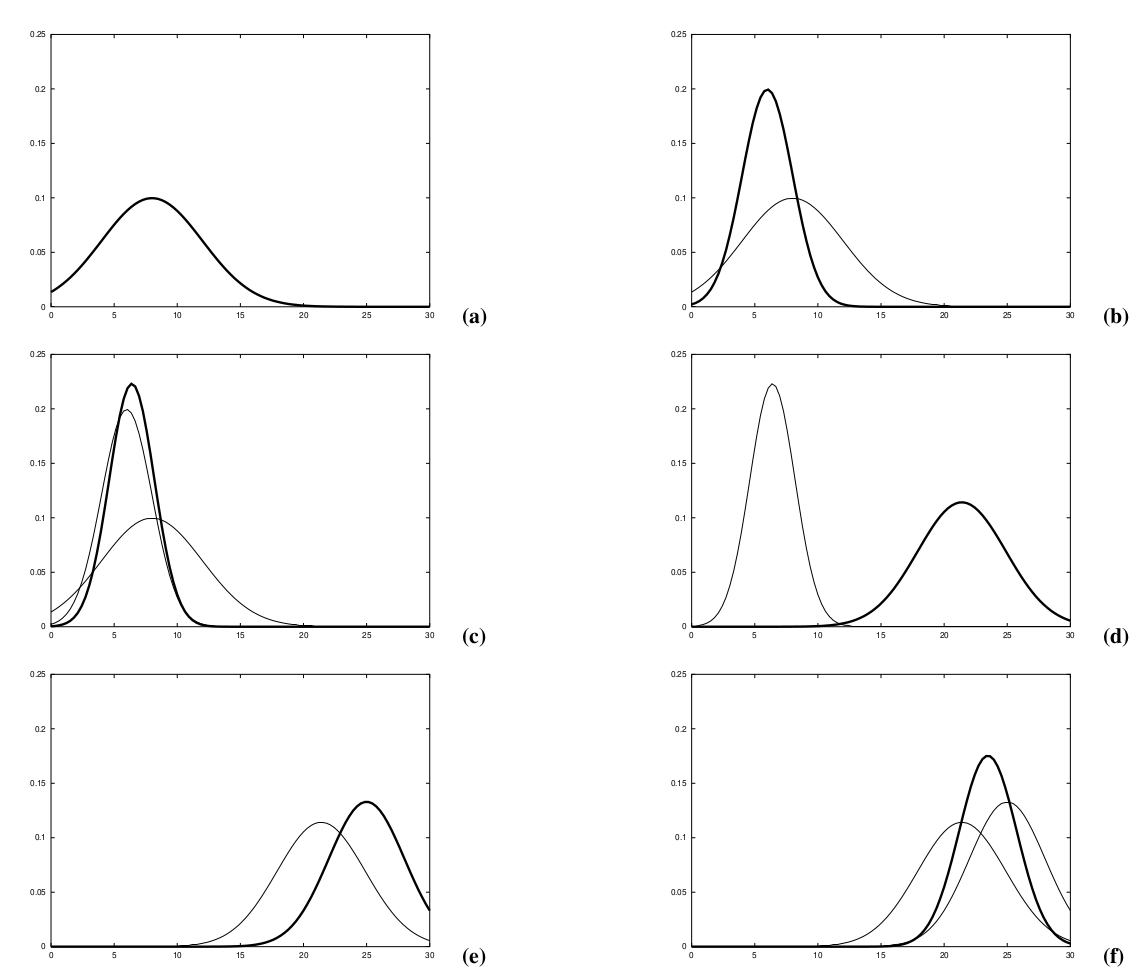
\includegraphics[scale = 0.3]{./figure/bayes_filter_process}
\caption{Процесс прогноза и коррекции в байесовском фильтре. График (a) представляет начальное распределение, (b) более темный график -
измерение со своим распределением, (c) распределение после интеграции измерения (коррекция), (d) распределение после некоторого управления (предсказание),
(e) более темный график - новое измерение со своим распределением, (f) распределение после интеграции измерения (коррекция)}
\label{fig:manip_photo}
\end{center}
\end{figure}

\par Более продвинутым вариантом метрических алгоритмов являются топологические алгоритмы\cite{slamArt2}, которые еще называют графовыми,
потому что окружающая среда в представлении алгоритма более походит на вершины, соединенные ребрами - возможными путями между вершинами.
Граф, как структура данных, используемая в топологических алгоритмах более всего подходит для создания карт больших или слабо
структурированных пространств. Основной задачей топологических алгоритмов является задача оптимизации\cite{slamArt3}, которая формулируется как задача
оценки траекторий и карты, основанных на зашумленных измерениях одометрии и наблюдаемых ориентиров. Цель заключается в нахождении 
конфигурации вершин, которая бы минимизировала суммарную ошибку между предсказанием и фактическим результатом. Математически задача 
формулируется следующим образом:
\[
   x = arg \hspace{1mm} min_{x} \sum_{(i,j) \in C} e_{ij}^T \Omega_{ij} e_{ij}
\]
\par\noindent где:
\begin{itemize}
        \item \(x\) - вектор состояния.
        \item \(e_{ij}\) - ошибка между измерением \(z_{ij}\) и предсказанным значением \(\hat{z}_{ij}(x_i, x_j)\).
        \item \(\Omega_{ij}\) - информационная матрица, обратная ковариации шума измерения, отражающая уверенность в измерении.
        \item \(C\) - множество всех пар связанных узлов \((i,j)\) в графе.
\end{itemize}
\par\noindent Эта формулировака основывается на предположении о гауссовском шуме и независимости измерений, что позволяет преобразовать задачу в 
минимизацию отрицательного логарифма правдоподобия. Таким образом, задача оптимизации направлена на нахождение вероятной конфигурации 
состояний, согласующейся с полученными измерениями. Для решения часто используют иттеративные методы, такие как метод Гаусса-Ньютона или 
алгоритм Левенберга-Марквардта, т.к. они их легко запрограммировать под вычислительные устройства. Эти методы требуют линеаризации функции 
ошибок вокруг текущей оценки и последующего решения полученной линейной системы уравнений:
\[
   H \Delta x = -b
\]
\par\noindent где:
\begin{itemize}
        \item \(H\) - матрица вторых производных.
        \item \(\Delta x\) - приращение оценки состояния.
        \item \(b\) - градиент функции стоимости.
\end{itemize}
\par\noindent После вычисления \(\Delta x\) текущая оценка обновляется:
\[
   x \leftarrow x + \Delta x
\]
\par\noindent Этот процесс будет повторяться до сходимости, т.е. до тех пор, пока изменения в оценке не станут пренебрежимо малыми.
Так же, топологические алгоритмы часто интегрируют в себя функциональность метрических алгоритмов, позволяя повысить
устойчивость системы.
\par Следующим витком развития алгоритмов одновременного картографирования и локализации являются семантические алгоритмы\cite{slamArt4},
способные не только создавать граф из особых объектов на карте и ,подобно метрических алгоритмам, знать расстояния между вершинами в этом 
графе, но и способны собирать информацию о контексте окружающей среды. Например, подобные решения, могут распознать кластер точек, который
является стулом и дать кластеру характеристику, что этот объект является стулом. В семантическом алгоритме, задача оптимизации усложняется,
т.к. кроме всего прочего, необходимо учитывать и семантику меток. Одним из подходов к такой задаче является формулировка задачи как 
оптимизации по фактор-графу\cite{slamPap1}, где узлы представляют состояния робота и объектов, а ребра - наблюдения и ограничения. Семантические алгоритмы строятся с использованием 
глубокого обучения позволяющий им осознавать контекст окружающей среды.
\[
   \theta = arg \hspace{1mm} max_{\theta} \sum_{t=1}^{T} \sum_{k=1}^{K_i} \log \left( \sum_{j=1}^{M} \omega_{t,k,j} p(z_{t,k}|x_t,m_j)\right) \\
   \text{, где} \hspace{2mm} \omega_{t,k,j} = p(a_{t,k} = j|\theta)
\]
\par\noindent Где:
\begin{itemize}
        \item \(\theta\) - параметры, включающие позы робота \(x_t\) и семантические ориентиры \(m_j\).
        \item \(z_{t,k}\) - наблюдение \(k\) в момент времени \(t\).
        \item \(\omega_{t,k,j}\) - вероятность того, что наблюдение \(z_{t,k}\) соответсвует семантическому ориентиру \(m_j\).
        \item \(p(z_{t,k}|x_t,m_j)\) - вероятность получения наблюдения \(z_{t,k}\) при позе робота \(x_t\) и семантическом ориентире \(m_j\). 
\end{itemize}
\par\noindent Эта формулировка учитывает неопределенность в ассоциации данных между наблюдениями и ориентирами, а также интегрирует 
семантическую информацию в процесс оптимизации.
\par Интеграция решения из области Облачной робототехники, к сожалению, пока всего лишь тенденция. Большинство компаний используют
алгоритмы одновременного картографирования и локализации, запускаемые на той же вычислительной машине, что и остальные критически важные
подсистемы. Это решение действительно обосновано, потому как алгоритмы должны быстро обрабатывать большой объем пространственных данных
с датчиков, однако, с развитием лазерной техники и производством новых оптоволоконных кабелей, стала возможной передача больших объемов
данных на больших расстояниях за приемлимое время, порядка 10 мс, что равно одной сотой секунды. Задержки такого порядка позволяют
использовать удаленные сервера для использования в задачах одновременного картографирования и локализации, которые работают с
периодчиностью подряка одной десятой секунды. То, что раньше считалось невозможным ввиду высокой задержки, вследствии чего алгоритмы использовали искаженное 
представление мира, не отражающее положение робота в реальности, сейчас может стать главным вектором развития робототехники и индустрии
умных устройств. Важно считаться и с тем, что и алгоритмы и микросхемы становятся все более оптимизированным, вследствии чего, не исключен 
тот факт, что использование решения на одной вычислительно машине, в будущем, окажется более жизнеспособным. 
\par\noindent Однако, на данный момент, в традиционном использовании алгоритмов мы все же сильно ограничены производительностью бортового
 компьютера робота, в то время как на сервере, возможно создать инфраструктуру из серверов любой сложности, которые бы справлялись в разы
 быстрее с обработкой данных с сенсоров. 
\par\noindent Проведем сравнительный анализ существующих алгоритмов одновременного картографирования и локализации и выберем наболее 
 оптимальный, на основе которого и будет работать сетевой сервис.
\par\noindent Критерием выбра алгоритмов для данного сравнительного анализа послужили количество "звезд" в репозитории проекта. Реализация
алгоритмов и их последующая интеграция проводится с использованием платформы ROS2.
\subsection{OpenSlam's Gmapping + AMCL/GMCL}
\par Связка из двух алгоритмов была рассмотрена не случайно, дело в том, что использование одного из них, без другого в целях одновременного 
картографирования и локализации невозможна. Пакет OpenSlam's Gmapping представляет из себя набор библиотек и инструментов для создания 
алгоритма одновременного картографирования и локализации, однако разработчиками, в качестве демонстрации функциональности был создан 
урезанный вариант алгоритма.
\par\noindent slam\_gmapping - главный узел в пакете OpenSlam's Gmapping, который представляет из себя реализацию алгоритма,
 использующего данные с плоского лазерного лидара, для картографирования и локализации на строящейся карте. Картографирование - главная
 цель этого програмного пакета, локализация здесь не представлена в явном виде (в виде топика). Следовательно локализацию из данного
 программного пакета нельзя получить, возможно лишь модифицировать его исходный код с целью получения топика с локализацией на карте.
 Данный алгоритм основан на фильтре частиц. Проект хорошо поддерживается, у него большое сообщество и много документации.
\par\noindent amcl - главный узел в пакете nav2\_amcl, который предоставляет реализацию алгоритма Adaptive Monte Carlo Localization (AMCL)\cite{amclArt}\cite{amclArt1}
 , который представляет собой адаптивные метод локализации робота в известной 2D-среде (на карте). Данный алгоритм реализует вероятностный
 подход с использованием фильтра частиц для оценки положения робота, как и алгоритм узла slam\_gmapping. Хорошо известен всему ROS 
 сообществу и является одним из наиболее популярных алгоритмов локализации использующихся на простейших мобильных платформах.
\par\noindent gmcl - главный узел пакета GMCL\cite{gmclArt}, алгоритм которого является потомком AMCL и предоставляет собой более усовершенствованную
 версию классического алгоритма. GMCL алгоритм вводит новые режимы для фильтра частиц - optimal, intelligent и self-adaptive, которые
 повышают эффективность распределения частиц, что позволяет улучшить производительность при работе в реальном времени. Пакет реализующий 
 алгоритм, не так хорошо известен, поэтому документация к нему достаточно скромная.
\par\noindent Работа с данной связкой возможна лишь при наличии плоского лазерного лидара, или его аналога. Так как алгоритмы реализованы 
с использованием платформы ROS2, то данные от сенсора к алгоритмам должные поступать строго по топикам и строго в виде 
sensor\_msgs/msg/LaserScan структуры.
\par\noindent\textbf{Репозитории:}
\begin{itemize}
        \item \href{https://github.com/Project-MANAS/slam_gmapping}{OpenSlam Gmapping на GitHub}
        \item \href{https://github.com/ros-navigation/navigation2/tree/main/nav2_amcl}{AMCL на GitHub}
        \item \href{https://github.com/adler-1994/gmcl}{GMCL на GitHub}
\end{itemize}
\subsection{hector\_slam}
\par Данный алгоритм одновременного картографирования и локализации\cite{hectorPap}, основанный на фильтре частиц, использует для работы плоские
лазерные лидары. Главным фактором конкурентноспособности является способность быстро обрабатывать большое количество данных. 
Быстрое встраивание новых кадров данных, и грубый этап сопоставления методом Гаусса-Ньютона на выходе дают удовлетворительную карту
окружающего мира. Чтобы воспользоваться преимуществами данного алгоритма одновременного картографирования и локализации, необходимо 
использовать плоский лидар, способный отправлять большое количество снимков в секунду. Хорошо зарекомендовал себя в ROS сообществе,
из-за удобства и эффективности.
\par\noindent Основным источником данных для данного метода картографирования и локализации является плоский лидар, однако возможно
использовать инерциальный датчик, который улучшит точность локализации.
\par\noindent\textbf{Репозитории:}
\begin{itemize}
        \item \href{https://github.com/tu-darmstadt-ros-pkg/hector_slam}{Hector SLAM на GitHub}
\end{itemize}
\subsection{rtabmap\_ros}
\par Данный алгоритм одновременного картографирования и локализации основан на графе\cite{rtabmapArt}. Все предыдущие методы так или иначе используют принципы
цепи Маркова, в которых текущее состояние является результатом изменений только предыдущего состояния. Метод графовых алгоритм использует 
цепи маркова немного по другому, позволяя создавать вершины в графе привязаном к карте. Данные вершины позволяют оптимизировать карту 
привязаную к ним прямо во время работы алгоритма. Rtabmap - является графовым алгоритмом не в прямом понимании, он лишь объединяет различные
методы локализации и картографирования и строит граф, привязаный к карте, чтобы оптимизировать его. Алгоритм способен работать сразу с 
большим числом источников данных, таких как, RGB камеры, RGBD камеры, плоские лазерные лидары, объемные лазерные лидары, сонары, дально
меры, энкодеры, инерциальные датчики ускорения, гироскопы и т.п. , причем количество датчиков одного типа ограничено лишь возможностями
процессора.
\par\noindent\textbf{Репозитории:}
\begin{itemize}
        \item \href{https://github.com/introlab/rtabmap_ros}{Rtabmap ROS на GitHub}
\end{itemize}
\subsection{cartographer\_ros}
\par Данный алгоритм одновременного картографирования и локализации, как и предыдущий, основан на графах\cite{cartographerArt}. Работает с сенсорами, который
способны выдавать данные в виде облак точек. Поддерживает функциональность картографирования и локализации сразу у нескольких роботов 
одновременно, что хорошо интегрируется в задачи облачных вычислений алгоритмов одновременного картографирования и локализации.
\par\noindent\textbf{Репозитории:}
\begin{itemize}
        \item \href{https://github.com/ros2/cartographer_ros}{Cartographer ROS на GitHub}
\end{itemize}
\par\noindent Компоненте amcl для корректной работы, нужна другая компонента - map\_server, которая является вспомогательной утилитой
для конвертации png, pgm и других форматов в сообщение типа nav\_msgs::OccupancyGrid для ROS системы и дальнейшей публикацией данного
сообщения в системе на топике map. После запуска вспомогательной компоненты мы должны передать топик, в котором публикуются данные с
сенсора, в данном случае лидара. Тип таких сообщений sensor\_msgs::LaserScan. Семантику других параметров для компоненты можно изучить
в документации для данного пакета.
\section{Технологии и инструменты разработки сетевых сервисов}
Прежде чем переходить к инструментам для разработки необходимо упомянуть об общепринятой модели сетевого взаимодействия - Open System
Interconnection (OSI)\cite{osiArt}\cite{osiArt1}. Модель разеляет сетевое взаимодействие на 7 уровне, каждый из которых выполняет определенные функции и поддерживается
определенным протоколом. Перечень уровней модели OSI:
\begin{itemize}
        \item Уровень 1: Физический - отвечает за передачу потока битов по кабелям. Протоколы: Ethernet, USB, DSL.
        \item Уровень 2: Канальный - отвечает за надежную передачу данных между узлами. Протоколы: Ethernet, Point-to-Point Protocol (PPP)
              Wi-Fi.
        \item Уровень 3: Сетевой - отвечает за маршрутизацию данных между сетями. Протоколы: Internet Protocol (IP), Internet Control 
              Message Protocol (ICMP), Address Resolution Protocol (ARP).
        \item Уровень 4: Транспортный - обеспечивает надежную связь между узлами. Протоколы: Transmission Control Protocol (TCP),
              User Datagram Protocol (UDP).
        \item Уровень 5: Сеансовый - отвечает за установку, поддержание и завершение сеансов связи. Протоколы: Remote Procedure Call (RPC).
        \item Уровень 6: Представление - отвечает за преобразование данных между форматами. Протоколы: SSL/TSL, MIME.
        \item Уровень 7: Прикладной - отвечает за предоставление сетевых сервисов конечным пользователям. Протоколы: HTTP/HTTPS, FTP, DNS,
              DHCP.
\end{itemize}
\par Это модель работы любого сетевого узла, именно благодаря созданию данной модели удалось распределить и стандартизировать механизм 
сетевого взаимодействия. Увеличение номера уровня отражает более абстрактные структуры данных, если на первом уровне модели протоколы
работают лишь с потоком битов, то на последнем, приложения работают со сложной структурой, заданной в протоколе. Поддержка всех 7 уровней 
позволяет разработчикам не думать о нижележащих уровнях модели, работая лишь с протоколом текущего уровня.
\par Для разработки сетевых приложений применяются множество фреймворков и библиотек, однако, не все из них подходят для задач создания 
всех механик сетевого сервиса с чистого листа. Часть библиотек используют протоколы верхнего уровня модели OSI, которые позволяют
абстрагировать сложные структурных
данных и сериализовать их при перессылке до потока битов, однако, для создания сетевого сервиса подобные решения не подходят, т.к.
абстракции использующиеся при этом не способные охватить необходимую информацию. Поэтому при создании сетевого взаимодействия
сервиса с чистого листа необходим собственный
протокол связи, т.е. необходимо создать набор структур, которые будут понимать и клиенты и сервера. Создание протокола - непростая задача, т.к. необходимо 
отказаться от заранее отлаженых механизмов верхнего уровня и создать их используя механизмы нижнего уровня. Так же, следует принять во 
внимание тот факт, что реализация сервиса планируется на языке C++, что накладывает ограничение на использование других языков, т.к.
лишь небольшое количество из других языков программирования имеют возможность управлять инструкциями на языке C++.Ниже представлен
перечень библиотек и фреймворки способных удовлетворить требованиям данного решения:
\begin{itemize}
        \item Boost.Asio - библиотека с открытом исходным кодом для синхронного/асинхронного ввода-вывода, поддерживающая протоколы
              TCP/IP уровня. Используется для создания высокопроизводительных сетевых приложений. Среди преимуществ - поддержка многих
              протоколов, обработка ошибок, асинхронность.
        \item POrtable COmponents (POCO)\cite{pocoDoc} - набор библиотек с открытым исходным кодом, позволяющая создавать кросплатформенные приложения,
              так же поддерживает работу с протоколами TCP/IP уровня и другими. Среди ключевых возможностей - модульная архитектура,
              поддержка большого количества протоколов, интеграция с C++ стандартом.
        \item Adaptive Communication Environment (ACE)\cite{aceBook} - объектно-ориентированный фреймворк на C++, предоставляющий набора классов для
              быстрого создания высокопроизводительных приложений. Среди ключевых возможностей - реализация шаблонов проектирования,
              поддержка структурами многопоточности, кросплатформенность. 
\end{itemize}
\par Появление первых версий межпроцессорного взаимодействия (IPC)\cite{ipcBook} и сетевых коммуникация случилось после появления операционной
системы UNIX версии 4.2BSD в 1983 году. Туда были добавлены новые программные сущности назваемые сокетами. Сокеты (от англ. - разъем)
- програмнные интерфейсы для обеспечения обмена данными между процессами, процессы не обазтельно должны исполняться на одном компьютере,
возможна и связь между разными компьютерами. К сокетам так же был добавлен соответсвующий API на языке C, функции которого можно было
вызвать из программы. Это существующая база на основе которой работают все современные приложения и операционные системы. Дело в том,
что при создании сетевого сервиса, можно было бы использовать только сокеты для создания сетевого взаимодействия и перессылке данных
между устройствами в сети, однако, для создания сложной логики выполнения необходимы большие затраты времени. Текущие библиотеки, 
используют сокеты в своей основе, при этом достаточно абстрагируя их и предоставляя пользователям новые механизмы для их использования.
Например, библиотека Boost.Asio способна создавать асинхронные задачи связи, которые пермещают буффер данных в хранилище и отправлют 
в тот момент, когда для выполнения есть мощности CPU.
\par В установлении сетевой коммуникации и пересылке данных многие моменты понятны, однако возникает вопрос с собственным протоколом 
связи. Существует множество протоколов связи, например, HTTP/HTTPS - протокол для передачи гипертекста или FTP - протокол для передачи
файлов и т.п., однако пользоваться таким протоколом в данном решении - излишне. Необходимо опустится ниже в модели OSI до протоколов
транспортного уровня и создать простой протокол, для перессылки собственной структуры данных. Создание сетевого протокола и задача 
выполнения абстракций лежащих ниже по уровням в модели OSI ложится на библиотеки из списка выше. Рассмотрим их и проведем сравнительный
анализ, который поможет выявить решение, которое ляжет в основу сетвого взаимодействия сервиса. Boost.Asio, POCO и ACE - три известные
библиотеки для сетевого программирования написанных на языке C++ и нативно поддерживающих его. Каждая из них имеет уникальные решения, 
однако среди всех выделяется библиотека Boost.Asio, с использованием которой напрямую или косвенно, связаны подовляющее большенство 
сетевых приложений и сервисов, выделяет ее не только большое сообщество, но и гибкость, эффективность и соотвествие современным 
стандартам C++. Boost.Asio предоставляет модель асинхронного ввода-вывода, которая позволяет эффективно управлять сетевыми операциями 
и ресурсами вычислительной машины. Ключевым в асинхронном механизме является io\_service, котороый координирует все асинхронные операции 
и управляет ресурсами, такими как сокеты и потоки, что обеспечивает высокую масштабируемость, прин низких затратах на использование 
абстракций вводимых Boost.Asio. В отличии от Boost.Asio, набор библиотек POCO ориентирован на пользовательские приложения работающие с 
существующими протоколами верхнего уровня - HTTP/HTTPS, SSL и т.п., что делает ее использование в качестве основы для создания 
протокола затруднительной, однако, нельзя не учесть ее удобсто в быстром создании сетевых сервисов на базе высокоуровневых протоколов.
Кроме того, POCO имеет меньшее сообщество энтузиастов и ограниченную документацию, которая делает создания и поддержку сетевого сервиса
с чистого листа еще более сложной задачей. Переходя к рассмотрению достоинств и недостатков фреймворка ACE, нельзя не учесть широкий 
набор инструментов для разработки, включая поддержку шаблонов проектирования\cite{patternBook}\cite{patternArt1} и компонентов безопастных к 
многопоточности\cite{concurrBook}\cite{concurrArt1}. Однако 
широкий набор инструментов делает этот фреймворк сложным в освоении. Использование данного решения приведет к работе с большим объемом
кода, что может привести к непозволительному увеличению времени разработки и усложнит поддержку сетевого кода на основе данного решения.
Таким образом, при создании сетевого сервиса с чистого листа библиотека Boost.Asio является единственно верным решением, на базе которого
будет построен гибкий и производительный компонент системы предназначенный для сетевого взаимодействия.
\chapter{Проектирование архитектуры сетевого сервиса}
\par Эта глава будет полность посвящена архитектуре создаваемого сетевого сервиса для алгоритмов одновременного картографирования и 
локализации. В ней будут сформулированы основные требования к системе, рассмотрена диаграма классов из UML\cite{umlArt} для данного решения, выстроена
модель сетевого взаимодействия и показаны основные моменты проектирования графического интерфейса пользователя, которым будет обладать 
клиентская часть сервиса. Начнем с анализа требований к системе.
\section{Анализ требований к системе}
\par Исходя из особенностей архитектуры системы ниже представлен струтурный подходи к анализу требования, которым система должна следовать 
чтобы обеспечить надежность, масштабируемость и эффективность.
\par\noindent Функциональные требования:
\begin{itemize}
        \item Микросервисная архитектура - каждый сервис должен выполнять одну конкретную функцию и быть независимым от других.
              Масштабируемость и низкие накладные расходы на создание каждого сервиса являются приоритетом. Docker обеспечит изоляцию и 
              портируемость таких сервисов, позволяя легко управлять их жизненным циклом.
        \item Поддержка обмена сообщениями с помощью ROS2 - ROS2 предоставляет механизм топиков на основе Data Distribution Service, для
              обмена сообщения между узлами в микросервисах и между микросервисами и роботами, пользующимися сетевым сервисом. Это также 
              обеспечит высокую степень гибкости и масштабируемости, без особых накладных расходов.
        \item Асинхронная клиент-серверная связь через Boost.Asio - Boost.Asio предоставляет средства для реализации асинхронной сетевой 
              коммуникации между микросервисами и супер-клиентом, имеющим возможность настройки микросервисной архитектуры. Асинхронная 
              связь позволяет эффективно обрабатывать множество одновременных соединений, что позволит использовать целые кластеры 
              микросервисов.
        \item Взаимодействие с Docker через Web API\cite{dockerApi} - Сервер управляющий микросервисами должен имет возможность управлять контейнерами 
              через RESTful API Docker демона, обеспечивая автоматизацию процессов развертывания и мониторинга.
\end{itemize}
\par\noindent Нефункциональные требования:
\begin{itemize}
        \item Производительность - система должна обеспечивать низкую задержку и высокую пропускную способность, особенно при обмене 
              сообщениями между микросервисами и клиентом.
        \item Масштабируемость - ключевой фактор, архитектура должна поддерживать горизонтальное масштабирование, позволяя добавлять
              новые экземпляры сервисов без накладных расходов на программирование.
        \item Надежность и отказоустойчивость - система должна продолжать работу даже при отказе отдельных компонентов.
\end{itemize}
\par Таким образом, исходя из требований к системе можно перейти к этапу проектирования системы. Архитектуру системы состоит из двух 
основных частей, первая часть это супер-клиент с графическим интерфейсом пользователя, вторая часть - сервер взаимодействующий с 
микросервисами, которые в свою очередь взаимодействуют с роботом. Под супер-клиентом здесь подразумевается устройство, не являющееся 
роботом, в следствии чего не нуждающейся в большей части информации с микросервисов, служащее для настройки серверов по средством 
графического интерфейса пользователя. Сервер же, устройство, напрямую взаимодействующее с микросервисами и управляющее ими. 
Микросервисы - контейнера Docker, способные передовать информацию серверу через Docker Web Api и способные передавать информацию роботу
по средствам FastDDS Discovery Server - а запущенного на каждом из доступных серверов. Рассмотрим структуру компонентов и их 
взаимодействие на рисунке:
\newpage
\begin{figure}[ht]
\begin{center}
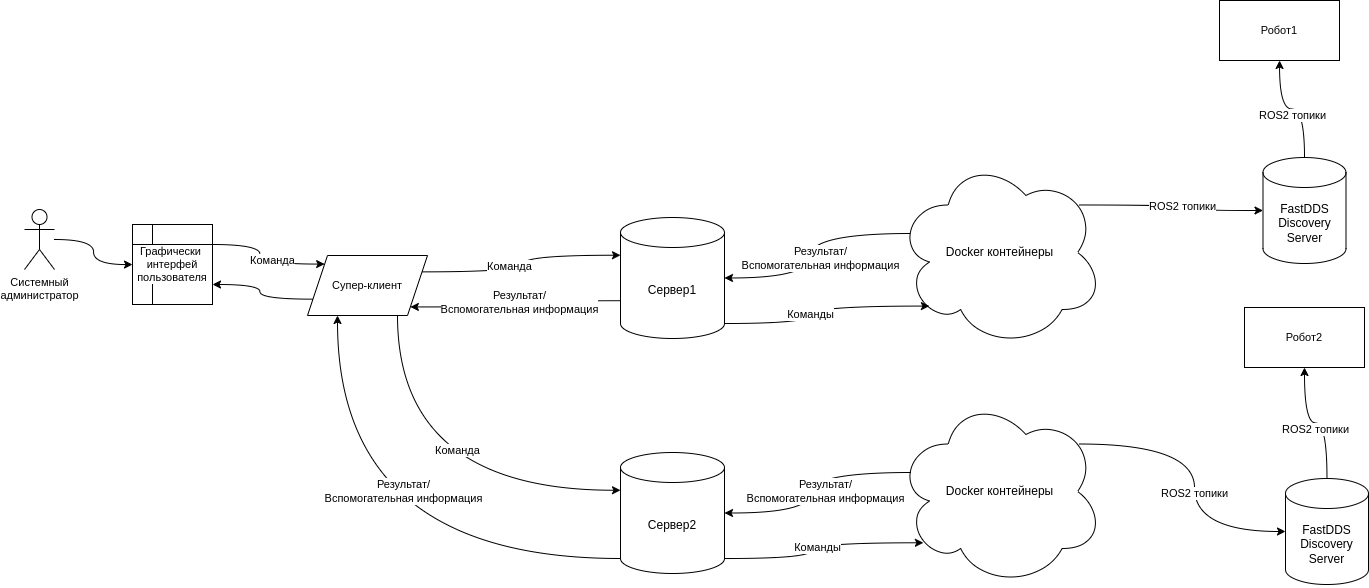
\includegraphics[scale = 0.35]{./figure/base_architure}
\caption{Схема взаимодействия компонент}
\label{fig:manip_photo}
\end{center}
\end{figure}
\par Из рисунка видно, что клиентская часть не берет на себя главные функции в сетевом сервисе, а лишь является инфраструктурным 
компонентом позволяющий пользователям легко настраивать необходимые узлы реализующие функциональность алгоритмов одновременного
картографирования и локализации. Из схемы также становится понятна расписанная выше архитектура, здесь супер-клиент и сервера, 
реализуют клиент-серверную архитектуру, а Docker контейнера реализую микросервисную архитектуру, в которой связь между микросервисами
происходит по средствам механизма топиков ROS2. Так же супер-клиентом поддержан функционал взаимодействия с несколькими серверами.
Данная схема раскрывает лишь общие моменты архитектуры сетевого сервиса, передейдем к более подробному рассмотрению отдельных 
компонентов.
\section{Архитектура системы}
\par Проектирование архитектуры играет ключевую роль при построении системы, т.к. оно обеспечивает четкое понимание структуры и 
взаимодействия всех компонентов. Проектирование архитектуры позовляет выявить возможные проблемы и оценить возможные риски, что 
способствует более эффективному управлению ресурсами и сроками разработки, кроме того, хорошо продуманная архитектура облегчает 
масштабирование и модификации системы в будущем, что особенно важно в условиях быстро меняющегося технологического мира.
\subsection{Архитектура сетевого взаимодействия}
\par Вопрос архитектуры системы хотелось бы начать с клиент серверного взаимодействия между супер-клиентом и сервером. Основой является
библиотека Boost.Asio способная поддерживать сеанс связи между клиентом и сервером и создавать асинхронные задачи связи для пересылки 
данных. Для того чтобы пересылать данные между клиентом и сервером мало одной возможности, необходимо иметь собственный протокол связи,
вариант использования готового протокола не подходит ввиду того, что такой протокол не сможет вместить в себя данные либо будет 
избыточен. Проектирование протокола связи необходимо начать с определения структур данных, которые будут пересылаться в ходе сетевого 
взаимодействия. Такого рода структуры обычно состоят из двух частей - "головы" и "тела", термины "голова" употребляется не в прямом 
значении, а в переносном, обозначая первые несколько битов в которых кодируются вспомогательные данные. Вспомогательными данными 
обычно являются длины, коды и т.п. величины, которые характеризуют данное сообщение и помогают в распозновании основные данные в "теле".
В нашем случае, удобно было бы реализовать подобную структуру в виде следующего класса:
\begin{lstlisting}[language=C++, frame=single, xleftmargin=15pt, caption={Структура данных "сообщение"},label=DescriptiveLabel]
class SerializedMessage {
public:
        enum { HeaderLength = 7 };
        
private:
        char header_[HeaderLength];
        char* data_;
        uint32_t body_length_;
};
\end{lstlisting}
\par Так как передача структуры напрямую между двумя устройствами невозможна, то для передачи необходима процедура сериализации, которая
превратит структуру данных в последовательный набор байтов. После приема данных необходима обратная сериализации процедура - десериализация,
которая позволяет из потока битов восстановить структуру данных. C++ класс продемонстрированный выше служит промежуточной структурой данных 
в процессе сериализации/дессериализации, его структура позволяет легко поддерживать этот процесс. Во-первых, "голова" структуры - поле 
header\_ имеет тип char* и является массивом из битов длины HeaderLength. Неизменяемость длины "головы" позволяет в процессе сериализации 
и дессериализации однозначно закодировать необходимые вспомогательные данные. Однозначность кодирования заключается в том, что данные 
закодированные внутри находяться в строго определенном порядке, задокументированном в протоколе. В процессе сетевого взаимодействия,
когда поток битов проходит по сети и доходит до серверной/клиентской части сетевого сервиса, в процессе десериализации будут прочитаны 
именно первы HeaderLength байт сообщения, что позволит декодировать и остальную часть сообщения, следующего после "головы". Для большей
наглядности, продемонструем процесс в виде рисунка:
\newpage
\begin{figure}[ht]
\begin{center}
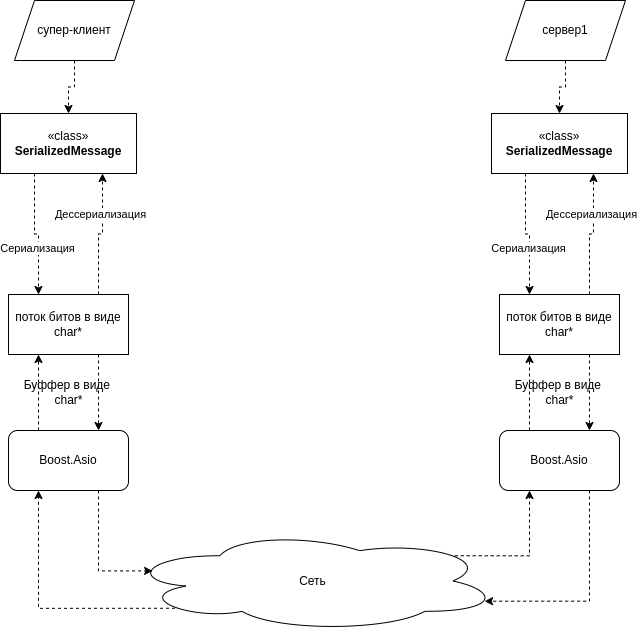
\includegraphics[scale = 0.5]{./figure/base_networking}
\caption{Схема взаимодействия компонент}
\label{fig:manip_photo}
\end{center}
\end{figure}
\par Модель взаимодействия между супер-клиентом раскрыта, однако, это не единственное сетевое взаимодействие реализованное в данной работе.
Следующий момент касается взаимодействия сервера с микросервисами на основе Docker контейнеров. Как было раскрыто в первой главе, Docker 
стостоит из нескольких частей, самой главной из которых является Docker Engine, который в свою очередь состоит из демона и утилит для 
взаимодействия с ним. Утилит всего 3-и - командный интерфейс, web API и Docker SDK. Удобнее пользоваться командным интерфейсом, однако его 
использования из другого исполняемого файла затруднительно, т.к. командный интерфейс обычно уже является конечным продуктом, не допускающим
постройку над ним дополнительной архитектуры, что приводит к тому, что из исполняемого файла можно вызвать процедуру командного интерфейса,
однако результат работы и процесс выполнения проконтролировать невозможно. Например, при попытке вызвать команду \(docker  ps\) из 
исполняемого файла, возможен вариант того, что демон Docker отключен, по той или иной причине, что приведет к тому что команда закончится 
неудачно, однако исполняемая программа никак об этом не узнает, т.к. у командного интерфейса остуствует возможности интеграции с другими 
программами. Вариант использования Docker SDK в данном случае невозможен, т.к. компания создала SDK лишь для нескольких языков, C++ к 
которым не принадлежит, остается использование web API, который предоставляет RESTful API по протоколу HTTP/HTTPS, которым может
воспользоваться абсолютно любой клиент демона, который способен отправлять ему HTTP запросы с правильной структурой.
\par\noindent \textsl{\textbf{Замечание 1:} Software Development Kit (SDK) - набор инструментов разработки программного обеспечения,
позволяющий создавать собственные решения на своей основе.}
\par\noindent \textsl{\textbf{Замечание 2:} RESTful API (полные по REST API) - стандарт поддерживающий набор правил для web API, что 
позволяет создавать удобные, хорошо поддерживаемые веб интерфейсы.}
\par Для работы с веб-интерфейсом Docker - а необходима библиотека способная отправлять HTTP запросы определенной структуры, такой 
библиотекой является \href{https://github.com/aslze/asl}{ASL}. В анализе она не упомянута, т.к. напрямую не относится к реализации 
сетевого сервиса, а лишь является компонентом другой библиотеки, реализующей простой SDK на основе веб-интерфейса Docker -
\href{https://github.com/sees1/docker_cpp}{docker\_cpp}. Часть функционала данной библиотеки была также реализована в этой работе.
У Docker Web API являющейся веб-интерфейсом существует документация, благодаря которой и был реализован данный SDK. Для большей
наглядности продемонстрируем работу сервиса с Docker демоном через веб-интерфейс ввиде рисунка:
\vspace{5mm}
\begin{figure}[ht]
\begin{center}
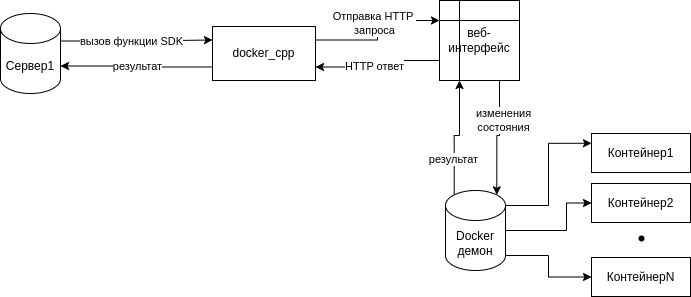
\includegraphics[scale = 0.6]{./figure/docker_connect}
\caption{Схема взаимодействия компонент}
\label{fig:manip_photo}
\end{center}
\end{figure}
\par Последней частью сетевого взаимодействия является перессылка сообщений ROS2 между микросервисами, реализованными с использованием
Docker, и перессылка сообщений между микросервисами и роботом, который является конечным потребителем обработанных сервисом данных.
ROS2 благодаря использованию DDS, может создавать связь не только между узлами на одном компьютере, но может быть использован в 
качестве сервера для пересылки сообщений между компьютерами, разберем механизм связи по порядку. Для того, чтобы Docker контейнеры 
были способы пересылать сообщения между собой необходима соответствующая настройка. Самый простой вариант, настраивать каждый из 
создающихся контейнеров на использование сети "хоста". Таким образом, каждый контейнер запущенный на "хосте" для другого устройства 
будет виден как сам "хост", что очень удобно, т.к. дает нам доступ в сеть без предварительной настройки сети контейнеров на самом 
"хосте". Следующая проблема, возникающая на пути к запуску микросервисов с выходом в сеть и межконтейнерной связью, является механизм 
распределенной памяти\cite{sharedMemArt} в ROS2. Дело в том, что по умолчанию, DDS платформа являющаяся основной ROS2 снижая нагрузку на сеть использует 
для взаимодействия между узлами распределенную память. Распределенная память является абстракцией, которая позволяет нескольким 
процессам в операционной системе иметь общую область памяти, по-умолчанию это запрещено. Такая общая память позволяет при пересылке 
не тратить процессорное время на процесс сериализации/дессериализации каждого сообщения посылаемого одним узлом другому, а просто
переместить всю структуру данных в другую облась в памяти. Проблема заключается не в самой распределенной памяти, а в том, как 
Docker использует ресурсы операционной системы для поддержания контейнеров. По-умолчанию, Docker контейнер не может взаимодействовать 
с распределенной памятью основной операционной системы, что не дает узлу запущенному внутри Docker контейнера возможность пересылать 
сообщения, однако, в Docker существует настройка, которая дает доступ. И наконец, последняя проблема, пересылка сообщений между 
разными устройствами в сети. Существует два способа создания такого взаимодействия, первый - с помощью механизма подсетей в ROS2, 
второй - с помощью механизма Discovery Server - ов. Первый механизм эффективен, когда устройств в сети немного, тогда механизм 
подсетей в ROS2, с помощью мультикастинга, помогает системе находить новые узлы объединяя подсети, однако, мультикастинг - сильно 
нагружает сеть и зачастую выходит из строя, поэтому наиболее надежным методом пересылки сообщений между микросервисами и роботом,
является механизм Discovery Server - ов. По аналогии с подобным механизмом в ROS первой версии, механизм Discovery Server создает
сервер координирующий и осуществляющий перессылку сообщений между устройствами подключенными к нему. 
\par\noindent \textsl{\textbf{Замечание 2:} Хост - в контексте компьютерных сетей и интернета означает любое уникальное устройство 
в сети имеющее собственный IP-адресс.}
\section{Архитектура графического интерфейса пользователя}
\par Архитектура графического интерфейса пользователя основывается на использовании функции одного из самых развитых кросплатформенных
фреймоврка - Qt. У Qt есть версии, в данной работе будет использован Qt пятой версии, или сокращенно - Qt5. Рассмотрение процесса 
проектирования и основных моментов архитектуры графического интерфейса пользователя необходимо начать с базового понимания работы самого
Qt фреймвора. В первую очередь, стоить заметить, что Qt5 - Объекто-Ориентированный фреймворк, что говорит нам о том, что вся основная 
функциональность в нем заключена в классах и что Qt5 - написан на C++ и большая часть его функциональности работает для этого языка 
программирования. Основные классы, который используют программисты при работе с Qt5 называются виджетами. Виджеты работают по принципу 
матрешки, позволяя вкладывать в себя другие виджеты и т.д. Это свойство виджетов позволяет строить графический интерфейс пользователя 
по принципу конструктора. Виджеты являются классами в языке C++ и у них существуют определенные ограничения на взаимодействия с другими 
классами-виджетами, поэтому создатели Qt5 предусмотрели возможные проблемы и искусственно создали рефлексию\cite{reflectArt} для собственного фреймворка.
Рефлексия - механизм, позволяющий классам получать информацию о своей структуре и поведению во время выполнения. Рефлексия в Qt5 необходим 
для создания собственного механизма связи - слотов и сигналов. Механизм слотов и сигналов схож с механизмом топиков у ROS2, суть его в 
следующем, виджет создает слоты, которые используются в качестве реакции на действие сигналов. Например, представим класс клавиша, 
у класса клавиши есть слот - OnPress, допустим мы запрограммировали нашу клавиатуру таким образом, что связали сигнал Press и 
слот OnPress, при компиляции программы и нажатии на кнопку, сработает сигнал Press, а после него и слот клавиатуры OnPress, который 
выполнит некие действия, допустим выведет на экран букву соответсвующую этой клавише. Таким образом, работает механизм слотов и сигналов,
связывая несколько виджетов сетями передачи сигналов. Стоит оговориться, что слоты и сигналы в C++ принимают форму методов и перечислений
(enum).
\par\noindent \textsl{\textbf{Замечание 2:} Кроссплатформенность - свойство Программного Обеспечения (ПО) работать на нескольких программных 
платформах, так называемых, операционных системах (ОС).}
\par Центральным виджетом будет специальный вид виджетов, помогающий в объединений функциональности небольших приложений - MainWindow
виджет, который является более абстрактным виджетом по сравнению с другими. Он берет на себя часть процессов по управлению другими 
виджетами, он создает верхнеуровневое меню, пустое окно приложений и имеет пустой главный виджет, который можно заполнить другими.
Проще всего заполнить главный виджет с помощью менеджеров компоновки, так называемых Layout - ов, которые размещают вспомогательный виджеты 
в заданном порядке, обычно горизонтально или вертикально, еще есть вариант размещение в сетку. В данном решении, менеджер компоновки будет
вертикальным, всего виджетов главного менеджера компоновки будет два, первый виджет, находящийся сверху, будет отображать либо информацию о
текущих серверах, к которым подключен данный супер-клиент, либо информацию о микросервисах запущенных, на выбранном из перечня, сервере,
второй виджет будет отображать контекстную текстовую информацию, например о записях собранных с терминала микросервиса.
\begin{figure}[ht]
\begin{center}
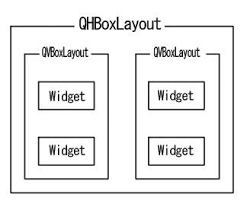
\includegraphics[scale = 0.6]{./figure/layout_examp}
\caption{Различные менеджеры компоновки}
\label{fig:manip_photo}
\end{center}
\end{figure}
\par Для создания первого главного виджета необходимо использовать изменение внешнего вида виджета, т.к. смена вид необходима нам для 
смены отображающейся информацию о серверах и информации о микросерверах. Изменять облик может специальный тип виджета, называемых
stack (от англ. - куча) виджетом, подобно анимированным рекламным банерам на улицах городов, он способен менять свой внешний вид в
зависимости от действий пользователя. С помощью данного виджета, можно будет реализовать мехнику "проваливания" внуть сервера. При
установлении соединения супер-клиента и сервера, наш графический интерфейс пользователя отобразит имя сервера и его порядковый номер на
одном из видов stack виджета, однако, если пользователь решит нажать на надпись, обозначающую имя сервера, то stack widget изменит 
свой вид и станет виджетом отображающим состояния микросервисов на данном сервере. Это и есть механика "проваливания".
\par Как говорилось раннее, центральный виджет, будет создавать также меню верхнего уровня. Так как графический интерфейс пользователя
связан с супер-клиентом, то логичным будет добавить в меню верхнего уровня возможность подключения к серверам.
\begin{figure}[ht]
\begin{center}
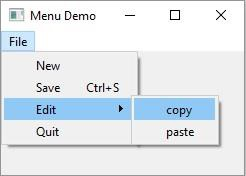
\includegraphics[scale = 0.6]{./figure/menu_examp}
\caption{Пример меню верхнего уровня}
\label{fig:manip_photo}
\end{center}
\end{figure}
\par При инициировании создании сервера через меню верхнего уровня, необходимым будет создания диалогового окна, позволяющего
пользователю супер-клиента ввести необходимый ip-адрес и порт сервера чтобы установить с ним соединение.
\begin{figure}[ht]
\begin{center}
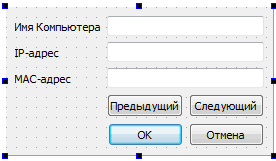
\includegraphics[scale = 0.6]{./figure/dialog_examp}
\caption{Пример диалогового окна}
\label{fig:manip_photo}
\end{center}
\end{figure}
\par После завершения процедуры подключения супер-клиента к серверу, как говорилось выше, необходимо отразить состояние микросервисов,
предназначенныех для запуска алгоритмов одновременного картографирования и локализации. Так как микросервисы в работе будут построены
на основе Docker, необходимо учитывать аспекты связанные с этим. Поскольку сетевой сервис предпологает легкую настройку сервера для 
работы с алгоритмами, то необходимо добавить возможность работать с еще не собранными контейнерами в виде Dockerfile. Таким образом
на сервере, для создания всей инфраструктуры из микросервисов потребуется хранить лишь один Dockerfile с инструкциями по сборке.
Кроме того, после сборки необходимо отображать уже собранные контейнеры, которые готовы к запуску. Само собой необходимо учитывать и 
информацию о уже запущенных контейнерах. Это подводит нас к тому что, мы должны создать 3 виджета, отображающих полную информацию о 
состояниях готовности микросервисов - не собран, собран, запущен, также нам необходимо построить структуру работы с Dockerfile и launch 
файлами, поскольку именно они буду создавать и запускаться в микросервисах.
\begin{figure}[ht]
\begin{center}
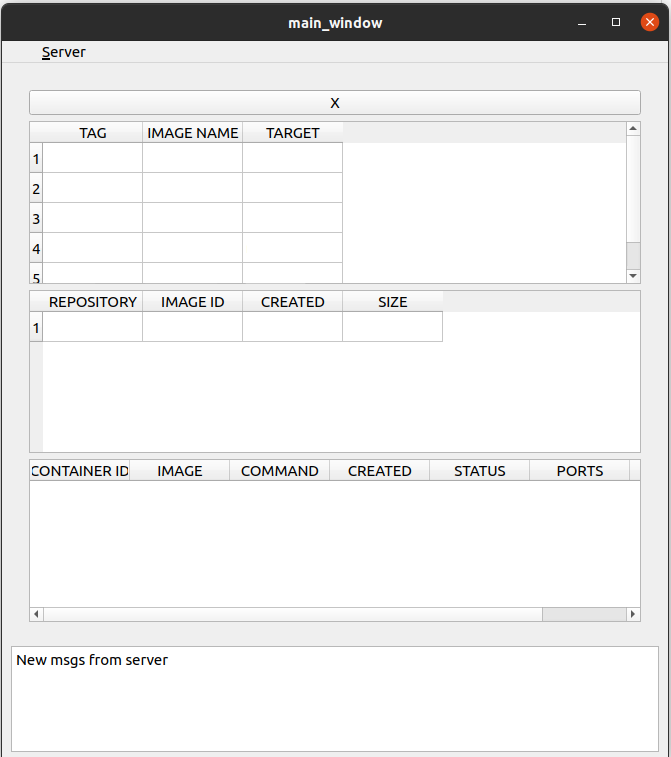
\includegraphics[scale = 0.4]{./figure/app_examp}
\caption{Пример работы с возможностями микросервисов}
\label{fig:manip_photo}
\end{center}
\end{figure}
\par В первом из трех виджетов, призванных отражать информацию о микросервисах, будет хранится информация из некоего текстового файла,
хранящегося на сервере. В данном файле, должна быть отражена информация о микросервисах, которые можно собирать и использовать, кроме 
того для создания микросервисов необходимо вручную формировать .tar.gz архив в который необходимо добавлять Dockerfile. Это необходимо,
т.к. создание контейнеров в Docker с использованием Web API невозможно напрямую с Dockerfile, необходимо посылать демону Docker через 
API специализированный запрос вместе с сериализованным .tar.gz архивом, только в этом случае он способен собрать образ контейнера.
Кроме .tar.gz, файла с перечнем образов, Dockerfile необходимых в процессе создания микросервисов, нам необходимо создать инфраструктуру 
для запуска этих микросервисов, т.к. они используют ROS2 возможности, то и запускать в автоматическом режиме их проще всего с помощью
launch файлов. Каждый из контейнеров будет запускать launch файлы, которые, в свою очередь, будут запускать определенные узлы
необходимые для корректной работы алгоритмов одновременного картографирования и локализации. Это достаточно распространненая практика 
среди компании строяющих свои робототехнические продукты, облегчающая их масштабирование. Для реализации подобной структуры лучше всего 
подходят директории компьютера. Примерная структура директорий показана на рисунке ниже:
\begin{figure}[ht]
\begin{center}
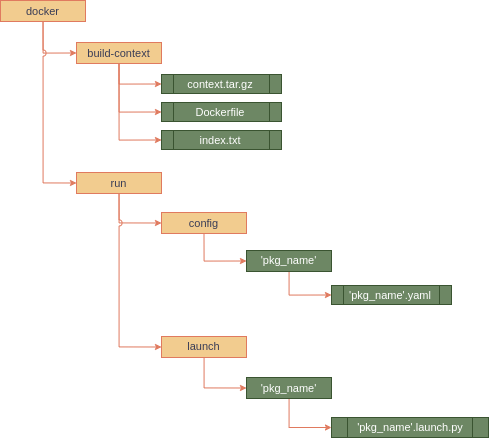
\includegraphics[scale = 0.6]{./figure/docker_folder_schema}
\caption{Структура файлов для обслуживания микросервисов}
\label{fig:manip_photo}
\end{center}
\end{figure}
\subsection{Диаграмма классов UML}
\par Unified Modeling Language (UML) - стандартный язык моделирования, используемый для визуализации, спецификации и документирования 
программных систем. В языке есть набор графические диаграмм, которые позволяют отразить различные стороны архитектуры приложений. 
Для создания архитектуры сетевого сервиса, в процессе работы была создана диаграмма классов UML, которая представляет собой структуру 
системы, отображающая классы и их внутренее устройство, а также связи между ними. Диаграмма классов для данного решения проблематично 
разместить в работе, поэтому необходимо разбиение общей диаграммы на несколько слабозависимых частей. Первая часть диаграммы затрагивает 
устройство обработки запросов в клиент-серверной связи, она представлена ниже:
\begin{figure}[ht]
\begin{center}
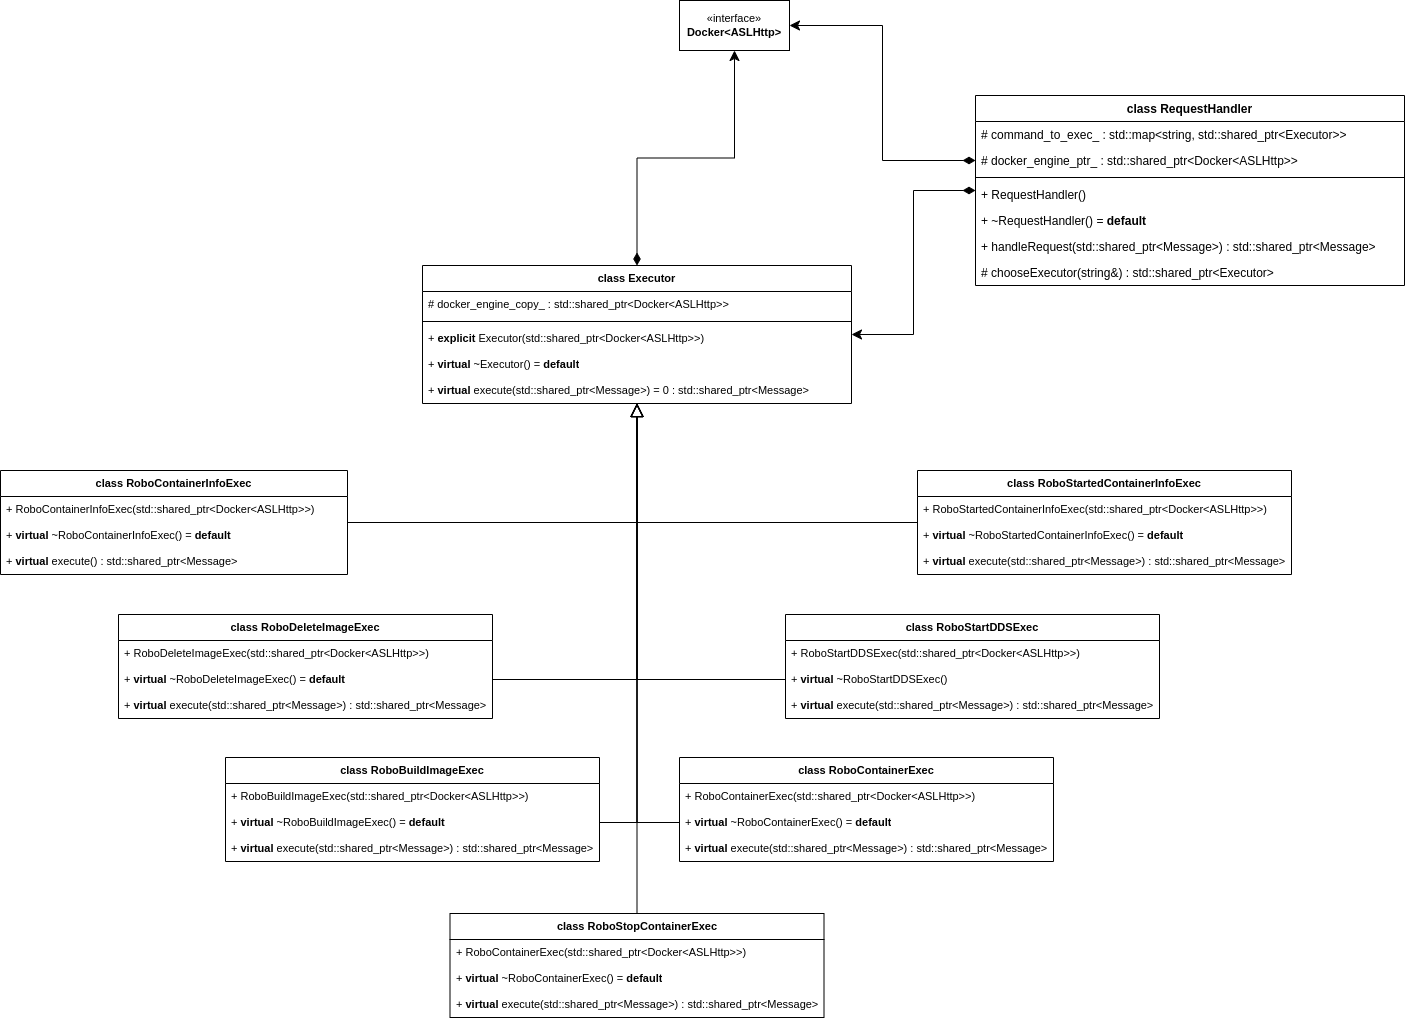
\includegraphics[scale = 0.33]{./figure/client-serv-UML}
\caption{Обработка запросов сервера}
\label{fig:manip_photo}
\end{center}
\end{figure}
\par Данная часть отражает работу функционала ответсвенного за обработку дессериализованных запросов от супер-клиента к серверу. 
Здесь класс RequestHandler получает запрос и переедадрессует его одному из классов-наследников класса Executor, ответственного за 
исполнения запросов. Внутри классов-насследников Executor - а, находятся вызов функции docker\_cpp библиотеки, которая реализует 
С++ API для вызова функции Web API Docker. Результат выполнения функций валидируется, в случае успешного выполнения обратно 
формируется сообщение-ответ на запрос, в котором находятся необходимые сведения. В случае неудачи, классы-наследники Executor 
так же формируют сообщение, отражающее причину ошибки и отправляют ее супер-клиенту, который обрабатывает ее и выдает результат.
Вторая часть данной диаграммы отражает устройство сетевого взаимодействие серверной и клиенской части сетевого сервиса:
\newpage
\begin{figure}[ht]
\begin{center}
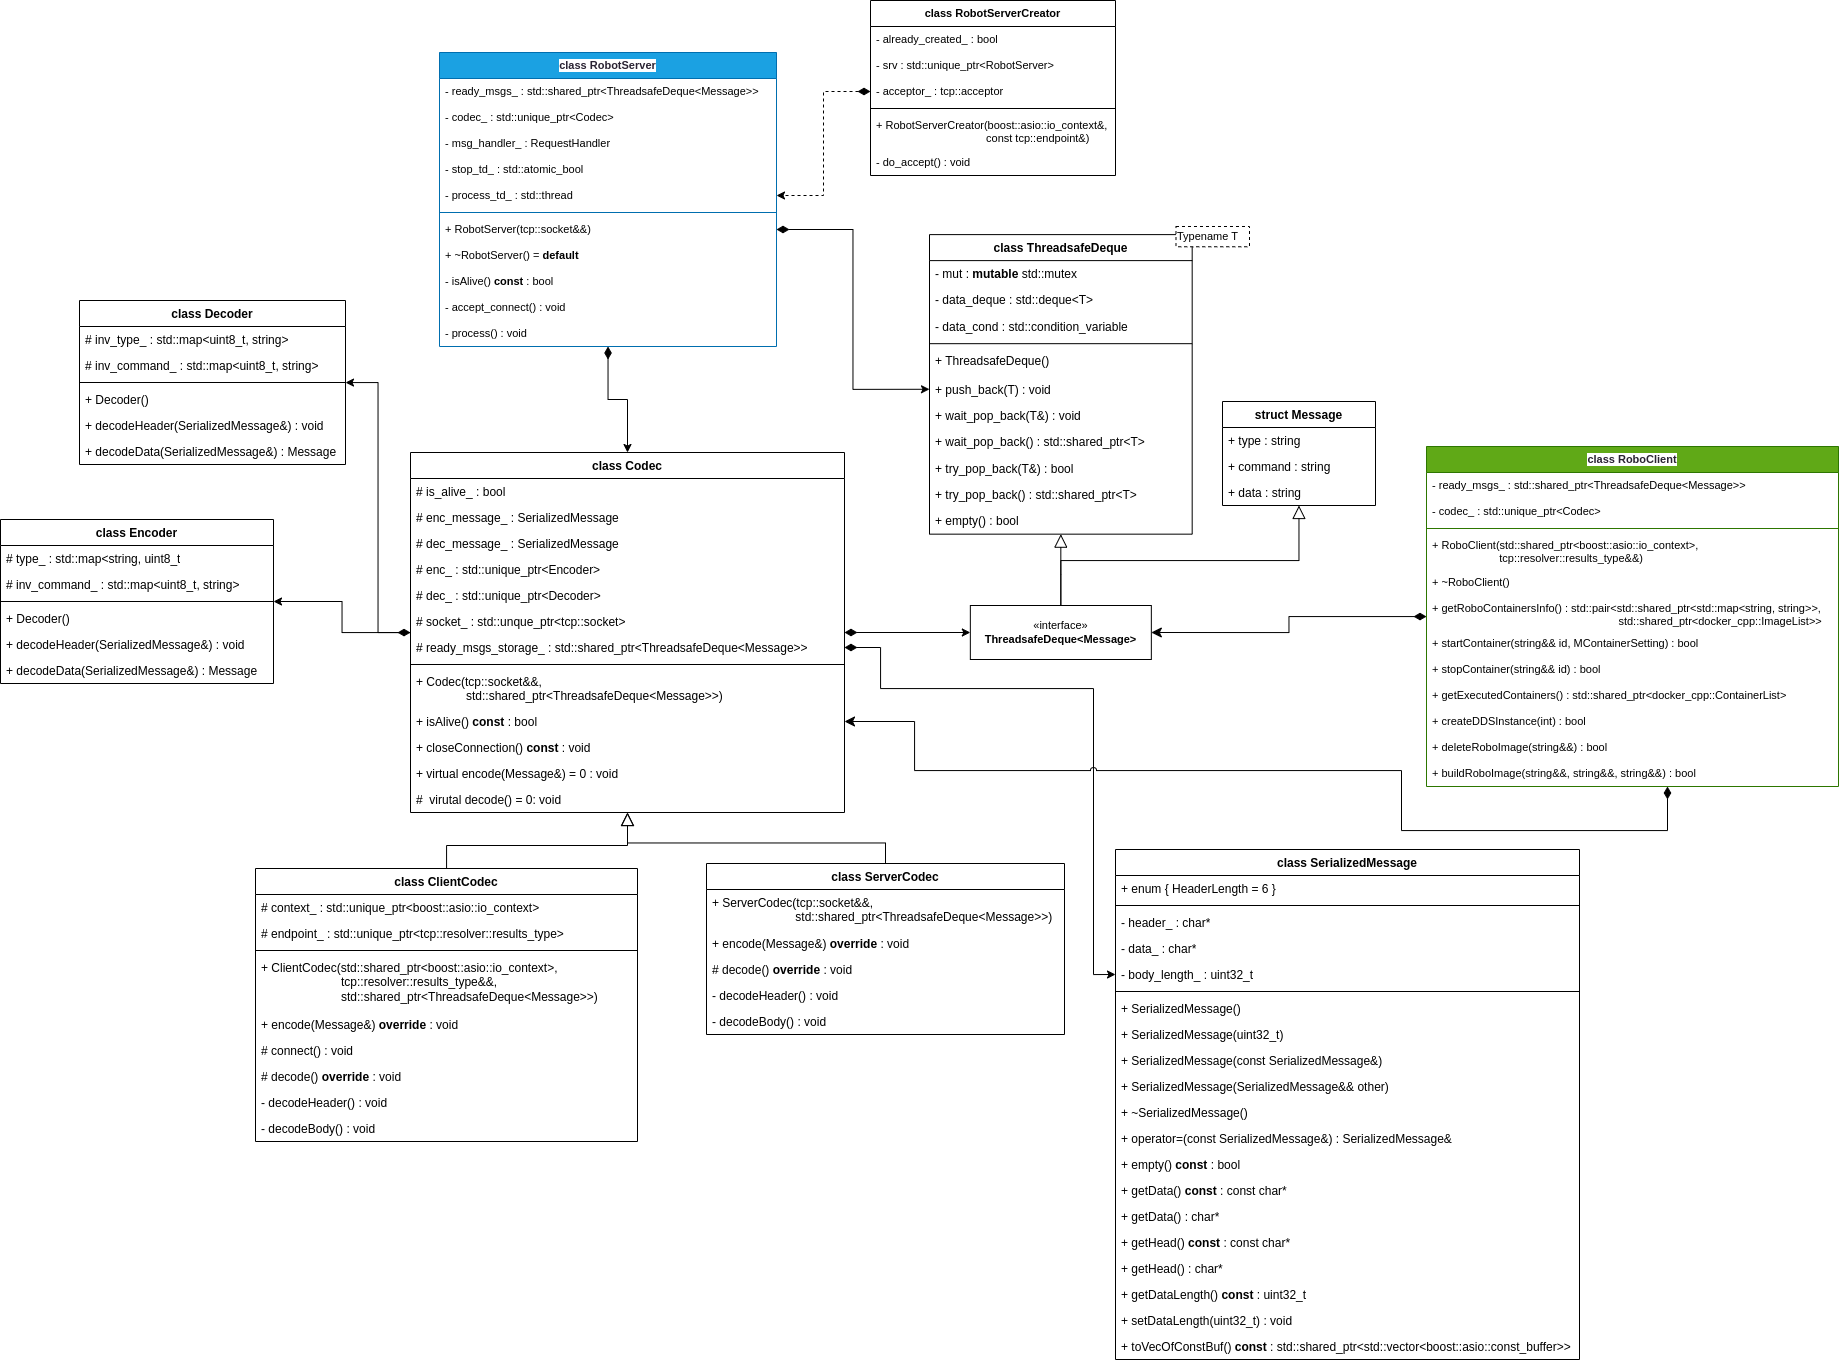
\includegraphics[scale = 0.265]{./figure/client-serv-comm}
\caption{Cетевое взаимодействия сервера и супер-клиента}
\label{fig:manip_photo}
\end{center}
\end{figure}
\par Как видно из диаграммы классы реализующие абстракции сервера и супер-клиента построенны на базе класса Codec, который реализует 
само сетевое взаимодействие на основе библиотеки Boost.Asio. Класс Codec - базовый класс для ClientCodec и ServerCodec, каждый из 
которых имеет свои отличительные особенности, помогающие им в реализации функционала связи. Так же есть классы SerializedMessage, о 
которых было кратко написано выше, и класс Message, эти классы реализуют абстракции сериализованного и дессериализованного сообщения,
а сам процесс происходит внутри классов Decoder и Encoder, которые переводят информацию между двумя классами сообщений. Процесс обработки 
запроса и подготовки ответа требует многопоточности. Многопоточность здесь разделена между классами RobotServer, реализующего 
сервер, и классом Codec равно как и между классом RoboClient и Codec. Для отправки сообщения, сервер или клиент формирует его внутри
методов своего класса, однако для того, чтобы принять и обработать сообщение, ему необходимо ждать неопределенное время. Для работы 
с неопределенным временем существует класс ThreadsafeDeque, являющийся потокобезопастной структурой данных, которая синхронизирует 
классы сервера или клиента и классы-наследники класса Codec. Во время передачи сервером или клиентом запроса в виде сообщения в метод 
encode класса Codec, они должны использовать метод push\_back класса ThreadsafeDeque, в котором, спустя время будет сформирован 
ответ, таким образом, во время вызова метода push\_back из класса RobotServer или RoboClient поток выполнения в них блокируется внутренним 
мьютексом принадлежащем ThreadsafeDeque. Как только ответ придет, классом Codec к экземпляру класса ThreadsafeDeque, который она разделяет
с RobotServer или RoboClient, будет добавлено дессериализованное сообщение и поток выполнения вновь вернется в классы сервера или клиента.
Третья и последняя часть диаграммы отражает структуру графического интерфейса пользователя принадлежащего клиентской части сетевого сервиса:
\par\noindent \textsl{\textbf{Замечание 2:} Потокобезопастность - свойство структур данных, позволяющее им работать с несколькими 
программными потоками, не вызывая опасных состояний гонки или взаимоблокировки.}
\begin{figure}[ht]
\begin{center}
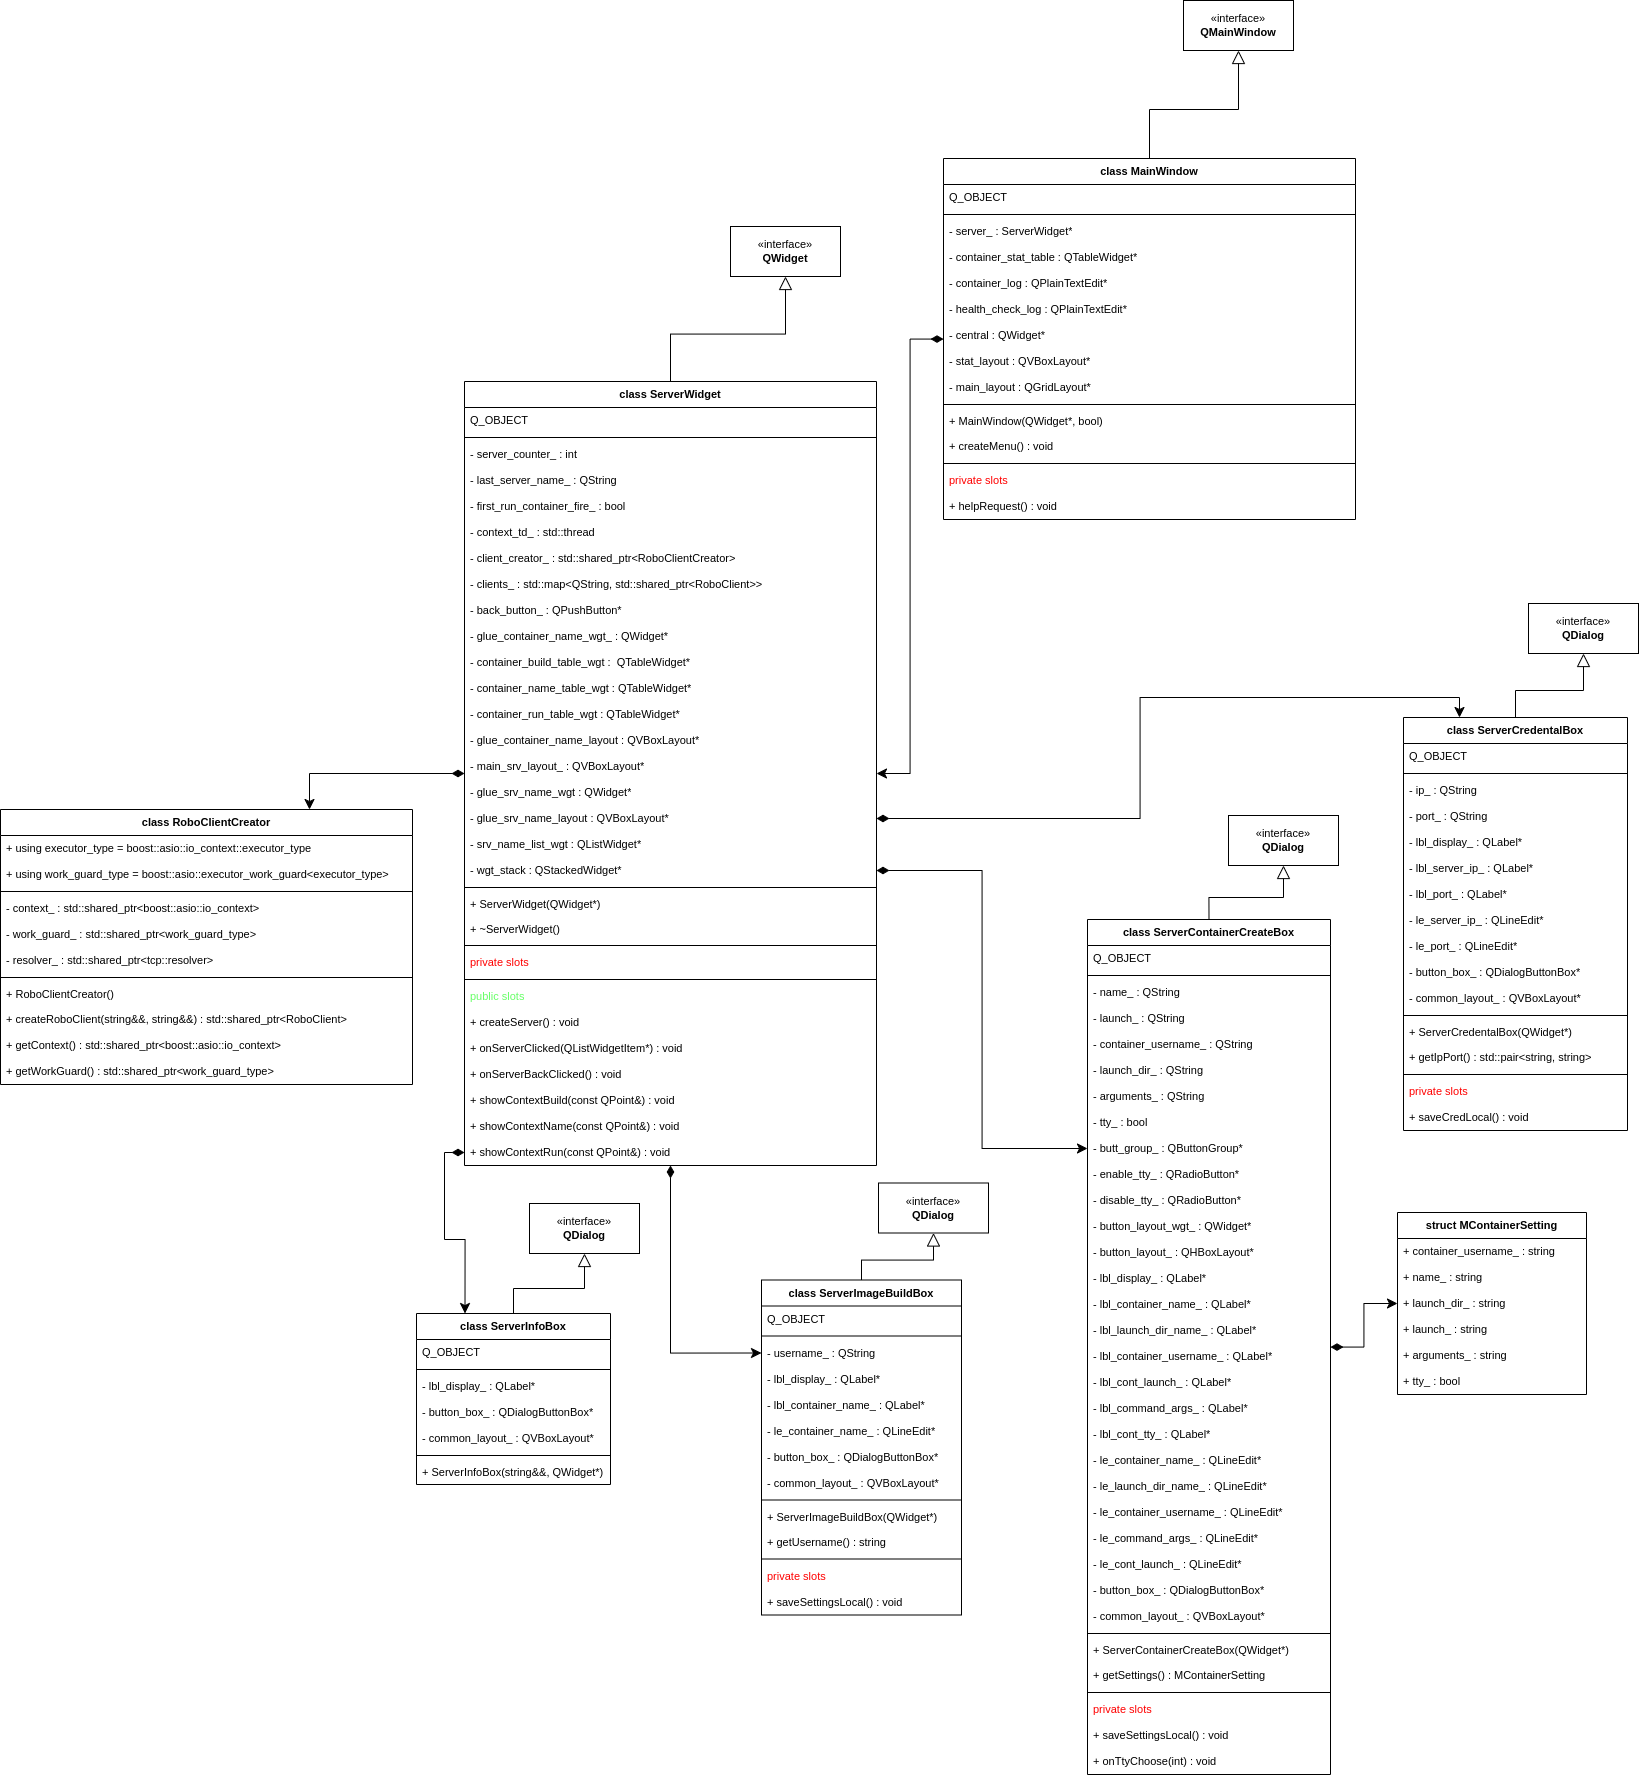
\includegraphics[scale = 0.265]{./figure/gui_uml}
\caption{Графический интерфейс пользователя}
\label{fig:manip_photo}
\end{center}
\end{figure}
\par В данной схеме находится класс MainWidget, о котором говорилось выше, в части про архитектуру графического интерфейса. Он содержит 
в себе главного менеджера компоновки, который добавляет в себя классы-виджеты ServerWidget использующий stack виджет для реализации 
функциональности управления серверами и микросервисами, а также QPlainTextEdit виджет, который способен отображать текстовую информацию.
ServerWidget в свою очередь содержит управление созданием класса супер-клиента реализованого в виде класса RoboClientCreator, а также 
класы ServerInfoBox, ServerImageBuildBox, ServerContainerCreateBox и ServerCredentialBox, которые управляют всплывающими окнами, 
информирующими пользователя о различных произошедших ситуациях или требующих от пользователя ввода данных. Например, класс 
ServerCredentialBox является всплывающим окном, которое отображается в случае добавления пользователем нового сервера и требующем от 
пользователя данных необходимых для подключение - ip-адресса и порта.
\chapter{Реализация сетевого сервиса}
\par В данной главе будут показаны основные моменты реализации сетевого сервиса с примерами из программного кода решения. Также будут 
затронуты моменты касающиеся особенностей использования функции библиотек для сетевого взаимодействия и создания графического интерфейса.
\section {Разработка сетевого взаимодействия}
\par Сетевое взаимодействие, как было написано ранее, является ключевой механикой данной работы. Практически все взаимодействие между 
компонентами сетевого сервиса происходит с использованием сетевых технологий. Вопрос выбора библиотек для реализации сетевого
взаимодействия, был рассмотрен в первой главе данной работы, в ходе которого стало очевидным преимущество библиотеки Boost.Asio для 
создания подобного рода системы. Хотелось бы начать с рассмотрения протокола для сетевого взаимодействия, процесса
сериализации/дессериализации и создания асинхронных задач связи.
\subsection{Cоздания инфраструктуры связи}
\par Прежде чем начать обмен данными между устройствами в сети, необходимо наладить инфраструктур, которая будет отвечать за установку 
и поддержку этого взаимодействия. Рассмотрим класс RobotServerCreator ответсвенный за начало сетевого взаимодействия. Он также реализует 
функции создания сервера:
\begin{lstlisting}[language=C++, frame=single, xleftmargin=15pt, caption={Заголовочный файл класса RobotServerCreator},label=DescriptiveLabel]
class RobotServerCreator {
        public:
                RobotServerCreator(boost::asio::io_context& io_context, const tcp::endpoint& endpoint);
                ~RobotServerCreator();
                
        private:
                void do_accept();
                
        private:
                bool already_created_;
        
                std::unique_ptr<RobotServer> srv;
                tcp::acceptor acceptor_;
        };
\end{lstlisting}
\begin{lstlisting}[language=C++, frame=single, xleftmargin=15pt, caption={Определение методов класса RobotServerCreator},label=DescriptiveLabel]
RobotServerCreator::RobotServerCreator(boost::asio::io_context& io_context, const tcp::endpoint& endpoint)
: already_created_(false),
        acceptor_(io_context, endpoint)
{
        do_accept();
}

RobotServerCreator::~RobotServerCreator()
{
        if (srv != nullptr)
        srv->shutdown();
        srv.reset();
}

void RobotServerCreator::do_accept() {
        acceptor_.async_accept([this](boost::system::error_code ec, tcp::socket socket) {
        if(!ec && !already_created_)
        {
        srv = std::make_unique<RobotServer>(std::move(socket));
        already_created_ = true;
        }

        do_accept();
        });
}
\end{lstlisting}
\par Из заголовочного файла видно, что класс использует std::unique\_ptr<RobotServer> для хранения экземпляра класса, реализующего сервер.
Это необходимо для того, чтобы недопустить создание нового объекта этого класса, т.к. должен поддерживаться инвариант существования 
только одного сервера на компьютере. Конструктор класса принимает ссылки на объекты классов boost::asio::io\_context и
boost::asio::ip::tcp::endpoint. Объект класса boost::asio::io\_context реализует программную сущность позволяющую осуществлять перессылку 
сообщений, являясь основным классом библиотеки Boost.Asio для поддержания асинхронной передачи данных. Класс boost::asio::ip::tcp::endpoint
является реализацией структуры данных, ответсвенной за хранения учетных данных сервера, таких как ip-адресс и порт. В конструкторе эти 
данные используются для создания сущности boost::asio::ip::tcp::acceptor, которая принимает входящие подключения к серверу. Далее идет 
вызов метода do\_accept, внутри которого используется метод объекта accetor\_, являющегося менеджером подключений, функция которого 
заключается в установлении соедниения с клиентом. В случае успеха, создается объект boost::asio::ip::tcp::socket, который является 
абстракцией сетевого соединения. В дальнейшем, с помощью данного сетевого сокета станет возможным передача данных между устройствами в 
сети. Также, в случае успешной установки сетевого соединения, вызывается лябмда-функция, переданная методу async\_accept, внутри которой 
реализована проверка факта создания сервера, если проверка пройдена, то создается новый сервер. 
\par Почти идентичным, за исключением пары моментов, является создание инфраструктуры связи с клиентской стороны сервиса.
\begin{lstlisting}[language=C++, frame=single, xleftmargin=15pt, caption={Заголовочный файл класса RoboClientCreator},label=DescriptiveLabel]
class RoboClientCreator {
        public:
                using executor_type = boost::asio::io_context::executor_type;
                using work_guard_type = boost::asio::executor_work_guard<executor_type>;
        public:
                RoboClientCreator();
        
                std::shared_ptr<RoboClient> createRoboClient(std::string& ip,std::string& port);
                std::shared_ptr<boost::asio::io_context> getContext();
                std::shared_ptr<work_guard_type> getWorkGuard();
        
        private:
                std::shared_ptr<boost::asio::io_context> context_;
                std::shared_ptr<work_guard_type> work_guard_;
                std::shared_ptr<tcp::resolver> resolver_;
        };
\end{lstlisting}
\begin{lstlisting}[language=C++, frame=single, xleftmargin=15pt, caption={Определение методов класса RoboClientCreator},label=DescriptiveLabel]
RoboClientCreator::RoboClientCreator()
: context_(std::make_shared<boost::asio::io_context>()),
  work_guard_(std::make_shared<work_guard_type>(boost::asio::make_work_guard(*context_))),
  resolver_(std::make_shared<tcp::resolver>(*context_))
{ }

std::shared_ptr<RoboClient>
RoboClientCreator::createRoboClient(std::string& ip, std::string& port)
{
        auto&& endpoint = resolver_->resolve(ip.c_str(), port.c_str());

        return std::make_shared<RoboClient>(context_, std::move(endpoint));
}

std::shared_ptr<boost::asio::io_context>
RoboClientCreator::getContext()
{
        return context_;
}

std::shared_ptr<RoboClientCreator::work_guard_type>
RoboClientCreator::getWorkGuard()
{
        return work_guard_;
}
\end{lstlisting}
\par Поговорим про различия, для клиентов разрешено создание нескольких экземпляров класса RoboClient реализующего функциональность 
клиента, т.к. мы должны поддерживать инвариант, позволяющий одному супер-клиенту взаимодействовать с несколькими серверами сразу.
Для создания одного из клиентов, необходимо использовать учетные данные, такие как ip-адресс и порт сервера, к которому подключается 
данный клиент, эти данные в методе createRoboClient мы передаем объекту resolver\_, являющимся объектом класса boost::asio::ip::tcp::resolver,
суть которого преобразование адресса сервера в ip-адресс используя DNS сервер. Грубо говоря, это перевод адреса, заданного с помощью 
строковых литералов в ip-адрес, заданный с помощью цифр и точек. Результатом работы метода данного объекта, является tcp::endpoint, 
который, как говорилось ранее, хранит учетные данные подключения. Также стоит отметить тот факт, что пересылка данных возможна лишь 
после вызова метод run() объекта класса boost::asio::io\_context. Данная операция является блокирующей, она останавливает поток управления,
что приводит к невозможности выполнения программных инструкций следующих ниже по коду. Это создает проблему в графическом интерфейсе пользователя,
т.к. именно в классе ServerWidget, отвественным за реализацию графических отображений управления, идет работа с группой созданных объектов 
класса RoboClient. Такая проблема вынуждает создавать отдельный поток для использования метода run() объекта класса boost::asio::io\_context.
\par Данный классы являются лишь "фабрикой" для создания объектов клиента и сервера. Они выступают в качестве объектов хранящих разделяемое 
клиентами и серверами состояния. В данном случае, они хранят boost::asio::io\_context и т.п. вещи, которые являются общими для всех объектов 
клиентов и серверов. Манипуляцией потоками данных, в данном случае, занимаются классы реализующие клиент и сервер.
\par Рассмотрим реализацию сервера:
\begin{lstlisting}[language=C++, frame=single, xleftmargin=15pt, caption={Заголовочный файл класса RobotServer},label=DescriptiveLabel]
class RobotServer {
        public:
                RobotServer(tcp::socket&& socket);
                ~RobotServer();
        
                void shutdown();
        
        private:
                void isAlive();
                void accept_connect();
                void process();
        
        private:
                std::shared_ptr<ThreadsafeDeque<Message>> ready_msgs_;
                std::unique_ptr<Codec> codec_;
        
                RequestHandler msg_handler_;
        
                std::atomic_bool stop_td_;
                std::thread process_td_;
};
\end{lstlisting}
\begin{lstlisting}[language=C++, frame=single, xleftmargin=15pt, caption={Определение методов класса RobotServer},label=DescriptiveLabel]
RobotServer::RobotServer(tcp::socket&& socket)
: ready_msgs_(std::make_shared<ThreadsafeDeque<Message>>()),
  codec_(std::make_unique<ServerCodec>(std::move(socket), ready_msgs_)),
  stop_td_(false)
{
        process_td_ = std::thread(&RobotServer::process, this);
}

void RobotServer::shutdown() {
        stop_td_ = true;
        ready_msgs_->shutdown();

        if (process_td_.joinable())
        {
                process_td_.join();
        }

        codec_->closeConnection();
}

RobotServer::~RobotServer() {
        ready_msgs_.reset();
        codec_.reset();
}

void RobotServer::process() {
        while(!stop_td_)
        {
                std::shared_ptr<Message> request = ready_msgs_->wait_pop_back();

                if (request != nullptr)
                {
                        std::shared_ptr<Message> resp = msg_handler_.handleRequest(request);
                        codec_->encode(*resp);
                }
        }
}

void RobotServer::isAlive() {
        if (!codec_->isAlive())
        {
                stop_td_ = true;
                throw std::runtime_error("Our connection to client is die,
                 terminate RobotServer!");
        }
}
\end{lstlisting}
\par В конструкторе, абстракция сервера, реализованного в виде класса RobotSever, создает объект класса std::shared\_ptr<ThreadsafeDeque<Message>>,
являющегося одновременно хранилищем
для сообщений-ответов и структурой, синхронизирующей процесс запрос-ответ. Так же в конструкторе создается объект класса 
std::shared\_ptr<ServerCodec>, принимающий сокет и хранилище, необходимый для управления сетевым взаимодействием. Внутри конструктора 
создается объект std::thread, которому передается метод класса и указатель на этот класс, в котором происходит основная логика процесса 
запрос-ответ. В цикле проверяющем условие остановки сервиса, реализованном на атомарном типе bool, с помощью объека stop\_td\_, приосходит 
ожидание сервером запроса, реализованого в форме вызова метода wait\_pop\_back() хранилища. Как уже было упомянуто, данное хранилище 
выступает в роли структуры данных синхронизирующей процесс запрос-ответ, путем приостановки потока выполнения на методе wait\_pop\_back(),
который является блокирующим. Синхронизация принимает форму блокировки потока, т.к. состояния гонки в функции невозможны, однако возможны
большие накладные расходы ресурсов на работу цикла сервера в "холостую". Таким образом сервер "дожидается" запроса на действия от
супер-клиента. После отправки супер-клиентом запроса,
происходит разблокировка потока выполнения и переход к следующим инструкциям, которые формируют "ответ" сервера. Формирование "ответа" 
происходит с использованием функций класса RequestHandler, однако, это выходит за рамки реализации задачи сетевого взаимодейсвия и будет 
рассмотрено в дальнейшем. Рассмотрим реализацию клиента:
\begin{lstlisting}[language=C++, frame=single, xleftmargin=15pt, caption={Заголовочный файл класса RoboClient},label=DescriptiveLabel]
class RoboClient {
        public:
                RoboClient(std::shared_ptr<boost::asio::io_context> context,
                           tcp::resolver::results_type&& endpoint);
                ~RoboClient();
        
                std::pair<std::shared_ptr<std::map<std::string, std::string>>,
                          std::shared_ptr<docker_cpp::ImageList>>
                getRoboContainersInfo();
                bool startContainer(std::string&& id, MContainerSetting settings);
                bool stopContainer(std::string&& id);
                std::shared_ptr<docker_cpp::ContainerList> getExecutedContainers();
                bool createDDSInstance(int id);
                bool deleteRoboImage(std::string&& id);
                bool buildRoboImage(std::string&& name, std::string&& target, std::string&& username);
                bool getRoboLog(std::string&& id, std::string& log);
        
        private:
                std::shared_ptr<ThreadsafeDeque<Message>> ready_msgs_;
        
                std::unique_ptr<Codec> codec_;
};
\end{lstlisting}
\begin{lstlisting}[language=C++, frame=single, xleftmargin=15pt, caption={Определение методов класса RoboClient},label=DescriptiveLabel]
RoboClient::RoboClient(std::shared_ptr<boost::asio::io_context> context,
                       tcp::resolver::results_type&& endpoint)
: ready_msgs_(std::make_shared<ThreadsafeDeque<Message>>()), 
  codec_(std::make_unique<ClientCodec>(context, std::move(endpoint), ready_msgs_))
{ }

RoboClient::~RoboClient()
{
        codec_->closeConnection();
}

std::pair<std::shared_ptr<std::map<std::string, std::string>>,
          std::shared_ptr<docker_cpp::ImageList>>
RoboClient::getRoboContainersInfo()
{
        Message msg;
        msg.type = "Request";
        msg.command = "getRoboContainerInfo";
        msg.data = "";

        codec_->encode(msg);

        std::shared_ptr<Message> resp = ready_msgs_->wait_pop_back();

        if (resp->result)
        {
                size_t delim = resp->data.find(" ");
                std::string tag_map = resp->data.substr(0, delim);
                std::string image_info_list = resp->data.substr(delim + 1);

                json m = json::parse(tag_map);
                json im = json::parse(image_info_list);
                return {std::make_shared<std::map<std::string, std::string>>(
                                m.get<std::map<std::string, std::string>>()),
                        std::make_shared<docker_cpp::ImageList>(
                                im.get<std::vector<docker_cpp::ImageInfo>>())};
        }
        else
        {
                std::cerr << resp->data << std::endl;
                return {nullptr, nullptr};
        }
}

bool RoboClient::startContainer(std::string&& id,  MContainerSetting settings)
{
        Message msg;
        msg.type = "Request";
        msg.command = "execRoboContainer";

        docker_cpp::CreateConfig conf;

        conf.Image = id.substr(7);
        conf.Tty = settings.tty_;
        conf.OpenStdin = true;
        conf.NetworkDisabled = false;
        conf.Entrypoint.push_back("bash");
        conf.Entrypoint.push_back("-c");
        std::string command = settings.launch_dir_ + ".launch.py " + settings.arguments_;
        conf.Cmd.push_back(command);
        conf.hostConfig.networkMode = "host";
        conf.hostConfig.autoRemove = false;
        conf.hostConfig.privileged = true;
        conf.hostConfig.ipcMode = "host";
        conf.hostConfig.readonlyRootfs = false;

        json j = conf;

        msg.data = settings.launch_dir_ + " " + settings.name_ + " " + j.dump();

        codec_->encode(msg);

        std::shared_ptr<Message> resp = ready_msgs_->wait_pop_back();

        if (!resp->result)
        {
                std::cerr << resp->data << std::endl;
                return false;
        }

        return true;
}

bool RoboClient::stopContainer(std::string&& id)
{
        Message msg;
        msg.type = "Request";
        msg.command = "stopRoboContainer";
        msg.data = std::move(id);

        codec_->encode(msg);

        std::shared_ptr<Message> resp = ready_msgs_->wait_pop_back();

        if (!resp->result)
        {
                std::cerr << resp->data << std::endl;
                return false;
        }

        return true;
}

std::shared_ptr<docker_cpp::ContainerList> RoboClient::getExecutedContainers()
{
        Message msg;
        msg.type = "Request";
        msg.command = "getExecutedRoboContainer";
        msg.data = "";

        codec_->encode(msg);

        std::shared_ptr<Message> resp = ready_msgs_->wait_pop_back();

        if (resp->result)
        {
                json j = json::parse(resp->data);
                return std::make_shared<docker_cpp::ContainerList>(
                        j.get<std::vector<docker_cpp::ContainerInfo>>());
        }
        else
        {
                std::cerr << resp->data << std::endl;
                return nullptr;
        }
}

bool RoboClient::createDDSInstance(int id)
{
        Message msg;
        msg.type = "Request";
        msg.command = "execDDSServer";
        msg.data = std::to_string(id);

        codec_->encode(msg);

        std::shared_ptr<Message> resp = ready_msgs_->wait_pop_back();

        if (!resp->result)
        {
                std::cerr << resp->data << std::endl;
                return false;
        }

        return true;
}

bool RoboClient::deleteRoboImage(std::string&& id)
{
        Message msg;
        msg.type = "Request";
        msg.command = "deleteRoboImage";
        msg.data = id.substr(7);

        codec_->encode(msg);

        std::shared_ptr<Message> resp = ready_msgs_->wait_pop_back();

        if (!resp->result)
        {
                std::cerr << resp->data << std::endl;
                return false;
        }

        return true;
}

bool RoboClient::buildRoboImage(std::string&& name, std::string&& target, std::string&& username)
{
        Message msg;
        msg.type = "Request";
        msg.command = "buildRoboImage";
        msg.data = std::move(name);
        msg.data += " ";
        msg.data += std::move(target);
        msg.data += " "; 
        msg.data += std::move(username);

        codec_->encode(msg);

        std::shared_ptr<Message> resp = ready_msgs_->wait_pop_back();

        if (!resp->result)
        {
                std::cerr << resp->data << std::endl;
                return false;
        }

        return true;
}

bool RoboClient::getRoboLog(std::string&& id, std::string& log)
{
        Message msg;
        msg.type = "Request";
        msg.command = "getRoboLog";
        msg.data = std::move(id);

        codec_->encode(msg);

        std::shared_ptr<Message> resp = ready_msgs_->wait_pop_back();

        size_t delim = resp->data.find(" ");
        std::string result = resp->data.substr(0, delim);
        log = resp->data.substr(delim + 1);

        if (!resp->result)
        {
                std::cerr << resp->data << std::endl;
                return false;
        }
        else
        {
                log = resp->data;
                return true;
        }
}
\end{lstlisting}
\par Реализация класса клиента, ощутимо сложнее чем реализация класса сервера. Все дело в том, что над классом сервера проводится 
минимальное количество манипуляций, в то время, как методы класса клиента будет постоянно использовать классы связанные с графическим 
интерфейсом пользователя, поэтому выгодно иметь развитый класс клиента и закрытый класс сервера. Клиента также реализует модель 
процесса запрос-ответ, что заставляет его создавать и хранить класс std::shared\_ptr<ThreadsafeDeque<Message>>, который он создает в 
конструкторе и объект класса std::shared\_ptr<Codec>, который также создается в конструкторе. В качестве аргументов для создания 
объекта класса ClientCodec, необходимо передавать контекст и учетные данные сервера к которому идет подключение, из этих данных в 
конструкторе класса будет создан сокет, который, как говорилось выше, является абстракцие соединения устройств по сети. Так же, в 
конструктор класса ClientCodec передается хранилище. Формирование запроса происходит в методах класса клиента, каждый метод ответсвеннен
за определенный запрос. Рассмотрим структуру на примере метода getRoboContainerInfo(). Первым идет создание запроса, принимающий форму 
объекта класса Message, структура которого будет рассмотрена ниже. Затем идет отправка запроса серверу и вызов блокирующей операции,
которая ожидает ответа от сервера. В зависимости от успеха выполнения, идет либо выдача результата графическому интерфейсу, либо 
передача ошибки в стандартный поток вывода ошибок. Обработка результата происходит непосредственно в методах класса клиента, в отличии 
от класса сервера, в котором обработки результата как такого не требуется.
\subsection{Перессылка данных между устройствами}
Для перессылки библиотека Boost.Asio использует, так называемую, асинхронную задачу связи которая создается с помощью С++ функций
boost::asio::async\_write и boost::asio::async\_read:
\begin{lstlisting}[language=C++, frame=single, xleftmargin=15pt, caption={Вызов функции async\_write},label=DescriptiveLabel]
        boost::asio::async_write(*socket_, *enc_message_.toVecOfConstBuf(),
        [this](boost::system::error_code ec, size_t)
        {
          if(ec)
          {
            is_alive_ = false;
          }
          else
            std::cout << "encode error: " <<  ec.message() << std::endl;
        }
      );
\end{lstlisting}
\begin{lstlisting}[language=C++, frame=single, xleftmargin=15pt, caption={Вызов функции async\_read},label=DescriptiveLabel]
        boost::asio::async_read(*socket_, boost::asio::buffer(dec_message_.getHead(), SerializedMessage::HeaderLength),
        [this](boost::system::error_code ec, size_t)
        {
          if(!ec)
          {
            std::cout << "In decodeHeader() func" << std::endl;
            dec_->decodeHeader(dec_message_);
            std::cout << "temp message size: " << dec_message_.getDataLength() << std::endl;
            decodeBody();
          }
          else
          {
            is_alive_ = false;
            std::cout << ec.message() << std::endl;
            // socket_->close();
          }
        }
      );
\end{lstlisting}
\par Функции нужны для записи в сетевой сокет и чтения из сетевого сокета соответсвенно. Обе функции принимают в качестве аргумента,
сетевой сокет. Функция async\_write принимает вторым аргументом буффер данных в виде структуры boost::asio::const\_buffer, которая хранит
в себе последовательный массив данных, третьим же аргументом передается лямбда-функция, принмающая на себя роль функции, вызывающейся 
после завершения выполнения передачи данных. Внутри лямбда-функции становится доступным объект ec, класса boost::system::error\_code, 
который хранит в себе возможные ошибки, произошедшие во время передачи данных, путем обработки объекта ec, можно реализовать в лямбда-
функции подобие проверки на ошибки. Функция async\_read принимает вторым аргументов объект boost::asio::buffer, в который будет 
записан переданный поток данных, в виде потока байт, третьим аргументом предается лямбда-функция, аналогичная по структуре лябмда-функции
использующейся в async\_write функции, однако в случае функции async\_read, обязательно должен происходить рекурсивный вызов, т.к.
без этого не произойдет процесса "ожидания" следующего потока данных. Более подробно рассмотрено про функцию async\_read будет рассказано 
ниже.
\par Как было замечено ранее, класс сервера и класс клиента, хранят и взаимодействуют лишь с верхнеуровневой логикой Boost.Asio, основные 
операции вынесены в отдельную группу классов - Codec. Для клиентской и серверной части приложения имеется собственный класс-наследник 
класса Codec, реализующий функции необходимые клиентской и серверной части. Рассмотрим определения этих классов, а также их класса-прародителя
и разберем их реализацию:
\begin{lstlisting}[language=C++, frame=single, xleftmargin=15pt, caption={Заголовочный файл класса ClientCodec},label=DescriptiveLabel]
class ClientCodec : public Codec {
        public:
                ClientCodec(std::shared_ptr<boost::asio::io_context> context,
                            tcp::resolver::results_type&& endpoint,
                            std::shared_ptr<ThreadsafeDeque<Message>> ready_msg_storage);
        
                void encode(Message& msg) override;
        
        protected:
                void connect();
                void decode() override;
        
        private:
                void decodeHeader();
                void decodeBody();
        
        protected:
                std::shared_ptr<boost::asio::io_context> context_;
                std::unique_ptr<tcp::resolver::results_type> endpoint_;
};
\end{lstlisting}
\begin{lstlisting}[language=C++, frame=single, xleftmargin=15pt, caption={Определение методов класса ClientCodec},label=DescriptiveLabel]
ClientCodec::ClientCodec(std::shared_ptr<boost::asio::io_context> context,
                         tcp::resolver::results_type&& endpoint,
                         std::shared_ptr<ThreadsafeDeque<Message>> ready_msg_storage)
: Codec(std::move(tcp::socket(*context)), ready_msg_storage),
  context_(context),
  endpoint_(std::make_unique<tcp::resolver::results_type>(std::move(endpoint)))
{
        connect();
}

void ClientCodec::encode(Message& msg)
{
        std::cout << "I'm in write" << std::endl;
        enc_message_ = enc_->encode(msg);

        boost::asio::async_write(*socket_, *(enc_message_.toVecOfConstBuf()),
        [this](boost::system::error_code ec, size_t)
        {
                if(ec)
                {
                        is_alive_ = false;
                        std::cout << ec.message() << std::endl;
                }
        }
        );

        std::cout << "I'm after write" << std::endl;
}

void ClientCodec::connect()
{
        std::cout << "Im in connect" << std::endl;
        boost::asio::async_connect(*socket_, *endpoint_,
        [this](boost::system::error_code ec, tcp::endpoint)
        {
                if(!ec)
                        decode();
                else
                {
                        is_alive_ = false;
                        std::cout << ec.message() << std::endl;
                }
        }
        );

        std::cout << "Im after connect" << std::endl;
}

void ClientCodec::decode()
{
        decodeHeader();
}

void ClientCodec::decodeHeader()
{
        boost::asio::async_read(*socket_, boost::asio::buffer(dec_message_.getHead(), SerializedMessage::HeaderLength),
        [this](boost::system::error_code ec, size_t)
        {
                if(!ec)
                {
                        std::cout << "In decodeHeader() func" << std::endl;
                        dec_->decodeHeader(dec_message_);
                        std::cout << "temp message size: " << dec_message_.getDataLength()
                                   << std::endl;
                        decodeBody();
                }
                else
                {
                        is_alive_ = false;
                        std::cout << ec.message() << std::endl;
                }
        }
        );
}

void ClientCodec::decodeBody()
{
        std::cout << "temp message size in decodeBody: " << dec_message_.getDataLength()
                   << std::endl;

        boost::asio::async_read(*socket_, boost::asio::buffer(dec_message_.getData(), dec_message_.getDataLength() - 1),
        [this](boost::system::error_code ec, size_t)
        {
                if(!ec)
                {
                        std::cout << "In decodeBody() func" << std::endl;
                        Message decs = dec_->decodeData(dec_message_); 
                        std::cout << decs.data << std::endl;
                        std::cout << "In decodeBody() func end" << std::endl;
                        ready_msgs_storage_->push_back(decs);
                        decodeHeader();
                }
                else
                {
                        std::cout << ec.message() << std::endl;
                        is_alive_ = false;
                }
        }
        );
}
\end{lstlisting}
\par Класс ClientCodec создается в конструкторе класса RoboClient в котором ClientCodec предаются объектс контекста, поддерживающего 
асинхронные возможности, учетные данные сервера и хранилище. В конструкторе самого ClientCodec происходит создание сокета, пока еще 
пустого, из контекста. В функции connect происходит подключение к серверу, по учетным данным и заполнение сокета необходимой для
поддержания связи с сервером информации, с помощью функции boost::asio::async\_connect. В случае успешного подключения, объект ec 
преобразуется к типу bool и в зависимости от значения полученного в результате преобразования к bool происходит вызов функции decode 
, либо вывод сообщения об ошибки выполнения подключения. В случае, если ec равно значению true, вызывается функция decode. Если 
внимательно взглянуть на функции decode(), decodeHeader() и decodeBody(), можно заметить, что они вызывают друг друга, образуя 
своеобразную рекурсию. Это связано с особенностями асинхронного чтения данных из сетевого сокета, с помощью функции 
boost::asio::async\_read. Данная функция находится в неактивном режиме, в момент ее вызова, до тех пор, пока через сетевой сокет не 
возобновится предача данных. Это означает, что вызов данной функции не означает начало ее выполнения, а лишь гарантирует ее исполнения, 
в момент начала или возобновления передачи данных, для этого и нужна рекурсия в этих функциях. После того как чтение закончится, нужно 
рекурсивно вызвать функцию чтения еще раз, чтобы она стала "запланированной", если этого не сделать, то процесс чтения оборвется после 
прихода первого сообщения. Это касалось процесса чтения из сокета, однако клиент должен уметь и отправлять данные в сокет. Для этого 
используется функция encode, которая сериализует сообщение до потока байтиов с помощью объекта enc\_ класса Encoder, о котором будет 
идти речь ниже, и отправляет их через сокет с помощью функции boost::asio::async\_write прямо к серверу. Рассмотрим структуру серверного 
кодека:
\begin{lstlisting}[language=C++, frame=single, xleftmargin=15pt, caption={Заголовочный файл класса ServerCodec},label=DescriptiveLabel]
class ServerCodec : public Codec {
        public:
                ServerCodec(tcp::socket&& socket,
                            std::shared_ptr<ThreadsafeDeque<Message>> storage);
        
                void encode(Message& msg) override;
        
        protected:
                void decode() override;
        
        private:
                void decodeHeader();
                void decodeBody();
};
\end{lstlisting}
\begin{lstlisting}[language=C++, frame=single, xleftmargin=15pt, caption={Определение методов класса ServerCodec},label=DescriptiveLabel]
ServerCodec::ServerCodec(tcp::socket&& socket,
                            std::shared_ptr<ThreadsafeDeque<Message>> storage)
: Codec(std::move(socket), storage)
{ 
        decode();
}

void ServerCodec::encode(Message& msg)
{
        enc_message_ = enc_->encode(msg);

        std::cout << msg.data << std::endl;

        boost::asio::async_write(*socket_, *enc_message_.toVecOfConstBuf(),
        [this](boost::system::error_code ec, size_t)
        {
                if(ec)
                {
                        is_alive_ = false;
                }
                else
                        std::cout << "encode error: " <<  ec.message() << std::endl;
        }
        );
}

void ServerCodec::decode()
{
        decodeHeader();
}

void ServerCodec::decodeHeader()
{
        boost::asio::async_read(*socket_, boost::asio::buffer(dec_message_.getHead(), SerializedMessage::HeaderLength),
        [this](boost::system::error_code ec, size_t)
        {
                if(!ec)
                {
                        std::cout << "Decode header function" << std::endl;
                        dec_->decodeHeader(dec_message_);
                        decodeBody();
                }
                else
                {
                        std::cout << "decode header error: " <<  ec.message() << std::endl;
                        is_alive_ = false;
                }
        }
        );
}

void ServerCodec::decodeBody()
{
        boost::asio::async_read(*socket_, boost::asio::buffer(dec_message_.getData(), dec_message_.getDataLength() - 1),
        [this](boost::system::error_code ec, size_t)
        {
                if(!ec)
                {
                        ready_msgs_storage_->push_back(dec_->decodeData(dec_message_));
                        decodeHeader();
                }
                else
                {
                        std::cout << "decode body error: " <<  ec.message() << std::endl;
                        is_alive_ = false;
                }
        }
        );
}        
\end{lstlisting}
\par Реализации кодеков для клиента и сервера почти неотличимы друг от друга, за исключением нескольких моментов. Первый момент - 
конструктор, т.к. сервер принимает входящие подключения, то объект сокет уже создается функцией async\_accept, находящейся в 
классе RobotServerCreator. Все что остается кодеку, это просто использовать уже созданный сокет для целей передачи данных. Второй момент -
отсутсвие использования функции async\_connect, т.к. это сервер, ему нет нужды подключаться к клиентам, он способен лишь принимать 
подключения. Во всем остально функции практически неотличимы.
\par Именно таким образом реализованы функции по принятию данных и их передаче. Далее же будет рассмотрен процесс создания протокола, 
согласно которому идет передача и соответствующие ему структуры.
\subsection{Протокол связи}
\par Так как Boost.Asio реализует низкоуровневые функции сетевого взаимодействия прикладного уровня OSI, то при перессылки данных
пользоваться разрешено только этими функциями. Прикладной уровень обеспечивает устойчивость соединения и гарантирует перессылку данных 
при правильно подключений. То какую форму эти данные будут иметь и как их правильно трактовать будет определено в протоколе связи.
Функции библиотеки Boost.Asio способны работать лишь с потоком битов, поэтому нужно предусмотреть реализацию процесса 
сериализации/дессериализации. Так же необходимо учитывать то, какие структуры будут реализовывать сериализованное и дессериализованное 
состояние сообщения. В качестве реализации сериализованного сообщения выступает класс SerializedMessage, о котором кратко шла речь в 
главе про архитектуру. Рассмотрим его методы и устройство:
\begin{lstlisting}[language=C++, frame=single, xleftmargin=15pt, caption={Заголовочный файл класса SerializedMessage},label=DescriptiveLabel]
class SerializedMessage {
        public:
                enum { HeaderLength = 7 };
        
        public:
                SerializedMessage();
                SerializedMessage(uint32_t body_length);
                SerializedMessage(const SerializedMessage& other);
                SerializedMessage(SerializedMessage&& other);
        
                SerializedMessage& operator=(const SerializedMessage& other);
        
                ~SerializedMessage();
        
                bool empty() const;
        
                const char* getData() const;
                char* getData();
                const char* getHead() const;
                char* getHead();
                uint32_t getDataLength() const;
        
                void setDataLength(uint32_t body_length);
        
                std::shared_ptr<std::vector<boost::asio::const_buffer>> toVecOfConstBuf() const;
        
        private:
                char header_[HeaderLength];
                char* data_;
                uint32_t body_length_;
};
\end{lstlisting}
\begin{lstlisting}[language=C++, frame=single, xleftmargin=15pt, caption={Определение методов класса SerializedMessage},label=DescriptiveLabel]
SerializedMessage::SerializedMessage()
: data_(nullptr),
  body_length_(0) 
{ }

SerializedMessage::SerializedMessage(uint32_t body_length)
{
        body_length_ = body_length;
        data_ = new char[body_length];
}

SerializedMessage::SerializedMessage(const SerializedMessage& other)
{
        memcpy(header_, other.header_, HeaderLength);

        body_length_ = other.body_length_;

        data_ = new char[body_length_];

        memcpy(data_, other.data_, body_length_);
}

SerializedMessage::SerializedMessage(SerializedMessage&& other)
{
        memcpy(header_, other.header_, HeaderLength);

        std::swap(data_, other.data_);

        body_length_ = other.body_length_;
}

SerializedMessage& SerializedMessage::operator=(const SerializedMessage& other)
{
        memcpy(header_, other.header_, HeaderLength);

        body_length_ = other.body_length_;

        if(data_ != nullptr)
        delete[] data_;

        data_ = new char[body_length_];

        memcpy(data_, other.data_, body_length_);

        return *this;
}

SerializedMessage::~SerializedMessage()
{
        if (data_ != nullptr)
        delete[] data_;
}

bool SerializedMessage::empty() const {
        return (body_length_ == 0);
}

const char* SerializedMessage::getData() const {
        return data_;
}

char* SerializedMessage::getData() {
        return data_;
}

const char* SerializedMessage::getHead() const {
        return header_;
}

char* SerializedMessage::getHead() {
        return header_;
}

void SerializedMessage::setDataLength(uint32_t body_length) {
        if(data_ != nullptr)
        {
                body_length_ = body_length;

                delete[] data_;
                
                data_ = new char[body_length_];
        }
        else
        {
                body_length_ = body_length;

                data_ = new char[body_length_];
        }
}

uint32_t SerializedMessage::getDataLength() const {
        return body_length_;
}

std::shared_ptr<std::vector<boost::asio::const_buffer>> 
SerializedMessage::toVecOfConstBuf() const
{
        std::shared_ptr<std::vector<boost::asio::const_buffer>> res;
        res = std::make_shared<std::vector<boost::asio::const_buffer>>();

        res->push_back(boost::asio::buffer(header_));
        res->push_back(boost::asio::buffer(data_, body_length_));

        return res;
}
\end{lstlisting}
\par Класс абстрагирует сериализованное сообщение поэтому его поля содержат только массивы и их характеристики. Эти массивы и являются 
инвариантом данного класса, их передача и осуществляется через функции async\_write и async\_read. Можно заметить, что массива в 
классе два, один из них константного размера HeaderLength, а другой - динамический. Это сделано для разделения сериализованного сообщения 
на две части - "голова" и "тулвище". В голове записывают метаданные необходимые для определения размера тулвища и некоторые специальные 
константы, обозначающие тип и команду, которую в себе несет данное сообщение, подробнее об этом будет рассказано ниже. Тулвище - 
массив произвольного размера, который хранит в себе данные необходимые для полного определения операций, например, аргументы команд и 
т.п. Как видно из опредления методов, большинство из них вспомогательные, предназначенные для более удобного создания экземпляра данного 
класса. Явно выделяется лишь метод toVecOfConstBuf(), который нужен для создания константного буффера boost::asio. Это часто необходимо 
для более простой конвертации массивов хранящихся внутри класса в подходящий для передачи вид объектов класса boost::asio::const\_buffer.
Теперь необходимо рассмотреть класс Message, который является реализацией абстракции дессериализованного сообщения:
\begin{lstlisting}[language=C++, frame=single, xleftmargin=15pt, caption={Заголовочный файл класса Message},label=DescriptiveLabel]
struct Message {
        std::string type;
        std::string command;
        std::string data;
        bool result;
};              
\end{lstlisting}
\par Определенных методов у класса Message, дессериализованного сообщения нет, т.к. он является лишь структурой, которая заполняется в 
процессе дессериализации, служащей для передачи различным обработчикам сообщений. Однако он хорошо отражает структуру протокола. 
Поле type тип string, хранит в себе один из следующих типов сообщения:
\begin{enumerate}
        \item "Hello"
        \item "RespHello"
        \item "Response"
        \item "Request"
\end{enumerate}
\par Это все типы сообщений, которые могут быть однозначно закодированны и декодированны в сообщении. Каждому из типов соответствует 
набор разрешенных command. Пока в протоколе активно используются тольо Request и Response типы сообщений, им соответсвуют комманды:
\begin{enumerate}
        \item "No command"
        \item "getRoboContainerInfo"
        \item "execRoboContainer"
        \item "getExecutedRoboContainer"
        \item "execDDSServer"
        \item "deleteRoboImage"
        \item "buildRoboImage"
        \item "stopRoboContainer"
        \item "getRoboLog"
\end{enumerate}
\par Типу Response, соответсвует только команда "No command", т.к. в ответе не должно быть никаких комманд, все остальные команды 
соответствуют типу Request сообщения. Поле data, хранит в себе информацию необходимую для настройки запроса (различные аргументы, 
json структур и т.п.), либо, в случае Response, различные данные для формирования результата (различные сообщения об ошибка, если 
запрос провален и т.п.). Поле result, кратко сообщает об успехе запроса, если в Response сообщении поле установлено в true
- значит выполнение запроса прошло успешно и наоборот. Классы SerializedMessage и Message являются различными состояниями сообщения,
поэтому их можно соотнести. Так поле type и сommand серализуются в массив "головы" в SerializedMessage, а поле data и result 
находятся в массиве "тело" в SerializedMessage.
\par Сам процесс перехода между различными состояниями сообщения происходит в классах Encoder и Decoder. Именно они реализуют процесс 
дессериализации и сериализации. Рассмотрим их:
\begin{lstlisting}[language=C++, frame=single, xleftmargin=15pt, caption={Заголовочный файл класса Encoder},label=DescriptiveLabel]
class Encoder {
        public:
                Encoder();
        
                SerializedMessage encode(Message& msg);
        
        protected:
                std::map<std::string, uint8_t> type_;
                std::map<std::string, uint8_t> command_;
};              
\end{lstlisting}
\begin{lstlisting}[language=C++, frame=single, xleftmargin=15pt, caption={Определение методов класса Encoder},label=DescriptiveLabel]
Encoder::Encoder()
{
        type_.insert(std::make_pair("Hello", 1));
        type_.insert(std::make_pair("RespHello", 2));
        type_.insert(std::make_pair("Response", 3));
        type_.insert(std::make_pair("Request", 4));

        command_.insert(std::make_pair("No command", 0));
        command_.insert(std::make_pair("getRoboContainerInfo", 1));
        command_.insert(std::make_pair("execRoboContainer", 2));
        command_.insert(std::make_pair("getExecutedRoboContainer", 3));
        command_.insert(std::make_pair("execDDSServer", 4));
        command_.insert(std::make_pair("deleteRoboImage", 5));
        command_.insert(std::make_pair("buildRoboImage", 6));
        command_.insert(std::make_pair("stopRoboContainer", 7));
        command_.insert(std::make_pair("getRoboLog", 8));
}
SerializedMessage Encoder::encode(Message& msg)
{
        if (type_.find(msg.type) == type_.end())
                throw std::runtime_error("Can't encode message without propriate type!");

        std::optional<uint8_t> command;

        if (command_.find(msg.command) == command_.end())
        {
                if (type_[msg.type] == 4)
                throw std::runtime_error("Can't encode request without command!");
        }
        else
        {
                if(type_[msg.type] < 3)
                        throw std::runtime_error("Can't encode this type of message
                                                     with command!");
                else
                        command.emplace(command_[msg.command]);
        }
        
        uint32_t data_size = msg.data.size();
        std::cout << "Enc data size in Encoder: " << static_cast<int>(data_size) << std::endl;

        SerializedMessage m(data_size);

        char type_c[1];
        type_c[0] = static_cast<char>(type_[msg.type]);

        char command_c[1];
        if (command.has_value())
                command_c[0] = static_cast<char>(command_[msg.command]);
        else
                command_c[0] = static_cast<char>(command_["No command"]);

        char* size_b = new char[4];

        size_b[0] = (data_size >> 24) & 0xFF;
        size_b[1] = (data_size >> 16) & 0xFF;
        size_b[2] = (data_size >> 8) & 0xFF;
        size_b[3] = (data_size & 0xFF);

        char result_c[1];
        result_c[0] = static_cast<char>(static_cast<int>(msg.result));

        memcpy(m.getHead(), type_c, 1);
        memcpy(m.getHead() + 1, command_c, 1);
        memcpy(m.getHead() + 2, size_b, 4);
        memcpy(m.getHead() + 6, result_c, 1);
        memcpy(m.getData(), msg.data.c_str(), data_size);

        return m;
}
\end{lstlisting}
\par Как видно из конструктора класса Encoder, в нем создается отображение из строковых литералов в числа (из типа string в int), 
заключенное в объекте command\_ и такое же отображение в объекте type\_. Назначение этих объектов хранить возможные множества типов 
и комманд, которые могут быть переданны в сообщении. Они отображают название комманд в числа, для их более простого перевода в 
поток битов. Сам процесс сериализации заключен в методе encode(...), который принимает не сериализованное сообщение и, в качестве 
результата работы, отдает сериализованное сообщение. Внутри метода, на строках с 21 по 45 идет процесс подготовки к сериализации, 
проверяется структура Message на возможные логические ошибки, например, на передачу команды в сообщении типа Response и т.п. В строках 
с 56 по 59 идет сериализация размера поля data сообщения. Это необходимо, чтобы точно понимать сколько битов нужно принимать в 
функции async\_read. Процесс сериализации поля data идет побайтово, в массив из четырех char, т.к. тип поля data uint32 и его размер 
строго 4 байта, а один объект типа char занимает 8 бит или один байт. Далее на строке 62 идет преобразования поля result, имеющего 
тип bool, в тип char с помощью конструкции языка static\_cast, после чего, на строках с 64 по 68 идет прямое копирование в участки 
памяти массива "головы" серализованного сообщения с помощью функции memcpy. В "голову" перемещаются сведения о типе сообщения, команде,
размере поля data, результат работы. В "тело" копируется содержимое поле data. Рассмотрим процесс дессериализации и класс ее реализующий.
\begin{lstlisting}[language=C++, frame=single, xleftmargin=15pt, caption={Заголовочный файл класса Decoder},label=DescriptiveLabel]
class Decoder {
        public:
                Decoder();
        
                void decodeHeader(SerializedMessage& msg);
                Message decodeData(SerializedMessage& msg);
        
        protected:
                std::map<uint8_t, std::string> inv_type_;
                std::map<uint8_t, std::string> inv_command_;
};
\end{lstlisting}
\begin{lstlisting}[language=C++, frame=single, xleftmargin=15pt, caption={Определение методов класса Decoder},label=DescriptiveLabel]
Decoder::Decoder()
{
        inv_type_.insert(std::make_pair(1, "Hello"));
        inv_type_.insert(std::make_pair(2, "RespHello"));
        inv_type_.insert(std::make_pair(3, "Response"));
        inv_type_.insert(std::make_pair(4, "Request"));

        inv_command_.insert(std::make_pair(0, "No command"));
        inv_command_.insert(std::make_pair(1, "getRoboContainerInfo"));
        inv_command_.insert(std::make_pair(2, "execRoboContainer"));
        inv_command_.insert(std::make_pair(3, "getExecutedRoboContainer"));
        inv_command_.insert(std::make_pair(4, "execDDSServer"));
        inv_command_.insert(std::make_pair(5, "deleteRoboImage"));
        inv_command_.insert(std::make_pair(6, "buildRoboImage"));
        inv_command_.insert(std::make_pair(7, "stopRoboContainer"));
        inv_command_.insert(std::make_pair(8, "getRoboLog"));
}

void Decoder::decodeHeader(SerializedMessage& msg)
{
        char data_size_c[4];
        memcpy(data_size_c, msg.getHead() + 2, 4);

        uint32_t data_size = static_cast<uint32_t>(static_cast<uint8_t>(data_size_c[0]) << 24 |
                                                static_cast<uint8_t>(data_size_c[1]) << 16 | 
                                                static_cast<uint8_t>(data_size_c[2]) << 8  |
                                                static_cast<uint8_t>(data_size_c[3]));

        msg.setDataLength(data_size + 1);
}

Message Decoder::decodeData(SerializedMessage& msg)
{
        char type_c[1];
        char command_c[1];
        char result_c[1];

        memcpy(type_c, msg.getHead(), 1);
        memcpy(command_c, msg.getHead() + 1, 1);
        memcpy(result_c, msg.getHead() + 6, 1);

        Message m;

        m.type = inv_type_[static_cast<uint8_t>(type_c[0])];
        m.command = inv_command_[static_cast<uint8_t>(command_c[0])];
        msg.getData()[msg.getDataLength() - 1] = '\0';
        m.data = std::string(msg.getData());
        m.result = static_cast<uint8_t>(result_c[0]) == 0 ? false : true;

        return m;
}
\end{lstlisting}
\par В конструкторе класс опредлены отражения, обратные отражениям в классе Encoder. Это нужно, что из чисел вновь получить текстовые 
команды в удобочитаемом виде. Сам процесс дессериализации распределен между методами decodeHeader(...) и decodeData(...), т.к. без 
дессериализации "головы" невозможно узнать, сколько еще нужно прочитать данных, чтобы сформировать "тело". По этой же причине 
и происходит разделение методов декодирования в классах-наследниках Codec. После передачи сериализованного сообщения в качестве аргумента 
в метод decodeHeader, происходит обратный процесс, данные из "головы" перемещаются во временный массив char, после чего собираются воедино 
и преобразовываются к временном объекту data\_size, имеющему тип uint32\_t. Далее для корректного заполнения "тела" присходит выделение 
памяти в сообщении с помощью метода setDataLength(...). В методе decodeData(...) происходит формирование выходного сообщения с типом 
Message и процесс копирования битов из массива и их последующего преобразования в соответсвующие типы с использованием конструкций 
static\_cast.
\par Процесс сериализации/дессериализации строго задан в методах классов Encoder/Decoder, поэтому порядок заполнения так же строго 
соблюдается. На это процесс реализации протокола можно считать закрытым.
\par{Обработка результатов}
\par Раздел посвящен выполнению инструкций, переданных в форме сообщений, их обработке и структуре классов ответсвенных за обработку.
Также здесь будет рассмотрена структура потокобезопастного хранилища, синхронизирующего сетевые функции и обработку.
\subsection{Обработка данных клиента}
\par Обработкой ответов и формированием запросов, занимается сам класс RoboClient, т.к. это удобно интегрируется в функции графического 
интерфейса пользователя. Рассмотрим на примере одной из функции формирующих запрос в RoboClient, т.к. остальные функции работают по 
схожему принципу:
\begin{lstlisting}[language=C++, frame=single, xleftmargin=15pt, caption={Определение метода startContainer класса RoboClient},label=DescriptiveLabel]
bool RoboClient::startContainer(std::string&& id,  MContainerSetting settings)
{
        Message msg;
        msg.type = "Request";
        msg.command = "execRoboContainer";

        docker_cpp::CreateConfig conf;

        conf.Image = id.substr(7);
        conf.Tty = settings.tty_;
        conf.OpenStdin = true;
        conf.NetworkDisabled = false;
        conf.Entrypoint.push_back("bash");
        conf.Entrypoint.push_back("-c");
        std::string command = settings.launch_dir_ + ".launch.py " + settings.arguments_;
        conf.Cmd.push_back(command);
        conf.hostConfig.networkMode = "host";
        conf.hostConfig.autoRemove = false;
        conf.hostConfig.privileged = true;
        conf.hostConfig.ipcMode = "host";
        conf.hostConfig.readonlyRootfs = false;

        json j = conf;

        msg.data = settings.launch_dir_ + " " + settings.name_ + " " + j.dump();

        codec_->encode(msg);

        std::shared_ptr<Message> resp = ready_msgs_->wait_pop_back();

        if (!resp->result)
        {
                std::cerr << resp->data << std::endl;
                return false;
        }

        return true;
}
\end{lstlisting}
\par Данная команда формирует запрос на создания микросервиса, который будет запускать определенный компонент алгоритма одновременного 
картографирования и локализации. Формирование запроса начинается с создания экземпляра класса Message. Объекту будет присвоен тип 
"Request" , означающий, что данно сообщение является запросом на действие. Далее сообщению будет передана команда "execRoboContainer",
которая означает запрос на создание и запуск микросервиса. После идет создание объекта класса docker\_cpp::CreateConfig, которая является
частью библиотеки, реализующей C++ docker API. Объект класса docker\_cpp::CreateConfig реализует конфигурацию, которую необходимо 
передать Docker демону, для создания и запуска контейнера. Далее идет заполнение этой структуры, на 9 строке идет передача id образа 
из которого должен быть запущен данный микросервис. На 12 строке идет включение функций использующих сеть. На 13 и 14 строке происходит 
передача названия командной оболочки, котороая будет использоваться для запуска команды, запускаемой при старте микросервиса, в данном 
случае запускать команду будет оболочка bash. На 15 и 16 строке происходит формирование самой команды, которая будет запущена. В нее 
передается название директории, в которой будет хранится нужный для запуска launch файл и его аргументы, а затем идет передача в 
конфигурацию. Это не полное определение команды, т.к. команда контекстно-зависима, то необходимый для второй части контекст находится 
в реализации обработчика запросов на серверной стороне сетевого сервиса, который будет рассмотрен позже. На 17 строке идет передача 
конфигурации сети в микросервисе, в данном случае это "host", означающее что контейнер будет пользоваться сетью машины на которой запущен.
На строках 18-21 идет настрока привелигерованного пользователя контейнера, использование контейнером распределенной памяти машины на которой 
он запущен и разрешение на доступ к системным папкам обычных (не root) пользователей в микросервисе. После заполнения конфигурации, 
она передается в объект типа json, который является частью библиотеки nlohmann::json, реализующий API для взаимодействия с json файлами из 
программы на C++. Передача конфигурации в объект типа json, запускает процесс его конвертации в json-структуру, в дальнейшем эту структуру
можно будет преобразовывать к типу std::string, что облегчает процесс формирования сообщения. В поле data сообщения мы передаем 
название директории, в которой хранится launch файл необходимый для запуска микросервиса, название микросервиса и объект std::string типа,
полученный путем преобразования структуры json с помощью метода dump(). Таким образом, мы легко можем заполнять произвольные сообщения,
а метод encode класса ClientCodec, легко их сериализует до потока битов, с помощью класса Encoder, и отправит их серверу. После отправки 
запроса, поток управления простанавливается на вызове метода wait\_pop\_back(...) хранилища ready\_msgs\_, реализуя своеобразный механизм 
ожидание ответа от сервера. После принятия хранилищем сообщения полученного от сервера, происходит возобновление работы потока управления 
и мы переходим на конструкцию if, которая проверяет результат выполнения запроса, если запрос выполнен успешно, то функция startContainer,
возвращает в вызывающую функцию true, которая означает, что процесс завершился успешно и наоборот.
\subsection{Обработка данных сервером}
\par Обработка данных серверной частью сетевого сервиса представляет собой более сложный процесс, т.к. идет взаимодействие с библиотекой 
docker\_cpp. Для того чтобы рассмотреть процесс, нам необходимо вернуться к рассмотрению метода process класса RobotServer.
\begin{lstlisting}[language=C++, frame=single, xleftmargin=15pt, caption={Определение метода process класса RobotServer},label=DescriptiveLabel]
void RobotServer::process()
{
        while(!stop_td_)
        {
                std::shared_ptr<Message> request = ready_msgs_->wait_pop_back();

                if (request != nullptr)
                {
                        std::shared_ptr<Message> resp = msg_handler_.handleRequest(request);
                        codec_->encode(*resp);
                }
        }
}
\end{lstlisting}
\par Это основной цикл работы сервера, в нем по условию stop\_td\_ идет работа с запросами. На строке 5 поток выполнения блокируется, 
ожидая прихода дессериализованного сообщения в хранилище. После того, как запрос принят и обработан ServerCodec - ом, поток 
возобновляет свою работу и передает в объект request сообщение типа Message. Далее идет проверка на пустоту объекта request, т.к.
возможна ситуация, когда серверу будет необходимо завершить свою работу и свернуть сетевые функции, даже если выполнение заблокировано 
на функции wait\_pop\_back(). Осуществляется это с помощью одного из методов класса хранилища, о котором будет рассказано позже.
На строке 9 идет вызов метода handleRequest у объекта msg\_handler\_ типа RequestHandler, который и осуществляет работу запрошеную 
в сообщении. Рассмотрим класс RequestHandler подробнее.
\begin{lstlisting}[language=C++, frame=single, xleftmargin=15pt, caption={Заголовочный файл класса RequestHandler},label=DescriptiveLabel]
class RequestHandler {
        public:
                RequestHandler();
                ~RequestHandler();
        
                std::shared_ptr<Message> handleRequest(std::shared_ptr<Message> reciv_msg);
        
        protected:
                std::shared_ptr<Executor> chooseExecutor(std::string& command);
        
        protected:
                std::map<std::string, std::shared_ptr<Executor>> command_to_exec_;
                std::shared_ptr<Docker<ASLHttp>> docker_engine_ptr_;
                std::shared_ptr<SystemManipulator> system_manip_;
                std::shared_ptr<ImageSettings> image_settings_;
};
\end{lstlisting}
\begin{lstlisting}[language=C++, frame=single, xleftmargin=15pt, caption={Определение методов класса RequestHandler},label=DescriptiveLabel]
RequestHandler::RequestHandler()
: docker_engine_ptr_(std::make_shared<Docker<ASLHttp>>("http://127.0.0.1:2375")),
  system_manip_(std::make_shared<SystemManipulator>()),
  image_settings_(std::make_shared<ImageSettings>())
{
        if (!docker_engine_ptr_->checkConnection())
                throw std::runtime_error("Can't connect to docker engine web api on server!");

        command_to_exec_.insert(std::make_pair(
        "getRoboContainerInfo", std::make_shared<RoboContainerInfoExec>(docker_engine_ptr_,
                                                                               system_manip_)));
        command_to_exec_.insert(std::make_pair("getExecutedRoboContainer", std::make_shared<RoboStartedContainerInfoExec>(docker_engine_ptr_)));
        command_to_exec_.insert(std::make_pair("getRoboLog",               std::make_shared<RoboContainerLogExec>(docker_engine_ptr_)));
        command_to_exec_.insert(std::make_pair("execDDSServer",            std::make_shared<RoboStartDDSExec>(docker_engine_ptr_)));
        command_to_exec_.insert(std::make_pair(
        "execRoboContainer", std::make_shared<RoboContainerExec>(docker_engine_ptr_,
                                                                       system_manip_,
                                                                       image_settings_)));
        command_to_exec_.insert(std::make_pair("stopRoboContainer",        std::make_shared<RoboStopContainerExec>(docker_engine_ptr_)));
        command_to_exec_.insert(std::make_pair(
        "deleteRoboImage", std::make_shared<RoboDeleteImageExec>(docker_engine_ptr_,
                                                                       image_settings_)));
        command_to_exec_.insert(std::make_pair(
        "buildRoboImage", std::make_shared<RoboBuildImageExec>(docker_engine_ptr_,
                                                                      system_manip_,
                                                                      image_settings_)));
}

RequestHandler::~RequestHandler()
{
        docker_engine_ptr_.reset();
        system_manip_.reset();
        image_settings_.reset();
}

std::shared_ptr<Message> RequestHandler::handleRequest(std::shared_ptr<Message> reciv_msg)
{
        std::shared_ptr<Executor> exec = chooseExecutor(reciv_msg->command);

        if (exec == nullptr)
        {
                std::shared_ptr<Message> m = std::make_shared<Message>();
                m->type = "Response";
                m->result = false;
                m->data = "No such command, please provide class to handle this type of message in message handler area";

                return m;
        }
        else
                return exec->execute(reciv_msg);
}

std::shared_ptr<Executor> RequestHandler::chooseExecutor(std::string& command)
{
        auto&& exec_it = command_to_exec_.find(command);


        if(exec_it != command_to_exec_.end())
                return exec_it->second;
        else
                return nullptr;
}
\end{lstlisting}
\par Данный класс реализует паттер программирования "Команда".
Управляя группой классов, наследованных от класса Executor, он 
осуществляет реакцию на запросы клиента. В конструкторе класса создаются объекты класса Docker<ASLHttp>, реализующие методы для 
доступа к web API Docker, а также вспомогательные классы, которые помогают группе классов наследованных от Executor, реализовывать 
запрос, не перегружая при этом пользователя графического интерфейса различными вопросами настройки. При создании объекта класса 
Docker<ASLHttp> необходимо, в качестве аргумента передать учетные данные web API Docker сервера в виде std::string объекта, после 
проверки подключения с помощью метода checkConnection(...), можно считать настройку объекта законченной. Внутри конструктора класса 
RequestHandler создается объект отображения command\_to\_exec, в котором командам добавлены соответсвующие им классы исполнители, которым 
в свою очередь передаются необходимые для работы объекты. Это необходимо для того, чтобы по полю command класса Message определять 
необходимого исполнителя запроса. Далее в методе handleRequest, который вызывается из метода process класса RobotServer, происходит 
непосредственный выбор исполнителя, путем вызова метода chooseExecutor. В случае отсутствия соответсвующего исполнителя, формируется 
сообщение, в котором передается информация о произошедшей ситуации. Все классы исполнители наследованы от базового Executor, поэтому 
их устройство схоже, рассмотрим один из них в качестве демонстрации обработки данных.
\begin{lstlisting}[language=C++, frame=single, xleftmargin=15pt, caption={Заголовочный файл класса RoboContainerExec},label=DescriptiveLabel]
class RoboContainerExec : public Executor {
        public:
                RoboContainerExec(std::shared_ptr<Docker<ASLHttp>> docker_engine,
                                std::shared_ptr<SystemManipulator> system_manip,
                                std::shared_ptr<ImageSettings> image_settings)
                : Executor(docker_engine),
                  system_manip_(system_manip),
                  image_settings_(image_settings)
                { }
        
                virtual ~RoboContainerExec() = default;
        
                virtual std::shared_ptr<Message> execute(std::shared_ptr<Message> msg) override;
        
        private:
                std::shared_ptr<SystemManipulator> system_manip_;
                std::shared_ptr<ImageSettings> image_settings_;
};
\end{lstlisting}
\begin{lstlisting}[language=C++, frame=single, xleftmargin=15pt, caption={Определение методов класса RoboContainerExec},label=DescriptiveLabel]
std::shared_ptr<Message> RoboContainerExec::execute(std::shared_ptr<Message> msg)
{
        size_t delim = msg->data.find(" ");
        std::string launch_dir = msg->data.substr(0, delim);
        std::string temp_str = msg->data.substr(delim + 1);
        delim = temp_str.find(" ");
        std::string name = temp_str.substr(0, delim);
        std::string json_str = temp_str.substr(delim+1);

        json j = json::parse(json_str);

        std::shared_ptr<docker_cpp::CreateConfig> conf_ptr = std::make_shared<docker_cpp::CreateConfig>(j.get<docker_cpp::CreateConfig>());

        std::shared_ptr<Message> m = std::make_shared<Message>();

        m->type = "Response";

#ifdef DEBUG
        std::cout << "---------------------------" << std::endl;
        std::cout << "Current POST command in container: " << j.dump(' ') << std::endl;
        std::cout << "---------------------------" << std::endl;
#endif

        std::string pkg_launch_path = system_manip_->getAbsoluteLaunchPath(launch_dir);
        std::string pkg_config_path = system_manip_->getAbsoluteConfigPath(launch_dir);

#ifdef DEBUG
        std::cout << "-------------------------" << std::endl;
        std::cout << "Pkg Config path: " << pkg_config_path << std::endl;
        std::cout << "Pkg Launch path: " << pkg_launch_path << std::endl;
        std::cout << "-------------------------" << std::endl;
#endif

        if (pkg_config_path.empty() || pkg_launch_path.empty())
        {
                m->result = false;
                std::string error_msg = "Can't find config or launch folder with " + launch_dir + " name!";
                m->data = error_msg;
#ifdef DEBUG
                std::cerr << error_msg << std::endl;
#endif

                return m;
        }

        std::string username = image_settings_->getUsernameById(conf_ptr->Image);

        if (username.size() == 0)
        {
                m->result = false;
                std::string error_msg = "Can't find username for " + conf_ptr->Image 
                                            + "image id";
                m->data = error_msg;
#ifdef DEBUG
                std::cerr << error_msg << std::endl;
#endif

                return m;
        }

        conf_ptr->User = "docker_" + username;

        std::string subcommand1 = "source /opt/ros/humble/setup.bash";
        std::string subcommand2 = " && set -a && source /home/docker_" + username + "/launch/up.env && set +a";
        std::string subcommand3 = " && ros2 launch /home/docker_" + username + "/launch/";

        std::string command = subcommand1 + subcommand2 + subcommand3;

        conf_ptr->Cmd[0].insert(0, command);
        
        conf_ptr->hostConfig.binds.push_back(pkg_config_path + ":" + "/home/docker_" + username + "/config");
        conf_ptr->hostConfig.binds.push_back(pkg_launch_path + ":" + "/home/docker_" + username + "/launch");

        docker_cpp::DockerError err_create = docker_engine_copy_->createContainer(*conf_ptr, name);
        docker_cpp::DockerError err_start = docker_engine_copy_->containerStart(name);
        
        if (err_create.isError())
        {
                std::stringstream ss;
                ss << err_start;
                std::string error_msg = "Error while create container! Server response: " + ss.str();
                m->result = false;
                m->data = error_msg;
#ifdef DEBUG
                std::cerr << error_msg << std::endl;
#endif

                return m;
        }
        else if (err_start.isError())
        {
                std::stringstream ss;
                ss << err_start;
                std::string error_msg = "Error while start container! Server response: " + ss.str();
                m->result = false;
                m->data = error_msg;
#ifdef DEBUG
                std::cerr << error_msg << std::endl;
#endif

                return m;
        }

        m->result = true;
        return m;
}
\end{lstlisting}
\par Обработка начинается с декодировки данных сокрытых в поле data объекта msg. Первым из поля извлекается объект launch\_dir, который 
несет в себе информацию о названии директории, в которой находится launch файл необходимый для запуска микросервиса, затем извлекается 
поле name, которое сообщает о названии данного микросервиса. Названия необходимо для быстрой идентификации микросервиса среди других,
оно должно кратко и емко отражать суть компонента запущенного в системе. Далее извлекается сериализованная json структура, которая на 
строках с 10 по 12 дессериализуется до объекта типа std::shared\_ptr<docker\_cpp::CreateConfig>, являющейся заполненной на клиентской 
стороне конфигурацией. Далее идет создание сообщения, в которое будет передан ответ сервера. На строках с 24 по 25 идет получение 
абсолютных путей к директориям в которых хранится launch файл и файл конфигурации для launch файла. Оба этих файла ищутся по названию 
переданному с клиентской стороны. Это накладывает важное ограничение на структур директории хранящей в себе инфраструктур для создания 
и запуска микросервисов на серверной стороне, а именно, название директории для конфигурации должно быть идентичным названию директории 
в которой хранятся launch файлы. Далее идет первая проверка, на наличие этих директорий на сервере. В случае их отсуствия формируется 
ответ с ошибкой и поток выполнения немедлено возвратит управление вызывающей функции, чтобы та отправил ответ клиенту. По данному принципу 
работает большинство проверок в данном сетевом сервисе. На строке 46 идет получение имени пользователя, созданного в контенере. Это 
необходимо для корректной установки директорий с launch файлом и директорий с конфигурацией в контейнер. Получение происходит путем 
вызова метода, который ищет нужное имя сопоставленное с переданным id образа, из которого будет запускаться контейнер. Поиск происходит 
сначала в памяти процесса, а если сервер был перезапущен или закрыт в нормальном режиме, ищет в сохраненном на сервере специального вида 
файле, хранящем в себе все множество пар имя-id. После получения имени, приходит расширение конфигурации переданной с клиентской стороны.
Это вторая часть процесса формирования конфигурации, о которой говорилось выше. К конфигурации добавляется имя пользователя контейнера.
Со строки 53 по 59 идет добавление комманд к существующим. Устройство директорий хранящей инфраструктур для запуска унифицирует процесс 
создания команды до нескольких переменных, поэтому команду удалось жестко закрепить в коде. На строках с 71 по 72 идет процесс связывания 
директорий находящихся на сервере, с директориями контейнера. Это необходимо, чтобы папки для запуска launch файла и папка хранящая в 
себе конфигурацию добавились в микросервис и стали доступными для чтения и изменения. После чего идет вызов методов C++ Docker API.
Метод createContainer принимает объект конфигурации и имя контейнера, после чего возвращает объект ошибки, который проверяется на 
строках с 77 по 89. Этот метод создает микросервис на сервере. Далее в методе containerStart идет запуск созданного микросервиса по его 
имени. Если все проверки пройдены, то в поле result сообщения устанавивается значение true, сигнализирующее об успехе выполненной 
операции.
\subsection{Cинхронизирующее хранилище}
\par Хранилище играет особую роль в устройстве передачи и обработки данных в сетевом сервисе. Эту абстракцию реализует класс 
ThreadsafeDeque, особые свойства которого помогают в синхронизации процесса запрос-ответ. Рассмотрим его структуру.
\begin{lstlisting}[language=C++, frame=single, xleftmargin=15pt, caption={Заголовочный файл класса ThreadsafeDeque<T>},label=DescriptiveLabel]
template<typename T>
class ThreadsafeDeque {
public:
        ThreadsafeDeque();

        void push_back(T new_value);

        void shutdown();

        void wait_pop_back(T& value);
        std::shared_ptr<T> wait_pop_back();

        bool try_pop_back(T& value);
        std::shared_ptr<T> try_pop_back();

        bool empty();

private:
        mutable std::mutex mut;
        std::atomic_bool stop_deq;
        std::deque<T> data_deque;
        std::condition_variable data_cond;
};
\end{lstlisting}
\begin{lstlisting}[language=C++, frame=single, xleftmargin=15pt, caption={Определение методов класса ThreadsafeDeque<T>},label=DescriptiveLabel]
template <typename T>
ThreadsafeDeque<T>::ThreadsafeDeque()
{ }

template <typename T>
void ThreadsafeDeque<T>::push_back(T new_value)
{
        std::lock_guard<std::mutex> lk(mut);

        data_deque.push_back(std::move(new_value));
        data_cond.notify_one();
}

template <typename T>
void ThreadsafeDeque<T>::shutdown()
{
        stop_deq = true;
        data_cond.notify_one();
}

template <typename T>
void ThreadsafeDeque<T>::wait_pop_back(T& value)
{
        std::unique_lock<std::mutex> lk(mut);
        data_cond.wait(lk,
        [this]
        {
                return !data_deque.empty() || stop_deq;
        }
        );

        if (!data_deque.empty())
        {
                value = std::move(data_deque.back());
                data_deque.pop_back();
        }
}

template <typename T>
std::shared_ptr<T> ThreadsafeDeque<T>::wait_pop_back()
{
        std::unique_lock<std::mutex> lk(mut);
        data_cond.wait(lk,
        [this]
        {
                return !data_deque.empty() || stop_deq;
        }
        );
        
        if (!data_deque.empty())
        {
                std::shared_ptr<T> res = std::make_shared<T>(std::move(data_deque.back()));
                data_deque.pop_back();
                return res;
        }
        else
                return nullptr;
}

template <typename T>
bool ThreadsafeDeque<T>::try_pop_back(T& value)
{
        std::lock_guard<std::mutex> lk(mut);
        
        if(data_deque.empty())
                return false;
        
        value = std::move(data_deque.back());
        data_deque.pop_back();
        
        return true;
}

template <typename T>
std::shared_ptr<T> ThreadsafeDeque<T>::try_pop_back()
{
        std::lock_guard<std::mutex> lk(mut);

        if(data_deque.empty())
                return std::shared_ptr<T>();
        
        std::shared_ptr<T> res = std::make_shared<T>(std::move(data_deque.back()));
        data_deque.pop_back();
        
        return res;
}

template <typename T>
bool ThreadsafeDeque<T>::empty() {
        std::lock_guard<std::mutex> lk(mut);
        return data_deque.empty();
}
\end{lstlisting}
\par Реализация структуры построена на шаблонном классе, т.к. хорошим тоном является реализация хранилища способного хранить различные 
типы данных. Принцип работы данной структуры очень прост. В структуре есть общий мьютех mut, который блокирует все операции кроме 
единственной, которая выполняется в данный момент, однако, это не вся синхронизация. В классе присуствуется объект типа 
condition\_variable, которая срабатывает только при вызове метода push\_back(...) класса. Это означает, что сколько бы потоков не 
пыталось воспользоваться методами данной структуры, они будут переведены в режим ожидания  до того момента пока один из потоков
не захватит мьютекс в методе push\_back() и не добавит в структур элемент. После добавления элемента, conditional\_variable объект 
уведомит все потоки, которые пытались получить данные используя методы хранилища о том, что элемент добавлен. После уведомления, 
самый быстрый из потоков захватит освобожденный, после конца вызова метода push\_back(...), мьютекс и выполнит получение данных через 
метод. В этом и состоит механизм синхронизации. В серверной части, в методе process(...) поток управления пытается захватить мьютекс 
структуры, но т.к. изначально в хранилище нет элементов, то поток "засыпает". После получения сервером запроса от клиента, он 
дессериализуется до структуры Message в классе ServerCodec и передается в разделенное между RobotServer и ServerCodec общее хранилище.
То есть, ServerCodec передает Message в тоже хранилище, с которого ожидает этих данных класс RobotServer. 
\par На этом процесс рассмотрения сетевого взаимодействия и обработки можно считать законченным.
\section{Разработка графического интерфейса пользователя}
\par Графический интерфейс пользователя состоит из нескольких виджетов, реализующих функции всплывающих банеров, палитры окон для 
управления микросервисом и т.п. Начнем с рассмотрения главного окна и его устроства, реализует эту абстракцию класс MainWindow
\subsection{Реализация главного окна}
\par Главное окно в данной программе является абстракцией, которая размещает все другие виджеты внутри себя и отображает их на экран
компьютера.
\begin{lstlisting}[language=C++, frame=single, xleftmargin=15pt, caption={Заголовочный файл класса MainWidget},label=DescriptiveLabel]
class MainWindow : public QMainWindow
{
        Q_OBJECT
public:
        MainWindow(QWidget* parent = nullptr, 
                   bool show_splash_screen = true);

        void createMenu();

private slots:
        void helpRequest();

private:
        ServerWidget* server_;
        QPlainTextEdit* container_log;
        QWidget* central;
        QVBoxLayout* main_layout;
};
\end{lstlisting}
\begin{lstlisting}[language=C++, frame=single, xleftmargin=15pt, caption={Определение методов класса MainWidget},label=DescriptiveLabel]
MainWindow::MainWindow(QWidget* parent,
bool show_splash_screen)
: QMainWindow(parent) {
        central = new QWidget(this);

        container_log = new QPlainTextEdit();

        server_ = new ServerWidget(container_log);

        createMenu();

        container_log->setReadOnly(true);

        container_log->appendPlainText("New msgs from server");

        main_layout = new QVBoxLayout(central);
        main_layout->addWidget(server_);
        main_layout->addWidget(container_log);

        this->setCentralWidget(central);
}

void MainWindow::createMenu() {
        QAction* logo = new QAction(QIcon(":/images/Android.png"), QString(), this);
        logo->setEnabled(false);

        QAction* add_new_action = new QAction("&Add new", this);
        connect(add_new_action, &QAction::triggered, server_, &ServerWidget::createServer);

        menuBar()->addAction(logo);

        menuBar()->addMenu("&Server")->addAction(add_new_action);
}

void MainWindow::helpRequest() {
        QMessageBox::information(this, "About app", 
                                 "This is a app for master degree based on Qt5.");
}
\end{lstlisting}
\par Если посмотреть на заголовочный файл класса, можно увидеть разницу в структуре между обычным C++ классом и классом-виджетом для 
Qt5. Здесь присуствуют новые ключевые слова, такие как Q\_OBJECT и slots, которые специфичны только для классов-виджетов. Эти ключевые 
слова обрабатываются Meta Object Compilator (MOC) и из них формируются заголовочные файлы с метаинформацией о виджете. Эта информация 
в дальнейшем используется для рефлексии. Рефлексия позволяет реализовать механику сигналов и слотов, как говорилось выше. В 
конструкторе создается центральный виджет, объект central класса QWidget. QWidget класс построен таким образом, что теоретически способен
вмещать в себя сколько угодно других виджетов, это работает благодаря рефлексии. Далее создается объект типа QPlainTextEdit, который 
является виджетом способным отражать текст. После чего создается виджет ServerWidget, который является основным виджетом по управлению 
состоянием микросервисов, о нем будет рассказано чуть позже. Далее добавляется текстовая надпись и выставляется флаг для объекта типа 
QPlainTextEdit, который запрещает пользователям редактирование текста в данном виджете. На строке 16 идет создания главного менеджера 
компоновки, в конструкторе ему передан центральный виджет, что означает что данный менеджер будет подчиняться центральному виджету и 
будет в нем отображен. После виджет передается в метод setCentralWidget(...), что означает использования данного виджета, как центрального 
в окне. В функции createMenu(...) идет оформление верхнеуровнего меню. В этой функции происходит процесс создания объектов QAction,
который представляют собой класс, который реализует передачу сигнала и простое отображение (например, текстовое). C помощью функции
menuBar() являющейся методом класса QMainWindow, программа получает доступ к верхнеуровневому меню, которое уже является частью 
класса QMainWindow. В это меню можно добавлять различные объекты класса QAction, отображаться в конечном приложении эти объекты будут
как простые прямоугольники с надписями. Процесс происходящий на строке 28 представляет большой интерес, т.к. именно там происходит 
соединение сигнала и слота. В качестве аргументов данной функции слева на право передаются: объект, которой реализует сигнал, сам 
сигнал (принимает форму указателя на метод объекта), объект, который реализует слот и сам слот (также принимает форму указателя на метод).
После соединения сигнала и слота, в случае нажатия на отображение в графическом интерфейсе принадлежащее add\_new\_action (т.е. на 
надпись "Add new"), происходит отправка сигнала нажатия к объекту server\_, который обработает его в слоте createServer(...). С помощью 
функции addAction(...), принадлежащей верхнеуровнему меню, к нему добавляются объекты QAction.
\subsection{Реализация виджета клиента}
\par Виджет клиента, реализуется в классе ServerWidget. Он служит в качестве связующего звена между классом реализующим клиент - RoboClient
и между отображением функций класса клиента в форме виджетов.
\begin{lstlisting}[language=C++, frame=single, xleftmargin=15pt, caption={Заголовочный файл класса ServerWidget},label=DescriptiveLabel]
class ServerWidget : public QWidget
{
        Q_OBJECT

public:
        ServerWidget(QPlainTextEdit* cont_log,
                QWidget* parent = nullptr);

        ~ServerWidget();

public slots:
        void createServer();
        void onServerClicked(QListWidgetItem* item);
        void onServerBackClicked();

        void showContextBuild(const QPoint& pos);
        void showContextName(const QPoint& pos);
        void showContextRun(const QPoint& pos);

private:
        int server_counter_;
        QString last_server_name_;
        bool first_run_container_fire_;
        std::thread context_td_;
        std::shared_ptr<RoboClientCreator> client_creator_;
        std::map<QString, std::shared_ptr<RoboClient>> clients_;
        QPlainTextEdit* container_log;
        QPushButton* back_button_;
        QWidget* glue_container_name_wgt_;
        QTableWidget* container_build_table_wgt;
        QTableWidget* container_name_table_wgt;
        QTableWidget* container_run_table_wgt;
        QVBoxLayout* glue_container_name_layout;
        QVBoxLayout* main_srv_layout_;
        QWidget* glue_srv_name_wgt;
        QVBoxLayout* glue_srv_name_layout;
        QListWidget* srv_name_list_wgt;
        QStackedWidget* wgt_stack;
};
\end{lstlisting}
% \begin{lstlisting}[language=C++, frame=single, xleftmargin=15pt, caption={Заголовочный файл класса ServerWidget},label=DescriptiveLabel]
% ServerWidget::ServerWidget(QPlainTextEdit* cont_log,
%                            QWidget* parent)
% : QWidget(parent),
%   server_counter_(0),
%   container_log(cont_log) {
%         first_run_container_fire_ = true;

%         client_creator_ = std::make_shared<RoboClientCreator>();

%         context_td_ = std::thread([this] { client_creator_->getContext()->run(); });

%         main_srv_layout_ = new QVBoxLayout(this);

%         wgt_stack = new QStackedWidget(this);

%         srv_name_list_wgt = new QListWidget();

%         glue_container_name_wgt_ = new QWidget();

%         glue_container_name_layout = new QVBoxLayout(glue_container_name_wgt_);

%         container_build_table_wgt = new QTableWidget();
%         container_name_table_wgt = new QTableWidget();
%         container_run_table_wgt = new QTableWidget();

%         container_build_table_wgt->setSelectionBehavior(QAbstractItemView::SelectRows);
%         container_name_table_wgt->setSelectionBehavior(QAbstractItemView::SelectRows);
%         container_run_table_wgt->setSelectionBehavior(QAbstractItemView::SelectRows);

%         container_build_table_wgt->setSelectionMode(QAbstractItemView::SingleSelection);
%         container_name_table_wgt->setSelectionMode(QAbstractItemView::SingleSelection);
%         container_run_table_wgt->setSelectionMode(QAbstractItemView::SingleSelection);

%         container_build_table_wgt->setContextMenuPolicy(Qt::CustomContextMenu);
%         container_name_table_wgt->setContextMenuPolicy(Qt::CustomContextMenu);
%         container_run_table_wgt->setContextMenuPolicy(Qt::CustomContextMenu);

%         back_button_ = new QPushButton("X");

%         glue_container_name_layout->addWidget(back_button_);
%         glue_container_name_layout->addWidget(container_build_table_wgt);
%         glue_container_name_layout->addWidget(container_name_table_wgt);
%         glue_container_name_layout->addWidget(container_run_table_wgt);

%         wgt_stack->addWidget(srv_name_list_wgt);
%         wgt_stack->addWidget(glue_container_name_wgt_);

%         main_srv_layout_->addWidget(wgt_stack);

%         connect(srv_name_list_wgt, &QListWidget::itemClicked, this, &ServerWidget::onServerClicked);
%         connect(back_button_, &QPushButton::clicked, this, &ServerWidget::onServerBackClicked);
%         connect(container_build_table_wgt, &QTableWidget::customContextMenuRequested, this, &ServerWidget::showContextBuild);
%         connect(container_name_table_wgt, &QTableWidget::customContextMenuRequested, this, &ServerWidget::showContextName);
%         connect(container_run_table_wgt, &QTableWidget::customContextMenuRequested, this, &ServerWidget::showContextRun);
% }

% ServerWidget::~ServerWidget() {
%         client_creator_->getWorkGuard()->reset();
        
%         if (context_td_.joinable())
%                 context_td_.join();
% }

% void ServerWidget::createServer() {
%         ServerCredentalBox* server_cred_ = new ServerCredentalBox();

%         if (server_cred_->exec() == QDialog::Accepted)
%         {
%                 wgt_stack->setCurrentIndex(0);

%                 QString server_name("Server");

%                 auto [ip, port] = server_cred_->getIpPort();
%                 server_name += QString::number(server_counter_);

%                 clients_[server_name] = client_creator_->createRoboClient(ip, port);

%                 if(!clients_[server_name]->createDDSInstance(server_counter_))
%                 {
%                         auto&& erase_it = clients_.find(server_name);
%                         clients_.erase(erase_it);
%                 }
%                 else
%                 {
%                         QListWidgetItem* server_item_ = new QListWidgetItem(server_name);
%                         server_item_->setIcon(QPixmap(":/images/Android.png"));

%                         srv_name_list_wgt->addItem(server_item_);

%                         server_counter_++;
%                 }
%         }
% }

% void ServerWidget::onServerClicked(QListWidgetItem* item) {
%         QString server_name = item->text();

%         last_server_name_ = server_name;

%         std::shared_ptr<RoboClient> c = clients_[server_name];

%         std::pair<std::shared_ptr<std::map<std::string, std::string>>,
%                 std::shared_ptr<docker_cpp::ImageList>> temp_pair = c->getRoboContainersInfo();

%         std::shared_ptr<std::map<std::string, std::string>> buildable_img_list = temp_pair.first;
%         std::shared_ptr<docker_cpp::ImageList> img_list = temp_pair.second;

%         container_build_table_wgt->clear();
%         container_build_table_wgt->setRowCount(buildable_img_list->size());
%         container_build_table_wgt->setColumnCount(3); // Struct: Tag, Name, Target

%         QStringList horizBuildHead = {"TAG", "IMAGE NAME", "TARGET"};
%         container_build_table_wgt->setHorizontalHeaderLabels(horizBuildHead);

%         int counter = 0;
%         std::for_each(buildable_img_list->begin(), buildable_img_list->end(), 
%         [this, &counter](auto&& pair)
%         {
%                 size_t delim = pair.first.find(":");
%                 std::string name = pair.first.substr(0, delim);
%                 std::string tag = pair.first.substr(delim + 1);
%                 container_build_table_wgt->setItem(counter, 0, new QTableWidgetItem(QString(tag.c_str())));
%                 container_build_table_wgt->setItem(counter, 1, new QTableWidgetItem(QString(name.c_str())));
%                 container_build_table_wgt->setItem(counter, 2, new QTableWidgetItem(QString(pair.second.c_str())));
%                 counter++;
%         }
%         );

%         container_name_table_wgt->clear();
%         container_name_table_wgt->setRowCount(img_list->size());
%         container_name_table_wgt->setColumnCount(4);

%         QStringList horizHead = {"REPOSITORY", "IMAGE ID", "CREATED", "SIZE"};
%         container_name_table_wgt->setHorizontalHeaderLabels(horizHead);

%         for (size_t i = 0; i < img_list->size(); ++i)
%         {
%                 std::string repos = (!(*img_list)[i].repoTags.empty()) ? (*img_list)[i].repoTags[0] : "<none>";
%                 container_name_table_wgt->setItem(i, 0, new QTableWidgetItem(QString(repos.c_str())));
%                 container_name_table_wgt->setItem(i, 1, new QTableWidgetItem(QString((*img_list)[i].id.c_str())));
%                 container_name_table_wgt->setItem(i, 2, new QTableWidgetItem(QString((*img_list)[i].created.c_str())));
%                 container_name_table_wgt->setItem(i, 3, new QTableWidgetItem(QString::number((*img_list)[i].size)));
%         }

%         std::shared_ptr<docker_cpp::ContainerList> list = c->getExecutedContainers();

%         container_run_table_wgt->clear();
%         container_run_table_wgt->setRowCount(list->size());
%         container_run_table_wgt->setColumnCount(7);

%         QStringList horizRunHead = {"CONTAINER ID", "IMAGE", "COMMAND", "CREATED", "STATUS", "PORTS", "NAMES"};
%         container_run_table_wgt->setHorizontalHeaderLabels(horizRunHead);

%         for (size_t i = 0; i < list->size(); ++i)
%         {
%                 container_run_table_wgt->setItem(i, 0, new QTableWidgetItem(QString((*list)[i].id.c_str())));
%                 container_run_table_wgt->setItem(i, 1, new QTableWidgetItem(QString((*list)[i].image.c_str())));
%                 container_run_table_wgt->setItem(i, 2, new QTableWidgetItem(QString((*list)[i].command.c_str())));
%                 container_run_table_wgt->setItem(i, 3, new QTableWidgetItem(QString((*list)[i].created.c_str())));
%                 container_run_table_wgt->setItem(i, 4, new QTableWidgetItem(QString((*list)[i].status.c_str())));
%                 std::string ports;
%                 if (!(*list)[i].ports.empty())
%                 {
%                         for (size_t j = 0; j < (*list)[i].ports.size(); ++j)
%                         {
%                                 ports += (*list)[i].ports[j].ip.empty() ? "" : (*list)[i].ports[j].ip + " " + 
%                                         std::to_string(static_cast<int>((*list)[i].ports[j].privatePort))
%                                         + ":" + 
%                                         std::to_string(static_cast<int>((*list)[i].ports[j].publicPort)) + "\n";
%                         }
%                 }
%                 container_run_table_wgt->setItem(i, 5, new QTableWidgetItem(QString(ports.c_str())));
%                 std::string names = (*list)[i].names.empty() ? "" : (*list)[i].names[0];
%                 container_run_table_wgt->setItem(i, 6, new QTableWidgetItem(QString(names.c_str())));
%         }

%         wgt_stack->setCurrentIndex(1);
% }

% void ServerWidget::onServerBackClicked() {
%         wgt_stack->setCurrentIndex(0);
% }

% void ServerWidget::showContextBuild(const QPoint& pos) {
%         QPoint global_pose = container_build_table_wgt->viewport()->mapToGlobal(pos);
%         QTableWidgetItem* item = container_build_table_wgt->itemAt(pos);

%         if (!item)
%                 return;

%         int item_row = item->row();

%         int column_count = container_build_table_wgt->columnCount();

%         int name_info_col = -1;
%         int target_info_col = -1;
%         for(int col = 0; col < column_count; ++col)
%         {
%                 QTableWidgetItem* header_item = container_build_table_wgt->horizontalHeaderItem(col);
%                 if(header_item && header_item->text() == "IMAGE NAME")
%                 {
%                         name_info_col = col;
%                 }
%                 if(header_item && header_item->text() == "TARGET")
%                 {
%                         target_info_col = col;
%                 }
%         }

%         if (name_info_col == -1 || target_info_col == -1)
%         return;
        
%         QMenu context_menu;
%         QAction* build_action = context_menu.addAction("Create");

%         QAction* selected_action = context_menu.exec(global_pose);
%         if (selected_action == build_action)
%         {
%                 std::shared_ptr<RoboClient> c = clients_[last_server_name_];

%                 ServerImageBuildBox* build_box = new ServerImageBuildBox();

%                 if ((build_box->exec() == QDialog::Accepted) && c->buildRoboImage(std::string(container_build_table_wgt->item(item_row, name_info_col)->text().toUtf8().constData()),
%                                                                                 std::string(container_build_table_wgt->item(item_row, target_info_col)->text().toUtf8().constData()),
%                                                                                 build_box->getUsername()))
%                 {
%                         ServerInfoBox* dial = new ServerInfoBox(std::string("Successfuly build image!"));
%                         dial->exec();

%                         std::pair<std::shared_ptr<std::map<std::string, std::string>>,
%                         std::shared_ptr<docker_cpp::ImageList>> temp_pair = c->getRoboContainersInfo();

%                         std::shared_ptr<docker_cpp::ImageList> img_list = temp_pair.second;

%                         container_name_table_wgt->clear();
%                         container_name_table_wgt->setRowCount(img_list->size());
%                         container_name_table_wgt->setColumnCount(4);

%                         QStringList horizHead = {"REPOSITORY", "IMAGE ID", "CREATED", "SIZE"};
%                         container_name_table_wgt->setHorizontalHeaderLabels(horizHead);

%                         for (size_t i = 0; i < img_list->size(); ++i)
%                         {
%                                 std::string repos = (!(*img_list)[i].repoTags.empty()) ? (*img_list)[i].repoTags[0] : "<none>";
%                                 container_name_table_wgt->setItem(i, 0, new QTableWidgetItem(QString(repos.c_str())));
%                                 container_name_table_wgt->setItem(i, 1, new QTableWidgetItem(QString((*img_list)[i].id.c_str())));
%                                 container_name_table_wgt->setItem(i, 2, new QTableWidgetItem(QString((*img_list)[i].created.c_str())));
%                                 container_name_table_wgt->setItem(i, 3, new QTableWidgetItem(QString::number((*img_list)[i].size)));
%                         }
%                 }
%                 else
%                 {
%                         ServerInfoBox* error = new ServerInfoBox(std::string("Failure to build container"));
%                         error->exec();
%                 }
%         }
% }

% void ServerWidget::showContextName(const QPoint& pos)
% {
%         QPoint global_pose = container_name_table_wgt->viewport()->mapToGlobal(pos);
%         QTableWidgetItem* item = container_name_table_wgt->itemAt(pos);

%         if (!item)
%                 return;

%         int item_row = item->row();

%         int column_count = container_name_table_wgt->columnCount();

%         int exe_del_info_col = -1;

%         for(int col = 0; col < column_count; ++col)
%         {
%                 QTableWidgetItem* header_item = container_name_table_wgt->horizontalHeaderItem(col);
%                 if(header_item && header_item->text() == "IMAGE ID")
%                 {
%                         exe_del_info_col = col;
%                         break;
%                 }
%         }

%         if (exe_del_info_col == -1)
%                 return;
        
%         QMenu context_menu;
%         QAction* exe_action = context_menu.addAction("Execute");
%         QAction* delete_action = context_menu.addAction("Remove");

%         QAction* selected_action = context_menu.exec(global_pose);
%         if (selected_action == exe_action)
%         {
%                 std::shared_ptr<RoboClient> c = clients_[last_server_name_];

%                 ServerContainerCreateBox* cont_name_box = new ServerContainerCreateBox();

%                 if ((cont_name_box->exec() == QDialog::Accepted) && c->startContainer(std::string(container_name_table_wgt->item(item_row, exe_del_info_col)->text().toUtf8().constData()), cont_name_box->getSettings()))
%                 {
%                         std::cout << "Success start container" << std::endl;
%                         std::shared_ptr<docker_cpp::ContainerList> list = c->getExecutedContainers();

%                         container_run_table_wgt->clear();
%                         container_run_table_wgt->setRowCount(list->size());
%                         container_run_table_wgt->setColumnCount(7);

%                         QStringList horizRunHead = {"CONTAINER ID", "IMAGE", "COMMAND", "CREATED", "STATUS", "PORTS", "NAMES"};
%                         container_run_table_wgt->setHorizontalHeaderLabels(horizRunHead);

%                         for (size_t i = 0; i < list->size(); ++i) 
%                         {
%                                 container_run_table_wgt->setItem(i, 0, new QTableWidgetItem(QString((*list)[i].id.c_str())));
%                                 container_run_table_wgt->setItem(i, 1, new QTableWidgetItem(QString((*list)[i].image.c_str())));
%                                 container_run_table_wgt->setItem(i, 2, new QTableWidgetItem(QString((*list)[i].command.c_str())));
%                                 container_run_table_wgt->setItem(i, 3, new QTableWidgetItem(QString((*list)[i].created.c_str())));
%                                 container_run_table_wgt->setItem(i, 4, new QTableWidgetItem(QString((*list)[i].status.c_str())));
%                                 std::string ports;
%                                 if (!(*list)[i].ports.empty())
%                                 {
%                                         for (size_t j = 0; j < (*list)[i].ports.size(); ++j)
%                                         {
%                                                 ports += (*list)[i].ports[j].ip.empty() ? "" : (*list)[i].ports[j].ip + " " + 
%                                                         std::to_string(static_cast<int>((*list)[i].ports[j].privatePort))
%                                                         + ":" + 
%                                                         std::to_string(static_cast<int>((*list)[i].ports[j].publicPort)) + "\n";
%                                         }
%                                 }
%                                 container_run_table_wgt->setItem(i, 5, new QTableWidgetItem(QString(ports.c_str())));
%                                 std::string names = (*list)[i].names.empty() ? "" : (*list)[i].names[0];
%                                 container_run_table_wgt->setItem(i, 6, new QTableWidgetItem(QString(names.c_str())));
%                         }
%                 }
%                 else
%                 {
%                         ServerInfoBox* error = new ServerInfoBox(std::string("Failure to start container!"));
%                         error->exec();
%                 }
%         }
%         else if (selected_action == delete_action)
%         {
%                 std::shared_ptr<RoboClient> c = clients_[last_server_name_];
%                 if(c->deleteRoboImage(std::string(container_name_table_wgt->item(item_row, exe_del_info_col)->text().toUtf8().constData())))
%                 {
%                         ServerInfoBox* del_info = new ServerInfoBox(std::string("Image succesfuly deleted!"));
%                         del_info->exec();

%                         std::pair<std::shared_ptr<std::map<std::string, std::string>>,
%                         std::shared_ptr<docker_cpp::ImageList>> temp_pair = c->getRoboContainersInfo();

%                         std::shared_ptr<docker_cpp::ImageList> img_list = temp_pair.second;

%                         container_name_table_wgt->clear();
%                         container_name_table_wgt->setRowCount(img_list->size());
%                         container_name_table_wgt->setColumnCount(4);

%                         QStringList horizHead = {"REPOSITORY", "IMAGE ID", "CREATED", "SIZE"};
%                         container_name_table_wgt->setHorizontalHeaderLabels(horizHead);

%                         for (size_t i = 0; i < img_list->size(); ++i)
%                         {
%                                 std::string repos = (!(*img_list)[i].repoTags.empty()) ? (*img_list)[i].repoTags[0] : "<none>";
%                                 container_name_table_wgt->setItem(i, 0, new QTableWidgetItem(QString(repos.c_str())));
%                                 container_name_table_wgt->setItem(i, 1, new QTableWidgetItem(QString((*img_list)[i].id.c_str())));
%                                 container_name_table_wgt->setItem(i, 2, new QTableWidgetItem(QString((*img_list)[i].created.c_str())));
%                                 container_name_table_wgt->setItem(i, 3, new QTableWidgetItem(QString::number((*img_list)[i].size)));
%                         }
%                 }
%                 else
%                 {
%                         ServerInfoBox* del_info = new ServerInfoBox(std::string("Failure to delete image!"));
%                         del_info->exec();
%                 }
%         }
% }

% void ServerWidget::showContextRun(const QPoint& pos)
% {
%   QPoint global_pose = container_run_table_wgt->viewport()->mapToGlobal(pos);
%   QTableWidgetItem* item = container_run_table_wgt->itemAt(pos);

%   if (!item)
%         return;

%   int item_row = item->row();

%   int column_count = container_run_table_wgt->columnCount();

%   int stop_info_col = -1;

%   for(int col = 0; col < column_count; ++col)
%   {
%     QTableWidgetItem* header_item = container_run_table_wgt->horizontalHeaderItem(col);
%     if(header_item && header_item->text() == "CONTAINER ID")
%     {
%       stop_info_col = col;
%       break;
%     }
%   }

%   if (stop_info_col == -1)
%     return;
  
%   QMenu context_menu;
%   QAction* stop_action = context_menu.addAction("Stop");
%   QAction* get_log_action = context_menu.addAction("Get log");

%   QAction* selected_action = context_menu.exec(global_pose);
%   if (selected_action == stop_action)
%   {
%     std::shared_ptr<RoboClient> c = clients_[last_server_name_];

%     if (c->stopContainer(std::string(container_run_table_wgt->item(item_row, stop_info_col)->text().toUtf8().constData())))
%     {
%       ServerInfoBox* stop_info = new ServerInfoBox(std::string("Container succesfuly stoped!"));
%       stop_info->exec();

%       std::shared_ptr<docker_cpp::ContainerList> list = c->getExecutedContainers();

%       container_run_table_wgt->clear();
%       container_run_table_wgt->setRowCount(list->size());
%       container_run_table_wgt->setColumnCount(7);

%       QStringList horizRunHead = {"CONTAINER ID", "IMAGE", "COMMAND", "CREATED", "STATUS", "PORTS", "NAMES"};
%       container_run_table_wgt->setHorizontalHeaderLabels(horizRunHead);

%       for (size_t i = 0; i < list->size(); ++i) 
%       {
%         container_run_table_wgt->setItem(i, 0, new QTableWidgetItem(QString((*list)[i].id.c_str())));
%         container_run_table_wgt->setItem(i, 1, new QTableWidgetItem(QString((*list)[i].image.c_str())));
%         container_run_table_wgt->setItem(i, 2, new QTableWidgetItem(QString((*list)[i].command.c_str())));
%         container_run_table_wgt->setItem(i, 3, new QTableWidgetItem(QString((*list)[i].created.c_str())));
%         container_run_table_wgt->setItem(i, 4, new QTableWidgetItem(QString((*list)[i].status.c_str())));
%         std::string ports;
%         if (!(*list)[i].ports.empty())
%         {
%           for (size_t j = 0; j < (*list)[i].ports.size(); ++j)
%           {
%             ports += (*list)[i].ports[j].ip.empty() ? "" : (*list)[i].ports[j].ip + " " + 
%                       std::to_string(static_cast<int>((*list)[i].ports[j].privatePort))
%                       + ":" + 
%                       std::to_string(static_cast<int>((*list)[i].ports[j].publicPort)) + "\n";
%           }
%         }
%         container_run_table_wgt->setItem(i, 5, new QTableWidgetItem(QString(ports.c_str())));
%         std::string names = (*list)[i].names.empty() ? "" : (*list)[i].names[0];
%         container_run_table_wgt->setItem(i, 6, new QTableWidgetItem(QString(names.c_str())));
%       }
%     }
%     else
%     {
%       ServerInfoBox* stop_info = new ServerInfoBox(std::string("Failure to stop container!"));
%       stop_info->exec();
%     }
%   }
%   else if (selected_action == get_log_action)
%   {
%     std::shared_ptr<RoboClient> c = clients_[last_server_name_];

%     std::string result_log;

%     if (c->getRoboLog(std::string(container_run_table_wgt->item(item_row, stop_info_col)->text().toUtf8().constData()), result_log))
%     {
%       ServerInfoBox* log_info = new ServerInfoBox(std::string("Log info succesfuly taken!"));
%       log_info->exec();

%       if (!result_log.empty())
%         container_log->setPlainText(result_log.c_str());
%     }
%     // else
%     // {

%     // }
%   }
% }
% \end{lstlisting}
\par Определение методов ServerWidget занимает около 500 строк кода, поэтому для экономии места, здесь будут приведен лишь заголовочный 
файл класса. Создание трех виджетов описывающих управление микросервисами происходит в конструкторе класса ServerWidget:
\begin{lstlisting}[language=C++, frame=single, xleftmargin=15pt, caption={Создание виджетов ServerWidget},label=DescriptiveLabel]
        srv_name_list_wgt = new QListWidget();

        glue_container_name_wgt_ = new QWidget();

        glue_container_name_layout = new QVBoxLayout(glue_container_name_wgt_);

        container_build_table_wgt = new QTableWidget();
        container_name_table_wgt = new QTableWidget();
        container_run_table_wgt = new QTableWidget();

        ...

        back_button_ = new QPushButton("X");

        glue_container_name_layout->addWidget(back_button_);
        glue_container_name_layout->addWidget(container_build_table_wgt);
        glue_container_name_layout->addWidget(container_name_table_wgt);
        glue_container_name_layout->addWidget(container_run_table_wgt);

        wgt_stack->addWidget(srv_name_list_wgt);
        wgt_stack->addWidget(glue_container_name_wgt_);

        main_srv_layout_->addWidget(wgt_stack);
\end{lstlisting}
\par Здесь идет создание объект glue\_container\_name\_wgt\_, который будет управлять менеджером компоновки glue\_container\_name\_layout.
Внуть менеджера переданы три виджета container\_build\_table\_wgt, который создает виджет таблицы отображающий в себе образа микросервисов, 
которые можно собрать, container\_name\_table\_wgt, который создает виджет таблицы отображающий в себе собранные образа микросервисов, 
которые можно запустить, container\_run\_table\_wgt, который создает виджет таблица отображающий в себе запущенные микросервисы.
После добавления всех виджетов в менеджер компоновки, их можно передать объекту wgt\_stack, который является объектом stack виджет класса.
Stack виджет реализует механику смену вида, о которой говорилось в главе про архитектуру. Вторым объектом, переданным в stack виджет 
является объект srv\_name\_list\_wgt класса QListWidget, который реализует отображения перечня серверов, к котором подключен супер-клиент.
Также, вместе с тремя виджетам, реализующими отображения управления микросервисами, в менеджер компоновки передается виджет QPushButton, 
который помогает реализовать механику переключения между видами в stack виджете. Данный процесс проще продемонстрировать с помощью схемы:
\begin{figure}[ht]
\begin{center}
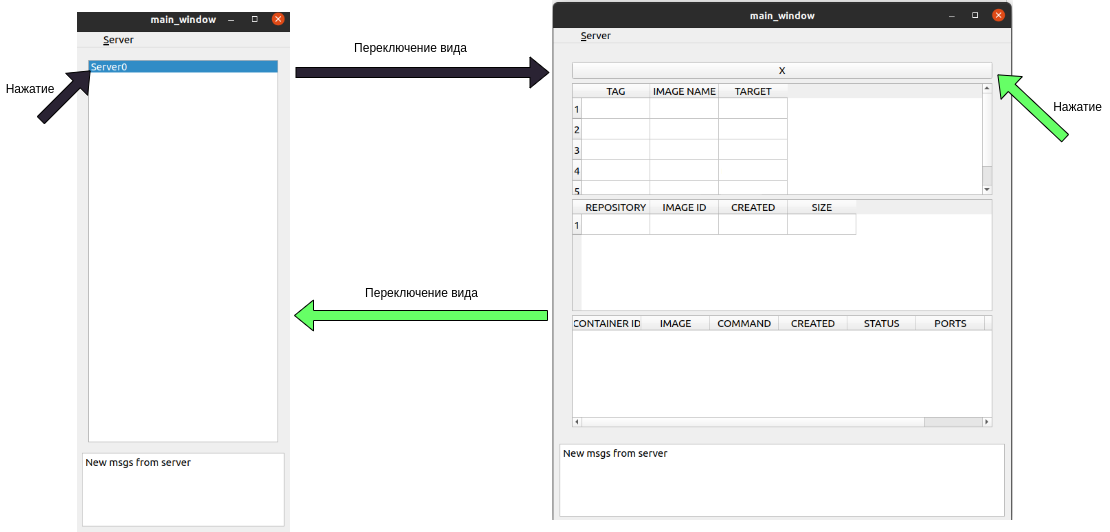
\includegraphics[scale = 0.4]{./figure/gui-stack-wgt}
\caption{Схема переключения вида в ServerWidget}
\label{fig:manip_photo}
\end{center}
\end{figure}
\par После создания необходимых виджетов идет процесс связывания сигналов этих виджетов со слотами класса ServerWidget.
\begin{lstlisting}[language=C++, frame=single, xleftmargin=15pt, caption={Cвязывания сигналов и слотов в ServerWidget},label=DescriptiveLabel]
        connect(srv_name_list_wgt, &QListWidget::itemClicked, this, &ServerWidget::onServerClicked);
        connect(back_button_, &QPushButton::clicked, this, &ServerWidget::onServerBackClicked);
        connect(container_build_table_wgt, &QTableWidget::customContextMenuRequested, this, &ServerWidget::showContextBuild);
        connect(container_name_table_wgt, &QTableWidget::customContextMenuRequested, this, &ServerWidget::showContextName);
        connect(container_run_table_wgt, &QTableWidget::customContextMenuRequested, this, &ServerWidget::showContextRun);
\end{lstlisting}
\par Здесь содержится информация о реагировании каждого из членов графического интерфейса на действия пользователя, например, при 
нажатии на один из серверов в списке srv\_name\_list\_wgt, отправляется сигнал itemClicked, который обрабатывается слотом 
onServerClicked. Внутри метода переключается вид в stack виджете и отрисовываются виджеты ответственные за микросервисы. Интерес 
представляет связь виджетов таблиц. Здесь происходит запрос контекстного меню, которое открывается при нажатии на правую кнопку мыши 
поверх строки таблицы. Для каждой из таблиц создается собственный вид контекстного меню и собственная реакция на предложенные действия.
\begin{figure}[h]
\begin{minipage}[h]{0.49\linewidth}
\center{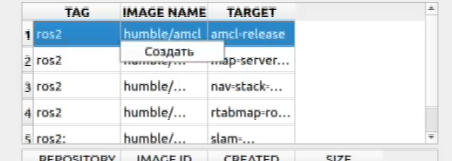
\includegraphics[scale=0.5]{prep_context_menu} \\ a)}
\end{minipage}
\hfill
\begin{minipage}[h]{0.49\linewidth}
\center{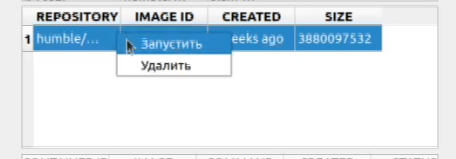
\includegraphics[scale=0.5]{build_context_menu} \\ b)}
\end{minipage}
\hfill
\begin{minipage}[h]{\linewidth}
\center{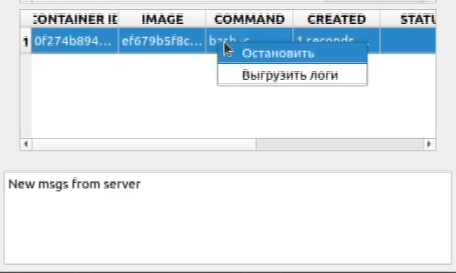
\includegraphics[scale=0.5]{run_context_menu} \\ c)}
\end{minipage}
\caption{Контекстное меню виджетов. a) - образа микросервисы, которые можно собрать, b) - образа микросервисов, которые можно запустить, c) - образа микросервисов, запущенных на сервере}
\label{ris:image1}
\end{figure}
\par Рассмотрим один из методов класса ServerWidget, для того чтобы понять устройство взаимодействия между графическим интерфейсом и 
классом клиента. Например, метод createServer(...)
\begin{lstlisting}[language=C++, frame=single, xleftmargin=15pt, caption={Определение слота createServer},label=DescriptiveLabel]
        ServerCredentalBox* server_cred_ = new ServerCredentalBox();

        if (server_cred_->exec() == QDialog::Accepted)
        {
                wgt_stack->setCurrentIndex(0);
        
                QString server_name("Server");
        
                auto [ip, port] = server_cred_->getIpPort();
                server_name += QString::number(server_counter_);
        
                clients_[server_name] = client_creator_->createRoboClient(ip, port);
        
                if(!clients_[server_name]->createDDSInstance(server_counter_))
                {
                        auto&& erase_it = clients_.find(server_name);
                        clients_.erase(erase_it);
                }
                else
                {
                        QListWidgetItem* server_item_ = new QListWidgetItem(server_name);
                        server_item_->setIcon(QPixmap(":/images/Android.png"));
                
                        srv_name_list_wgt->addItem(server_item_);
                
                        server_counter_++;
                }
        }
\end{lstlisting}
\par Это опредление слота класса ServerWidget, который вызывается в ответ на сигнал от верхнеуровнего меню главного виджета, который 
отправляется при нажатии кнопки создания нового подключения к серверу. На 1 строке идет запуск всплывающего окна диалога, который 
запрашивает у пользователя учетные данные сервера.
\begin{figure}[ht]
\begin{center}
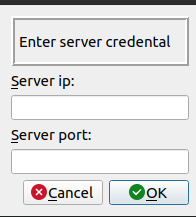
\includegraphics[scale = 0.4]{./figure/cred_dialog}
\caption{Запрос данных сервера}
\label{fig:manip_photo}
\end{center}
\end{figure}
\par Класс ServerCredentalBox реализует функции всплывающего окна и сохраняет учетные данные, как поле класса. Поток выполнения останавливается 
на вызове метода exec(...) объекта server\_cred\_, после ввода данных и нажатие на кнопку "OK", поток выполнения снова возобновляет свою работу.
Вызов метода exec(...) возвращает объект типа enum, который сравнивается с константой Accepted. Это проверка необходима для того, чтобы 
весь дальнейший код внутри if выполнился только в том случае, если пользователь нажал на кнопку "OK". Также, сохранения учетных данных 
в поле класса ServerCredentalBox реализовано на сигнале от нажатия кнопки "OK". На 5 строке идет переключение вида stack виджета, после 
чего идет формирования надписи "Server" с соотвествующим порядковым номером. На строке 9 идет вызов метода, класса диалога, который 
получает учетные данные сервера из полей класса диалога. На 12 строке идет создание класса клиента, с помощью вызова метода класса 
создателя клиентов. Класс клиентов, копируется в отображение расположенное в классе, в нем каждому имени сервера, соответсвует его 
клиент. На строке 14 идет вызова метода класса клиента, которая формирует запрос к серверу с требованием о запуске FastDDS Discovery 
Server, который осуществляет связь между микросервисами и роботом. В случае успеха, сервер добавляется к виджету и отображается на 
экране. В противном случае, такой сервер удаляется.
\chapter{Заключение}
\par В заключении хотелось бы подвести результаты выполненной работы. В исследовании получилось соединить несколько 
технологий для достижения общей цели - запуска алгоритмов одновременного картографирования и локализации. У данного 
решения еще есть много проблем с безопастносью и функционалом, однако, оно уже является продуктом, которым можно 
пользоваться в работе. В дальнейшем можно рассмотреть расширение функционала управления кластером микросервисов,
добавить новые полезные сведения в графических интерфейс пользователя и включить инициализацию FastDDS Discovery Server
через DDS API, однако, в рамках ограниченного времени, решение получилось локаничным и функциональным.
\section{Основные результаты исследования}
\par В качестве цели данной работы, стояла задача создания сетевого сервиса, обеспечивающее управление кластером 
микросервисов, реализующих алгоритм одновременного картографирования и локализации. Ознакомиться с демонстрационным 
видео можно по \href{https://rutube.ru/video/508c42fa971fc0d4260576602548bb51/}{ссылке}. В ходе работы был создан 
прототип сетевого сервиса для управления алгоритмами одновременного картографирования и локализации, реализованный 
с использованием передовых подходов к созданию подобных сервисов. Сервис использует Docker для изоляции и масштабирования 
своих микросервисов.  Для реализации сетевого взаимодействия используется библиотека Boost.Asio, на основе которой 
построен протокол для связи клиентской и серверной части сервиса, что позволилос обеспечить высокую производительность 
и кросплатформенность. Для визуализации и управления разработа графический интерфей пользователя на базе Qt5, 
обеспечивающий интуитивный доступ к функционалу системы. В результате, сервис демонстрирует стабильную работу при 
работе с алгоритмами одновременного картографирования и локализации, подтверждя эффективность выбора технологий и 
архитектуру системы.
\section{Дальнейшее направление исследований}
\par Дальнейшее развитие системы, можно разделить на 3 основных направления:
\begin{itemize}
        \item Расширение функции графического интерфейса. Добавление новых виджетов, позволяющих более полно отображать 
        состояние микросервисов. Например, создания виджета, отображающего граф с микросервисами в вершинах и 
        топиками в качестве ребер. По этому графу будет удобно визуализировать состояние микросервиса и возможные 
        ошибки в его работе.
        \item Расширение протокола связи. Протокол связи построенный на Boost.Asio не позволяет пересылать непрерывные 
        потоки данных, которые бы расширили функционал других подсистем сервиса. Например, потоковая передача данных 
        о состоянии сервиса, позволило бы отображать его состояние в реальном времени. 
        \item Обработка данных. Обработка механизма обработки нуждается в серьезной доработке, т.к. она не позволяет 
        дать пользователю полный контроль над микросервисами.        
\end{itemize}
\par Данный прототип системы позволяет оценить потенциал решений в области Облачной робототехники, однако, для серьезной продуктовой разработки 
роботов он не подходит. Системе нужна дальнейшая поддержка, которая позволила бы реализовать недостающий функционал.
Однако, прототип уже обладает всеми необходимыми функциями, которые требуются для базовой настройки микросервисов,
протестировать работу можно перейдя по \href{https://github.com/sees1/masters}{ссылке} и скачав репозитории с исходным 
кодом данного проекта.
\begin{thebibliography}{9}
        \bibitem{iotBrief}    Gubbi J. и др. Internet of Things (IoT): A vision, architectural elements, and future directions // Future Generation Computer Systems. 2013. Т. 29. № 7. С. 1645–1660.
        \bibitem{iotPrep}  Zhang J., Tao D. Empowering Things with Intelligence: A Survey of the Progress, Challenges, and Opportunities in Artificial Intelligence of Things // 2020.
        \bibitem{cloudRobotics} Hu G., Tay W., Wen Y. Cloud robotics: architecture, challenges and applications // IEEE Network. 2012. Т. 26. № 3. С. 21–28.
        \bibitem{cloudPaper} Miratabzadeh S. A. и др. Cloud robotics: A software architecture: For heterogeneous large-scale autonomous robots // 2016 World Automation Congress (WAC). Rio Grande, PR, USA: IEEE, 2016. С. 1–6.
        \bibitem{dockerCommon}  Muzumdar P. и др. Navigating the Docker Ecosystem: A Comprehensive Taxonomy and Survey // 2024.
        \bibitem{dockerPrep}  Mullinix S. P. и др. On Security Measures for Containerized Applications Imaged with Docker // 2020.
        \bibitem{qt5Book}       Eng L. Z. Qt5 C++ GUI programming cookbook: practical recipes for building cross-platform GUI applications, widgets, and animations with Qt 5. Birmingham, UK: Packt Publishing, 2019. Вып. Second edition. 1 с.
        \bibitem{qt5API}        Qt 5.15 [Электронный ресурс]. URL: \url{https://doc.qt.io/qt-5/}.
        \bibitem{asioBook}      Torjo J., Anggoro W. Boost.Asio C++ network programming: learn effective C++ network programmingwith Boost.Asio and become a proficient C++ network programmer, second edition. Birmingham: Packt Publishing, 2015. Вып. 2nd ed. 1 с.
        \bibitem{asioPap}       Kadusic E. и др. The transitional phase of Boost.Asio and POCO C++ networking libraries towards IPv6 and IoT networking security // 2022 IEEE International Conference on Smart Internet of Things (SmartIoT). Suzhou, China: IEEE, 2022. С. 80–85.       
        \bibitem{microServiceBook}  Newman S. Building microservices: designing fine-grained systems. Beijing Sebastopol, CA: O’Reilly Media, 2015. Вып. First Edition. 259 с.
        \bibitem{microServiceBook1} Nadareishvili I. Microservice architecture: aligning principles, practices, and culture. Sebastopol, CA: O’Reilly Media, Inc, 2016. Вып. First edition. 128 с.
        \bibitem{soaBook}     Erl T. Service-oriented architecture: concepts, technology, and design. Upper Saddle River, NJ Munich: Prentice Hall PTR, 2009. Вып. 9. print. 760 с.
        \bibitem{soaBook1}     Lawler J. P., Howell-Barber H. Service-oriented architecture: SOA strategy, methodology, and technology. Boca Raton: Auerbach, 2019.
        \bibitem{serverlessBook}  Gilbert J. Software Architecture Patterns for Serverless Systems: Architecting for innovation with event-driven microservices and micro frontends. Birmingham: Packt Publishing Limited, 2024. Вып. 1. 1 с.
        \bibitem{serverlessBook1} Sbarski P. Serverless architectures on AWS. Shelter Island: Manning, 2017. 354 с.
        \bibitem{serverlessArt1}  Saji J., Kumar A. A Review Paper on Serverless Architecture of Web Applications // SSRN Journal. 2024.
        \bibitem{edaBook}     Percival H. J. W., Gregory B. Architecture patterns with Python: enabling test-driven development, domain-driven design, and event-driven microservices. Beijing Boston Farnham Sebastopol Tokyo: O’Reilly, 2020. Вып. First edition. 1 с.
        \bibitem{protocolBook}  Олифер В. Компьютерные сети. Принципы, технологии, протоколы. Санкт-Петербург: Питер, 2021. Вып. Юбилейное издание. 1008 с.
        \bibitem{protocolArt1}  Gamal A. E., Kim Y.-H. Lecture Notes on Network Information Theory // 2010.
        \bibitem{guiBrief}      Martinez W. L. Graphical user interfaces // WIREs Computational Stats. 2011. Т. 3. № 2. С. 119–133.
        \bibitem{guiArt1}      Martinez W. L. Graphical user interfaces // WIREs Computational Stats. 2011. Т. 3. № 2. С. 119–133.
        \bibitem{compLangArt}  Ernest A., Mensah E., Gilbert A. Qualitative Assessment of Compiled, Interpreted and Hybrid Programming Languages // CAE. 2017. Т. 7. № 7. С. 8–13.
        \bibitem{compLangBook}  Aho A. V., Sethi R., Ullman J. D. Compilers, principles, techniques, and tools. Reading, Mass: Addison-Wesley Pub. Co, 1986. 796 с.
        \bibitem{cppBook}     Stroustrup B. The C++ programming language: C++ 11. Upper Saddle River, NJ: Addison-Wesley, 2015. Вып. 4. ed., 4. print. 1347 с.
        \bibitem{cppArt1}  Rassokhin D. The C++ programming language in cheminformatics and computational chemistry // J Cheminform. 2020. Т. 12. № 1. С. 10.
        \bibitem{rosMain}     Macenski S. и др. Robot Operating System 2: Design, architecture, and uses in the wild // Sci. Robot. 2022. Т. 7. № 66. С. eabm6074.
        \bibitem{rosPrep}     Macenski S. и др. Impact of ROS 2 Node Composition in Robotic Systems // 2023.
        \bibitem{ddsMain}     Corsaro A., C. D. The Data Distribution Service – The Communication Middleware Fabric for Scalable and Extensible Systems-of-Systems // System of Systems / под ред. A. V. Gheorghe. : InTech, 2012.
        \bibitem{ddsBook}     Mahmood Z. Connected Environments for the Internet of Things: Challenges and Solutions. Cham: Springer, 2018. 269–285 с.
        \bibitem{cmakeBook}   Martin K., Hoffman B. Mastering CMake: Version 3.1. Clifton Park, NY.: Kitware Inc, 2015. 700 с.
        \bibitem{cmakeArt}    Crandall Z. и др. CMakePPLang: An object-oriented extension toCMake // JOSS. 2023. Т. 8. № 89. С. 5 с.
        \bibitem{buildSystBook}  Smith P. Software build systems: principles and experience. Upper Saddle River, N.J: Addison Wesley, 2011. 583 с.
        \bibitem{buildSystArt} Mokhov A., Mitchell N., Peyton Jones S. Build systems à la carte // Proc. ACM Program. Lang. 2018. Т. 2. № ICFP. С. 1–29.
        \bibitem{cliBook}  Shotts W. E. The Linux command line: a complete introduction. San Francisco: No Starch Press, 2012. 504 с.
        \bibitem{cliPrep}  Voronkov A., Martucci L. A., Lindskog S. System Administrators Prefer Command Line Interfaces, Don’t They? An Exploratory Study of Firewall Interfaces // 2019.
        \bibitem{pythonBook} Zelle J. M. Python programming: an introduction to computer science. Portland: Franklin, Beedle \& Associates Inc, 2024. Вып. Fourth edition. 574 с.
        \bibitem{pythonBook1}  Urban M., Murach J. Murachs Python programming: beginner to pro. Fresno, CA: Mike Murach \& Associates, Inc., 2021. Вып. 2nd edition.
        \bibitem{sdpOverview} Simple Participant Discovery [Электронный ресурс]. URL: \url{https://community.rti.com/static/documentation/connext-dds/current/doc/manuals/connext_dds_professional/users_manual/users_manual/Simple_Participant_Discovery.htm}.
        \bibitem{unixBook}  Negus C. Linux Bible, 10th Edition. Erscheinungsort nicht ermittelbar: Wiley, 2020. Вып. 10th edition. 1556 с.
        \bibitem{unixBook1}  Stallman R., Lessig L. Free software, free society: selected essays of Richard Stallman. Boston, MA: Free Software Foundation, 2010. Вып. 2nd ed.
        \bibitem{slamMain}  Scaradozzi D., Zingaretti S., Ferrari A. Simultaneous localization and mapping (SLAM) robotics techniques: a possible application in surgery // Shanghai Chest. 2018. Т. 2. С. 5–5.
        \bibitem{slamArt0}  Kudriashov A. SLAM Techniques Application for Mobile Robot in Rough Terrain. Cham: Springer International Publishing AG, 2020. 131 с.
        \bibitem{amrBook}   Kala R. Autonomous mobile robots: planning, navigation and simulation. London: Academic Press, 2024. 1064 с.
        \bibitem{bayesBook} Särkkä S., Svensson L. Bayesian Filtering and Smoothing. : Cambridge University Press, 2023. Вып. 2.
        \bibitem{bayesArt}  Kutschireiter A. и др. Nonlinear Bayesian filtering and learning: a neuronal dynamics for perception // Sci Rep. 2017. Т. 7. № 1. С. 8722.
        \bibitem{slamArt1}  Placed J. A. и др. A Survey on Active Simultaneous Localization and Mapping: State of the Art and New Frontiers // IEEE Transactions on Robotics (T-RO). 2022. С. 1–20.
        \bibitem{slamArt2}  Boal J., Sánchez-Miralles Á., Arranz Á. Topological simultaneous localization and mapping: a survey // Robotica. 2014. Т. 32. № 5. С. 803–821.
        \bibitem{slamArt3}  Kitanov A., Indelman V. Topological belief space planning for active SLAM with pairwise Gaussian potentials and performance guarantees // The International Journal of Robotics Research. 2024. Т. 43. № 1. С. 69–97.
        \bibitem{slamArt4}  Chen K. и др. Semantic Visual Simultaneous Localization and Mapping: A Survey // 2022.
        \bibitem{slamPap1}  Bowman S. L. и др. Probabilistic data association for semantic SLAM // 2017 IEEE International Conference on Robotics and Automation (ICRA). Singapore, Singapore: IEEE, 2017. С. 1722–1729.
        \bibitem{amclArt}   Das S. Robot localization in a mapped environment using Adaptive Monte Carlo algorithm // 2025.
        \bibitem{amclArt1}  Zuo C. и др. An Improved Adaptive Monte Carlo Localization Algorithm Integrated with a Virtual Motion Model // Sensors. 2025. Т. 25. № 8. С. 2471.
        \bibitem{gmclArt}   Alshikh K., Mhd A., Lyad H. gmcl As a Proposed Replacement to amcl in ROS for Mobile Robots Localization in Known-Based 2D Environments. // 2021.
        \bibitem{hectorPap} Kohlbrecher S. и др. A flexible and scalable SLAM system with full 3D motion estimation // 2011 IEEE International Symposium on Safety, Security, and Rescue Robotics. Kyoto, Japan: IEEE, 2011. С. 155–160.
        \bibitem{rtabmapArt}  Labbe M., Michaud F. RTAB-Map as an open-source lidar and visual simultaneous localization and mapping library for large-scale and long-term online operation // Journal of Field Robotics. 2019. Т. 36. № 2. С. 416–446.
        \bibitem{cartographerArt} Hess W. и др. Real-time loop closure in 2D LIDAR SLAM // 2016 IEEE International Conference on Robotics and Automation (ICRA). Stockholm, Sweden: IEEE, 2016. С. 1271–1278.
        \bibitem{osiArt}  Zimmermann H. OSI Reference Model--The ISO Model of Architecture for Open Systems Interconnection // IEEE Trans. Commun. 1980. Т. 28. № 4. С. 425–432.
        \bibitem{osiArt1} Day J. D., Zimmermann H. The OSI reference model // Proc. IEEE. 1983. Т. 71. № 12. С. 1334–1340.
        \bibitem{pocoDoc} POCO C++ Libraries - Reference Library [Электронный ресурс]. URL: \url{https://docs.pocoproject.org/current/}.
        \bibitem{aceBook} Schmidt D. C., Huston S. D. C++ network programming. Boston: Addison-Wesley, 2002.
        \bibitem{ipcBook} Silberschatz A., Galvin P. B., Gagne G. Operating system concepts. Hoboken, NJ: Wiley, 2018. Вып. Tenth edition.
        \bibitem{patternBook} Design patterns: elements of reusable object-oriented software / под ред. E. Gamma. Boston, Mass. Munich: Addison-Wesley, 2011. Вып. 39. printing. 395 с.
        \bibitem{patternArt1} Schmidt D. C. Using design patterns to develop reusable object-oriented communication software // Commun. ACM. 1995. Т. 38. № 10. С. 65–74.
        \bibitem{concurrBook} Williams A. C++ concurrency in action. Shelter Island, NY: Manning Publications Co, 2019. Вып. Second edition. 568 с.
        \bibitem{concurrArt1}  Herlihy M. The art of multiprocessor programming // Proceedings of the twenty-fifth annual ACM symposium on Principles of distributed computing. Denver Colorado USA: ACM, 2006. С. 1–2.
        \bibitem{umlArt} UML distilled: a brief guide to the standard object modeling language / под ред. M. Fowler. Boston, Mass.: Addison-Wesley, 2010. Вып. 3. ed, 16. printing. 175 с.
        \bibitem{dockerApi} Docker Engine API v1.48 reference [Электронный ресурс]. URL: \url{https://docs.docker.com/reference/api/engine/version/v1.48/}.
        \bibitem{sharedMemArt} Diener M. и др. Communication in Shared Memory: Concepts, Definitions, and Efficient Detection // 2016 24th Euromicro International Conference on Parallel, Distributed, and Network-Based Processing (PDP). Heraklion, Crete, Greece: IEEE, 2016. С. 151–158.
        \bibitem{reflectArt} Maes P. Concepts and experiments in computational reflection // SIGPLAN Not. 1987. Т. 22. № 12. С. 147–155.

\end{thebibliography} 

\end{document}
